\documentclass[11pt]{article}

% ---------- Packages ----------
\usepackage[margin=1in]{geometry}
\usepackage{amsmath,amsthm,graphicx,enumitem,amssymb}
\usepackage{mathtools}
\usepackage{physics}        % derivatives, bras/kets, etc.
\usepackage{siunitx}        % units
\usepackage{graphicx}       % figures
\usepackage{subcaption}     % subfigures
\usepackage{float}          % figure placement
\usepackage{booktabs}       % nice tables
\usepackage{enumitem}       % better lists
\usepackage{fancyhdr}       % header/footer
\usepackage{titlesec}       % section formatting
\usepackage{hyperref}       % links
\usepackage{tcolorbox}      % boxes for answers
\usepackage{listings}       % code (MATLAB, Python, etc.)
\usepackage{xcolor}
\usepackage{bbm}        % blackboard bold italic
\usepackage{xcolor}

% Define colors
\definecolor{codegreen}{rgb}{0,0.6,0}
\definecolor{codepurple}{rgb}{0.58,0,0.82}
\definecolor{backcolour}{rgb}{0.95,0.95,0.92}

% ---------- Hyperref Setup ----------
\hypersetup{
    colorlinks=true,
    linkcolor=blue,
    urlcolor=blue,
    citecolor=blue
}

% ---------- Header/Footer ----------
\pagestyle{fancy}
\fancyhf{}
\lhead{\textbf{\course}}
\rhead{\textbf{\assignment}}
\cfoot{\thepage}

% ---------- Custom Commands ----------
\newcommand{\course}{ASEN 6044}
\newcommand{\assignment}{Homework \#3}
\newcommand{\studentname}{Bijan Jourabchi}

\newcommand{\R}{\mathbb{R}}
\newcommand{\E}{\mathbb{E}}
\newcommand{\Var}{\mathrm{Var}}
\newcommand{\Cov}{\mathrm{Cov}}

% Boxed answer environment
\newtcolorbox{answerbox}{
    colback=gray!5,
    colframe=gray!50,
    title=Answer,
    fonttitle=\bfseries
}

% Problem section format
\titleformat{\section}{\large\bfseries}{Problem \thesection:}{0.5em}{}

% ---------- Code Style ----------
\lstset{
    basicstyle=\ttfamily\small,
    keywordstyle=\color{blue},
    commentstyle=\color{green!50!black},
    stringstyle=\color{orange},
    breaklines=true,
    frame=single
    extendedchars=true,
    literate={π}{{$\pi$}}1 {γ}{{$\gamma$}}1
}
\lstdefinestyle{matlab}{
  language=Matlab,
  basicstyle=\ttfamily\small,
  numbers=left,
  numberstyle=\tiny,
  stepnumber=1,
  numbersep=8pt,
  showstringspaces=false,
  breaklines=true,
  breakatwhitespace=true,
  tabsize=4,
  frame=single,
  captionpos=b
}

% ---------- Document ----------
\begin{document}

% ---------- Title Block ----------
\begin{center}
    {\LARGE \textbf{\course}} \\[6pt]
    {\Large \assignment} \\[10pt]
    \studentname \\
\end{center}

\vspace{1em}
\hrule
\vspace{1em}

% Define Julia language manually
\lstdefinelanguage{Julia}{
  keywords={abstract, break, case, catch, const, continue, do, else, elseif,
      end, export, false, for, function, global, if, import, in, let, local,
      macro, module, otherwise, quote, return, struct, switch, true, try,
      type, typealias, using, while, mutable},
  keywordstyle=\color{blue}\bfseries,
  comment=[l]{\#},
  morecomment=[n]{\#=}{=\#},
  commentstyle=\color{codegreen}\ttfamily,
  stringstyle=\color{codepurple}\ttfamily,
  morestring=[b]',
  morestring=[b]"
}

% General Listing Settings
\lstset{
    language=Julia,
    backgroundcolor=\color{backcolour},   
    basicstyle=\ttfamily\small,
    breaklines=true,                 
    numbers=left,                    
    numbersep=5pt,                  
    frame=single
}

% =====================================================
\section{}

\begin{enumerate}[label = \alph*)]
    \item 
        Given the following prior information on independent state $x$, measurment bias $z$, and measurment likelihood $P(y \mid x,z)$
        \begin{align*}
            p(x) &= \mathcal{U}[1,11] \quad \quad p(z) = \mathcal{G}(a,b) = \frac{1}{b^a \Gamma(a)}z^{a-1}e^{-z/b} \\
            P(y \mid x,z) &=  \mathcal{U}[x,(x+z)^2]
        \end{align*}
        with $a = b = 2$. We can derive the joint distribution as $P(x,z) = P(x)P(z)$ since x and z are independent. To determine the joint posterior PDF, $P(x,z \mid y_1, y_2,\ldots, y_n)$ for a static state (not changing),  we can use bayes rule.
        \begin{align*}
            P(x,z \mid y_1, y_2,\ldots, y_n) = \frac{P(x,z \mid y_1, y_2,\ldots, y_{n-1})P(y_n \mid x,z)}{P(y_1, y_2,\ldots, y_n)}
        \end{align*}

        Thus, for the first measurment $y_1 = 91.56$ we have 
        \begin{align*}
            P(x,z \mid y_1) = \frac{P(x,z)P(y_1 \mid x,z)}{P(y_1)}
        \end{align*}
        We can derive similar expressions for subsequent measurments $y_2$ and $y_3$,
        \begin{align*}
            P(x,z \mid y_1, y_2) &= \frac{P(x,z \mid y_1 )P(y_2 \mid x,z)}{P(y_1,y_2)} \\
            P(x,z \mid y_1, y_2, y_3) &= \frac{P(x,z\mid y_1, y_2)P(y_3 \mid x,z)}{P(y_1,y_2,y_3)} \\
        \end{align*}
        Coding this up using the given intervals for $x$ and $z$, we can plot the joint posteriors seen in figures (\ref{fig:y1}),(\ref{fig:y2}), and (\ref{fig:y3}).
        We see that after each subsequent measurment, the probability density changes slightly each time. This is due to each new measurment encoding more information on what the state could be.
        \begin{figure}[H]
            \centering
                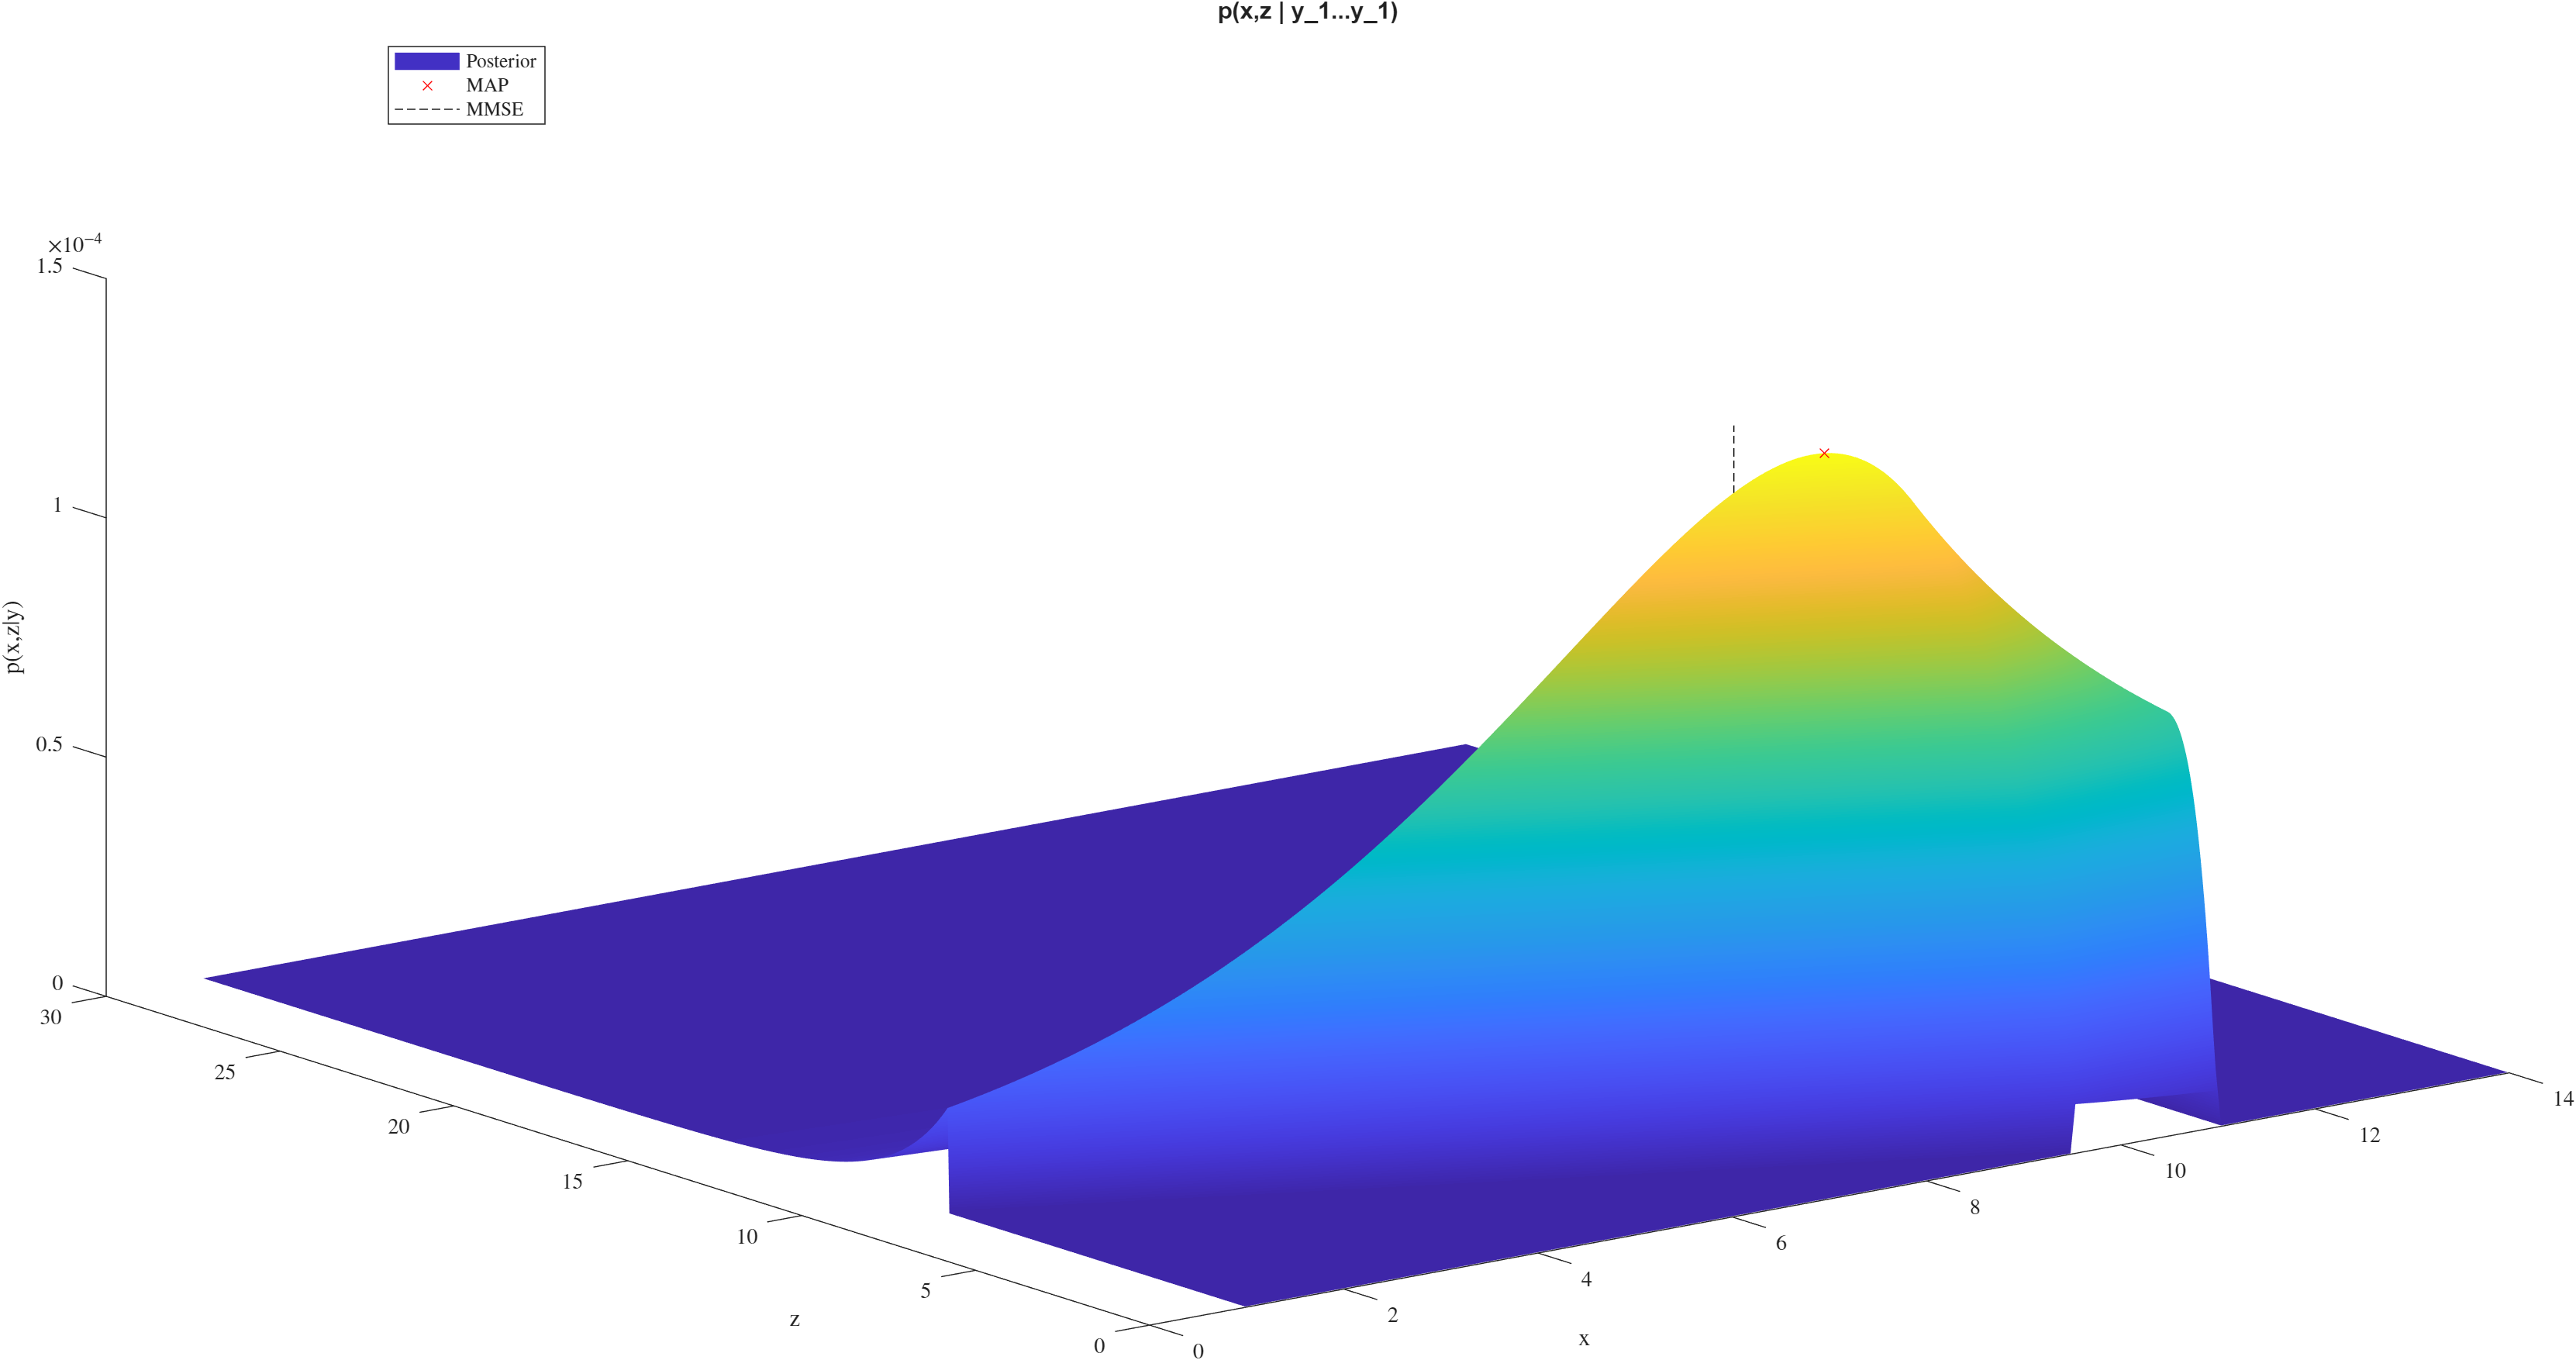
\includegraphics[width=\textwidth, height=\textheight, keepaspectratio]{Measurment_1.png}
            \caption{Joint Posterior $p(x,z \mid y_1)$}
            \label{fig:y1}
        \end{figure}

        \begin{figure}[H]
            \centering
                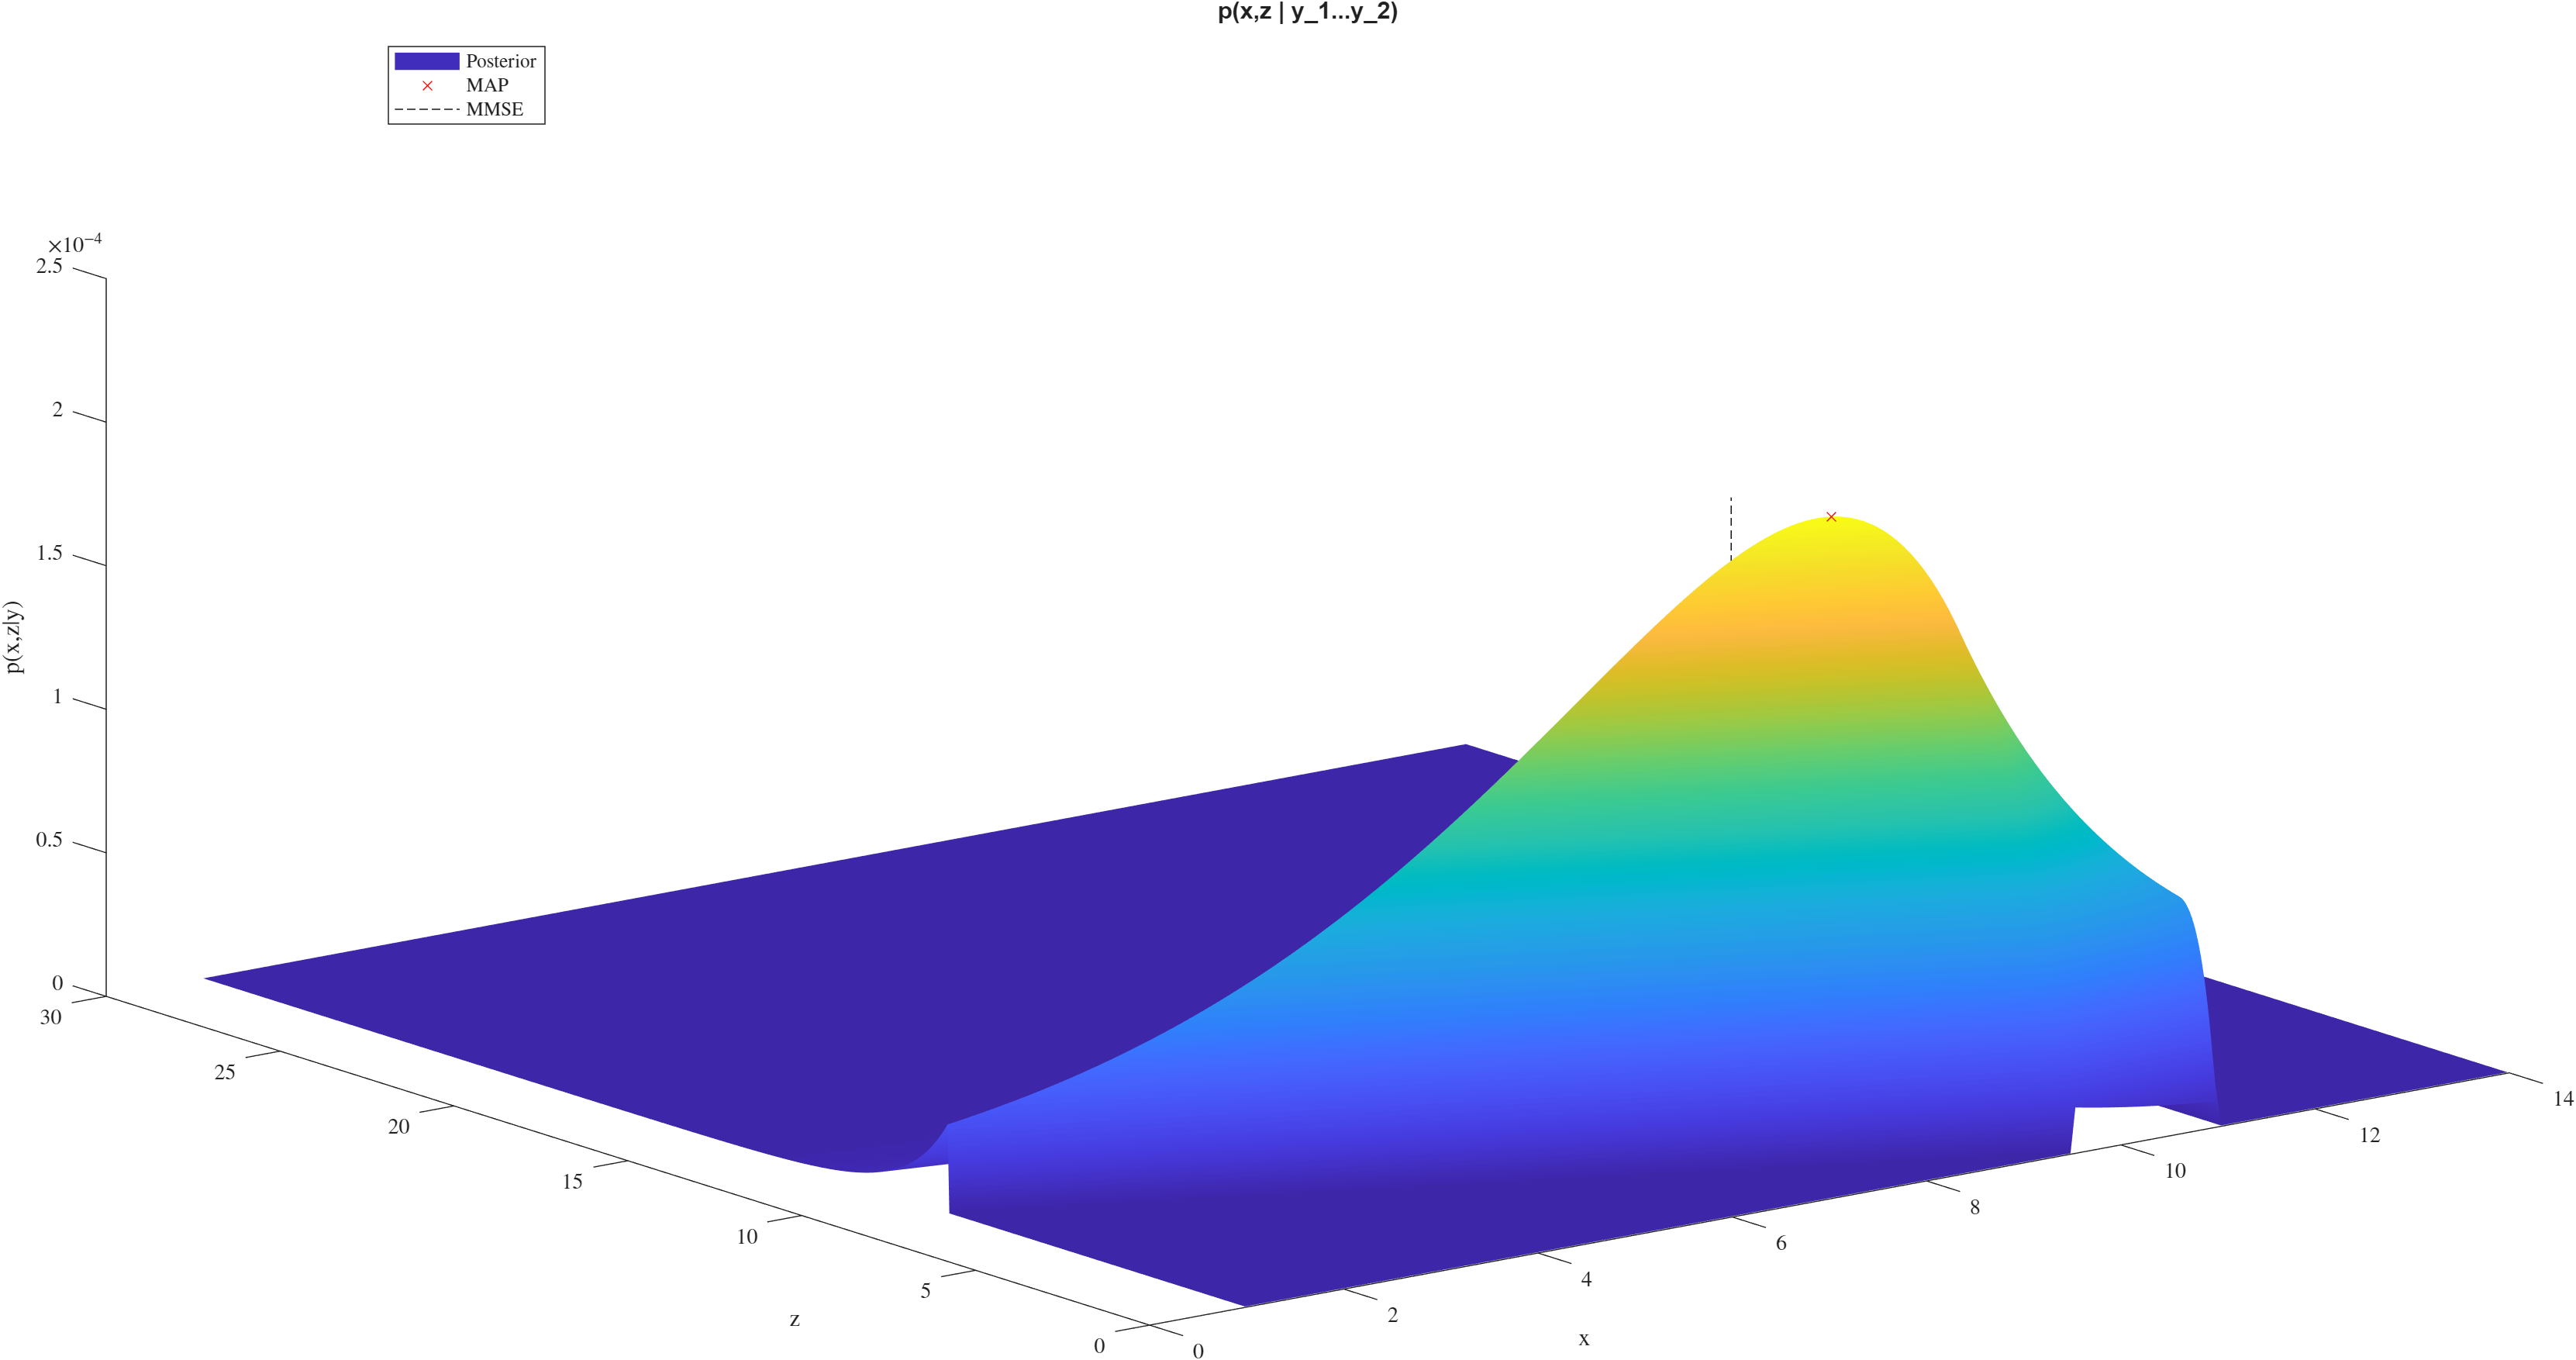
\includegraphics[width=\textwidth, height=\textheight, keepaspectratio]{Measurment_2.png}
            \caption{Joint Posterior $p(x,z \mid y_1,y_2)$}
            \label{fig:y2}
        \end{figure}

        \begin{figure}[H]
            \centering
                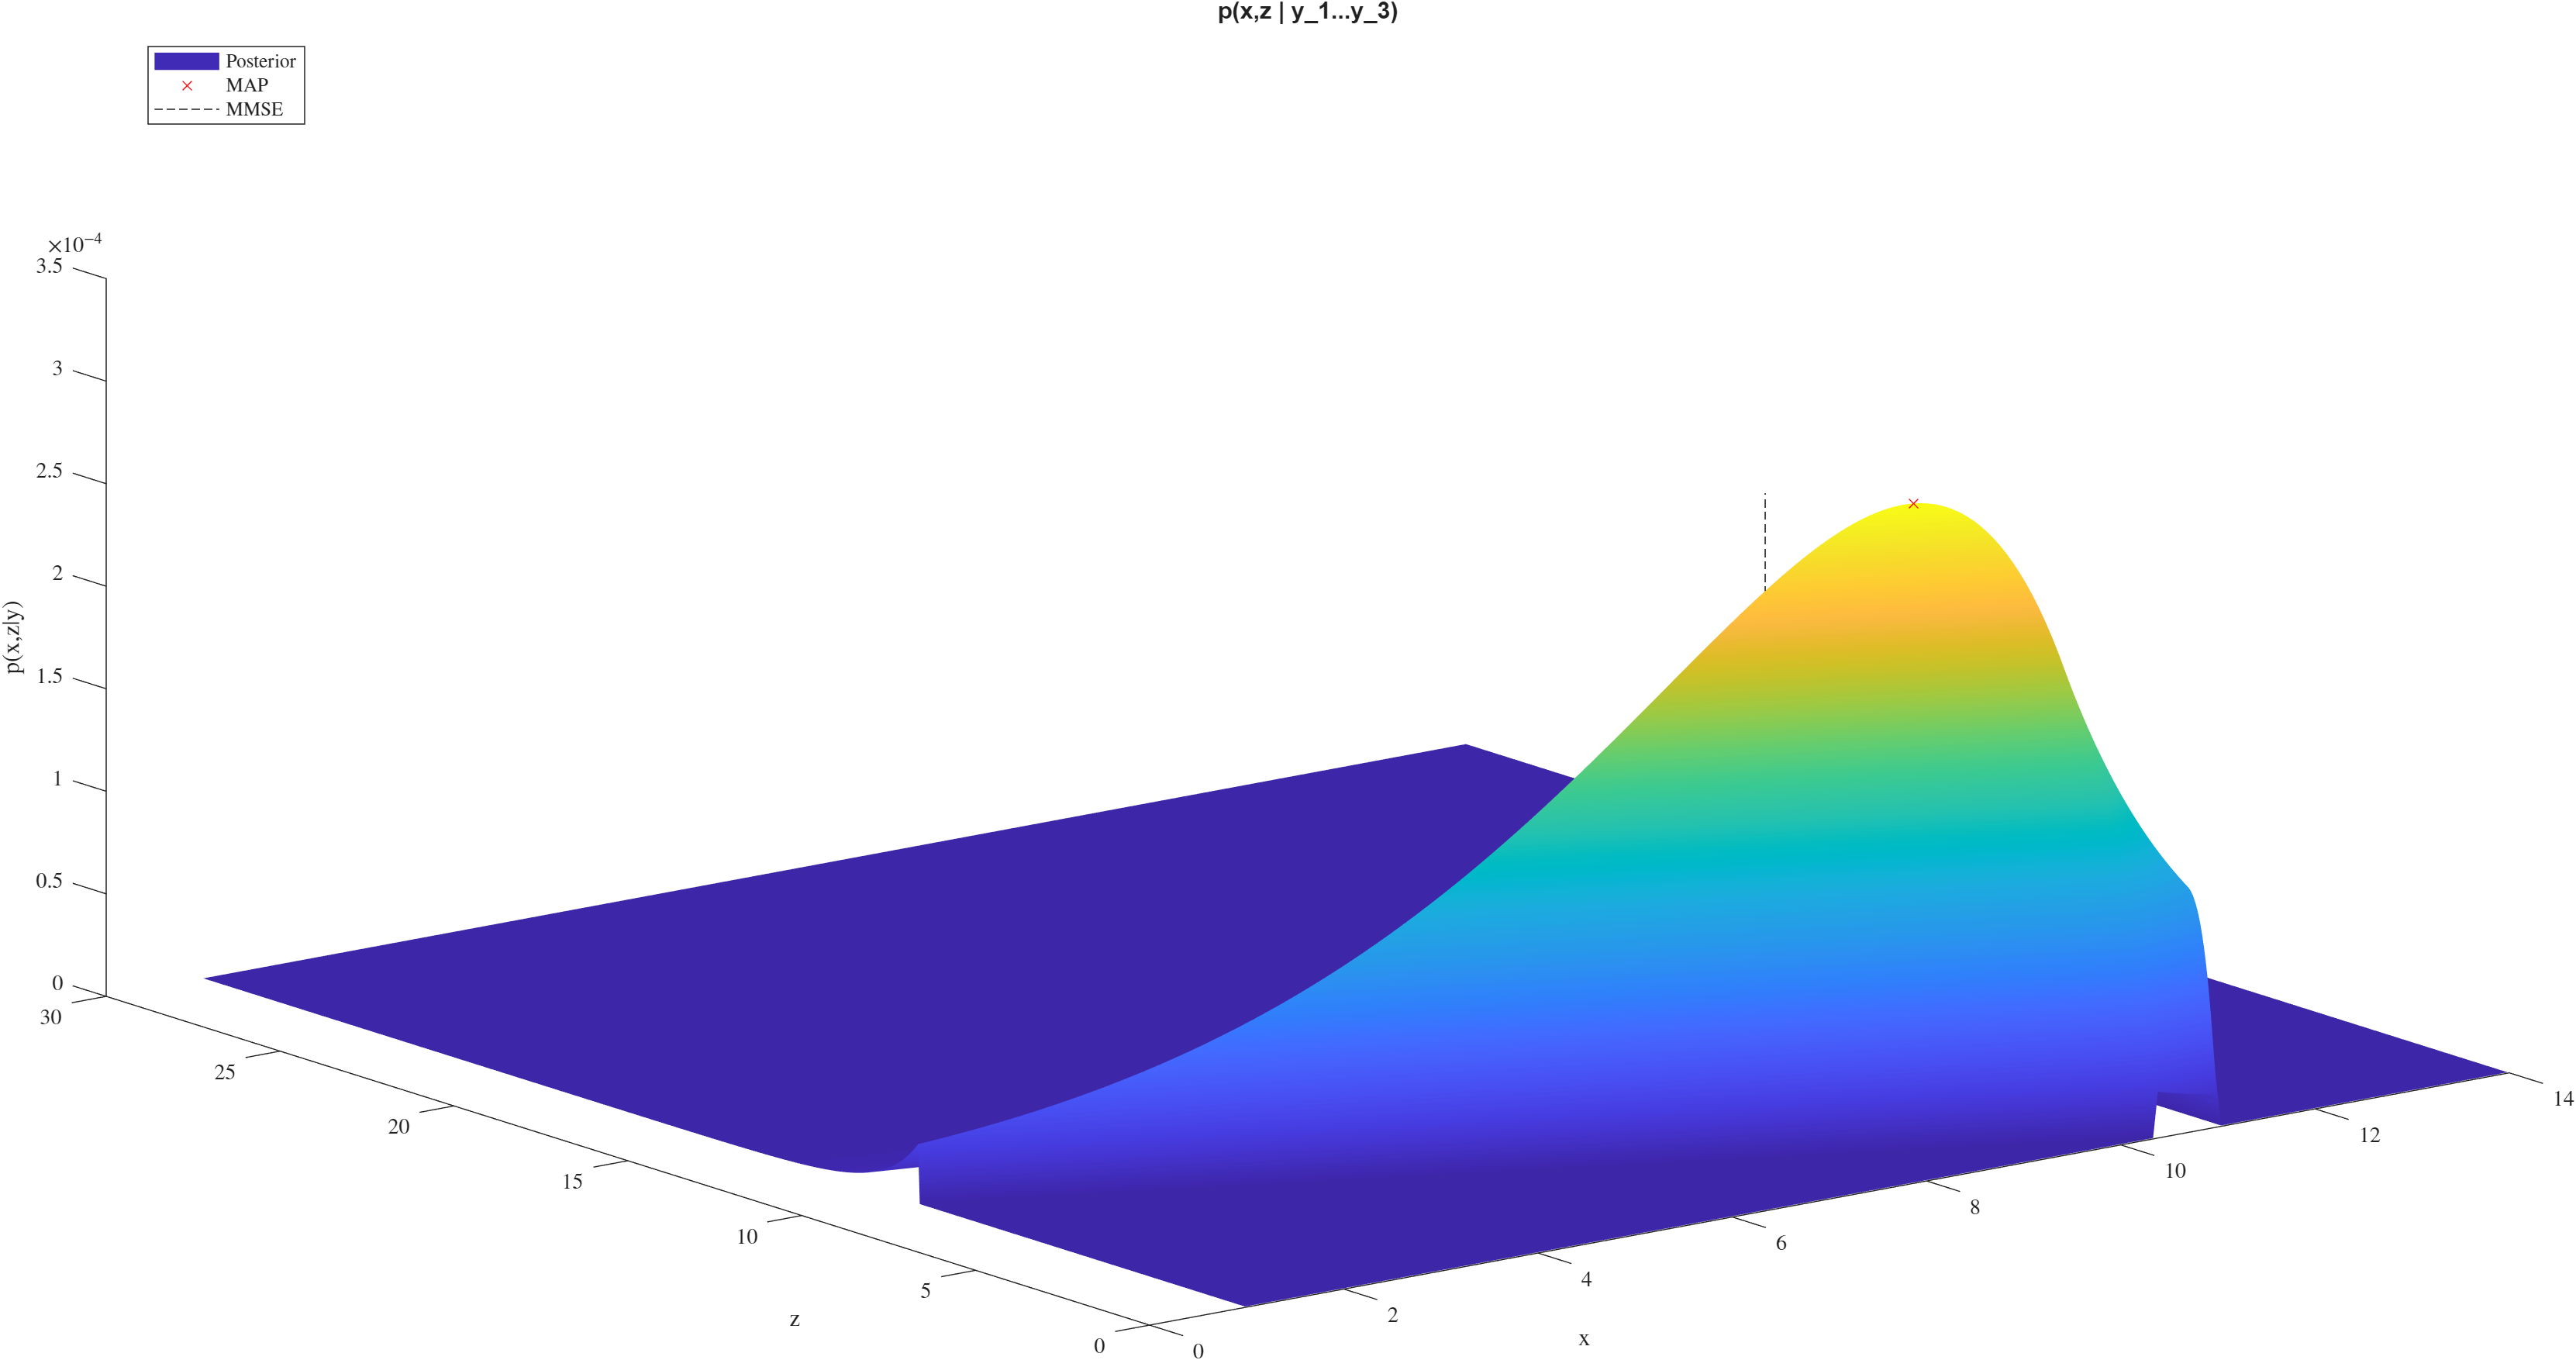
\includegraphics[width=\textwidth, height=\textheight, keepaspectratio]{Measurment_3.png}
            \caption{Joint Posterior $p(x,z \mid y_1, y_2,y_3)$}
            \label{fig:y3}
        \end{figure}

        \item 
        Using the result from part a, we can easily determine the MMSE and MAP estimates of each joint posterior distribution.
        Table~\ref{tab:q1b_estimates} summarizes these estimates for the three posterior distributions.

        \begin{table}[H]
            \centering
            \caption{MMSE and MAP estimates for the joint posterior distributions}
            \label{tab:q1b_estimates}
            \begin{tabular}{ccccc}
                \toprule
                Posterior & MMSE $\hat{z}$ & MMSE $\hat{x}$ & MAP $\hat{z}$ & MAP $\hat{x}$ \\
                \midrule
                $p(x,z \mid y_1)$ & 4.5064 & 7.6296 & 1.95 & 7.65 \\
                $p(x,z \mid y_1,y_2)$ & 4.0683 & 7.4447 & 1.9 & 7.7 \\
                $p(x,z \mid y_1,y_2,y_3)$ & 4.0755 & 7.7973 & 1.9 & 8.55 \\
                \bottomrule
            \end{tabular}
        \end{table}
        
        The value of the marginal data likelihoods $P(y_1),P(y_1,y_2),P(y_1,y_2,y_3)$ are the same as the normalization constants used when normalizing the joint posteriors.
        These values are $P(y_1) = 3.634 \times 10^{-3}$, $P(y_1,y_2) = 7.8\times 10^{-3}$, and, $P(y_1,y_2, y_3) = 5.01\times 10^{-3}$.

        \item
        Before performing Monte Carlo IS, we must derive an expression for the weights. The prior of $P(x,z \mid y_1,y_2,y_3)$ is just the joint posterior after recieving the second measurment, or $q(x,z; y_1,y_2,y_3) = P(x,z \mid y_1,y_2)$.
        The weights for IS are given as the ratio of the distribution we are trying to approximate, $P(x,z \mid y_1,y_2,y_3)$ to the proposal distribution. In this case we can simplify the expression for the importance weights.
        \begin{align*}
            w(X^i_s) = \frac{P(x_i,z_i \mid y_1,y_2,y_3)}{P(x_i,z_i \mid y_1,y_2)} \propto \frac{P(x_i,z_i\mid y_1, y_2)P(y_3 \mid x_i,z_i)}{P(x_i,z_i \mid y_1,y_2)} = P(y_3 \mid x_i,z_i)
        \end{align*}

        Thus, the weight of a sampled point is proportional to the measurment likelihood of $y_3$. Thus, the particle weight for a sampled point $x_s$ is
        \begin{align*}
            \tilde{w}(X^i_s) = \frac{w(X^i_s)}{\sum_{i=1}^{N_s} w(X^i_s)}
        \end{align*}
        Performing IS with 500 samples, we get the result seen in figure (\ref{fig:IS}). The MMSE estimate from the IS particles is the weighted sum of the particles. Computing this, we get a MMSE estimate of $\hat{x}_{MMSE,IS} = 4.21$ and $\hat{z}_{MMSE,IS} = 7.63$.
        Comparing this result from the MMSE value from Table \ref{tab:q1b_estimates}, we see that the two are very similar. While the MMSE estimate from IS is slightly different than that of the exact grid based solution, importance sampling allows us to only sample the important areas of the state space. The loss of accuracy is traded off for the lighter computational load.
        \begin{figure}[H]
            \centering
                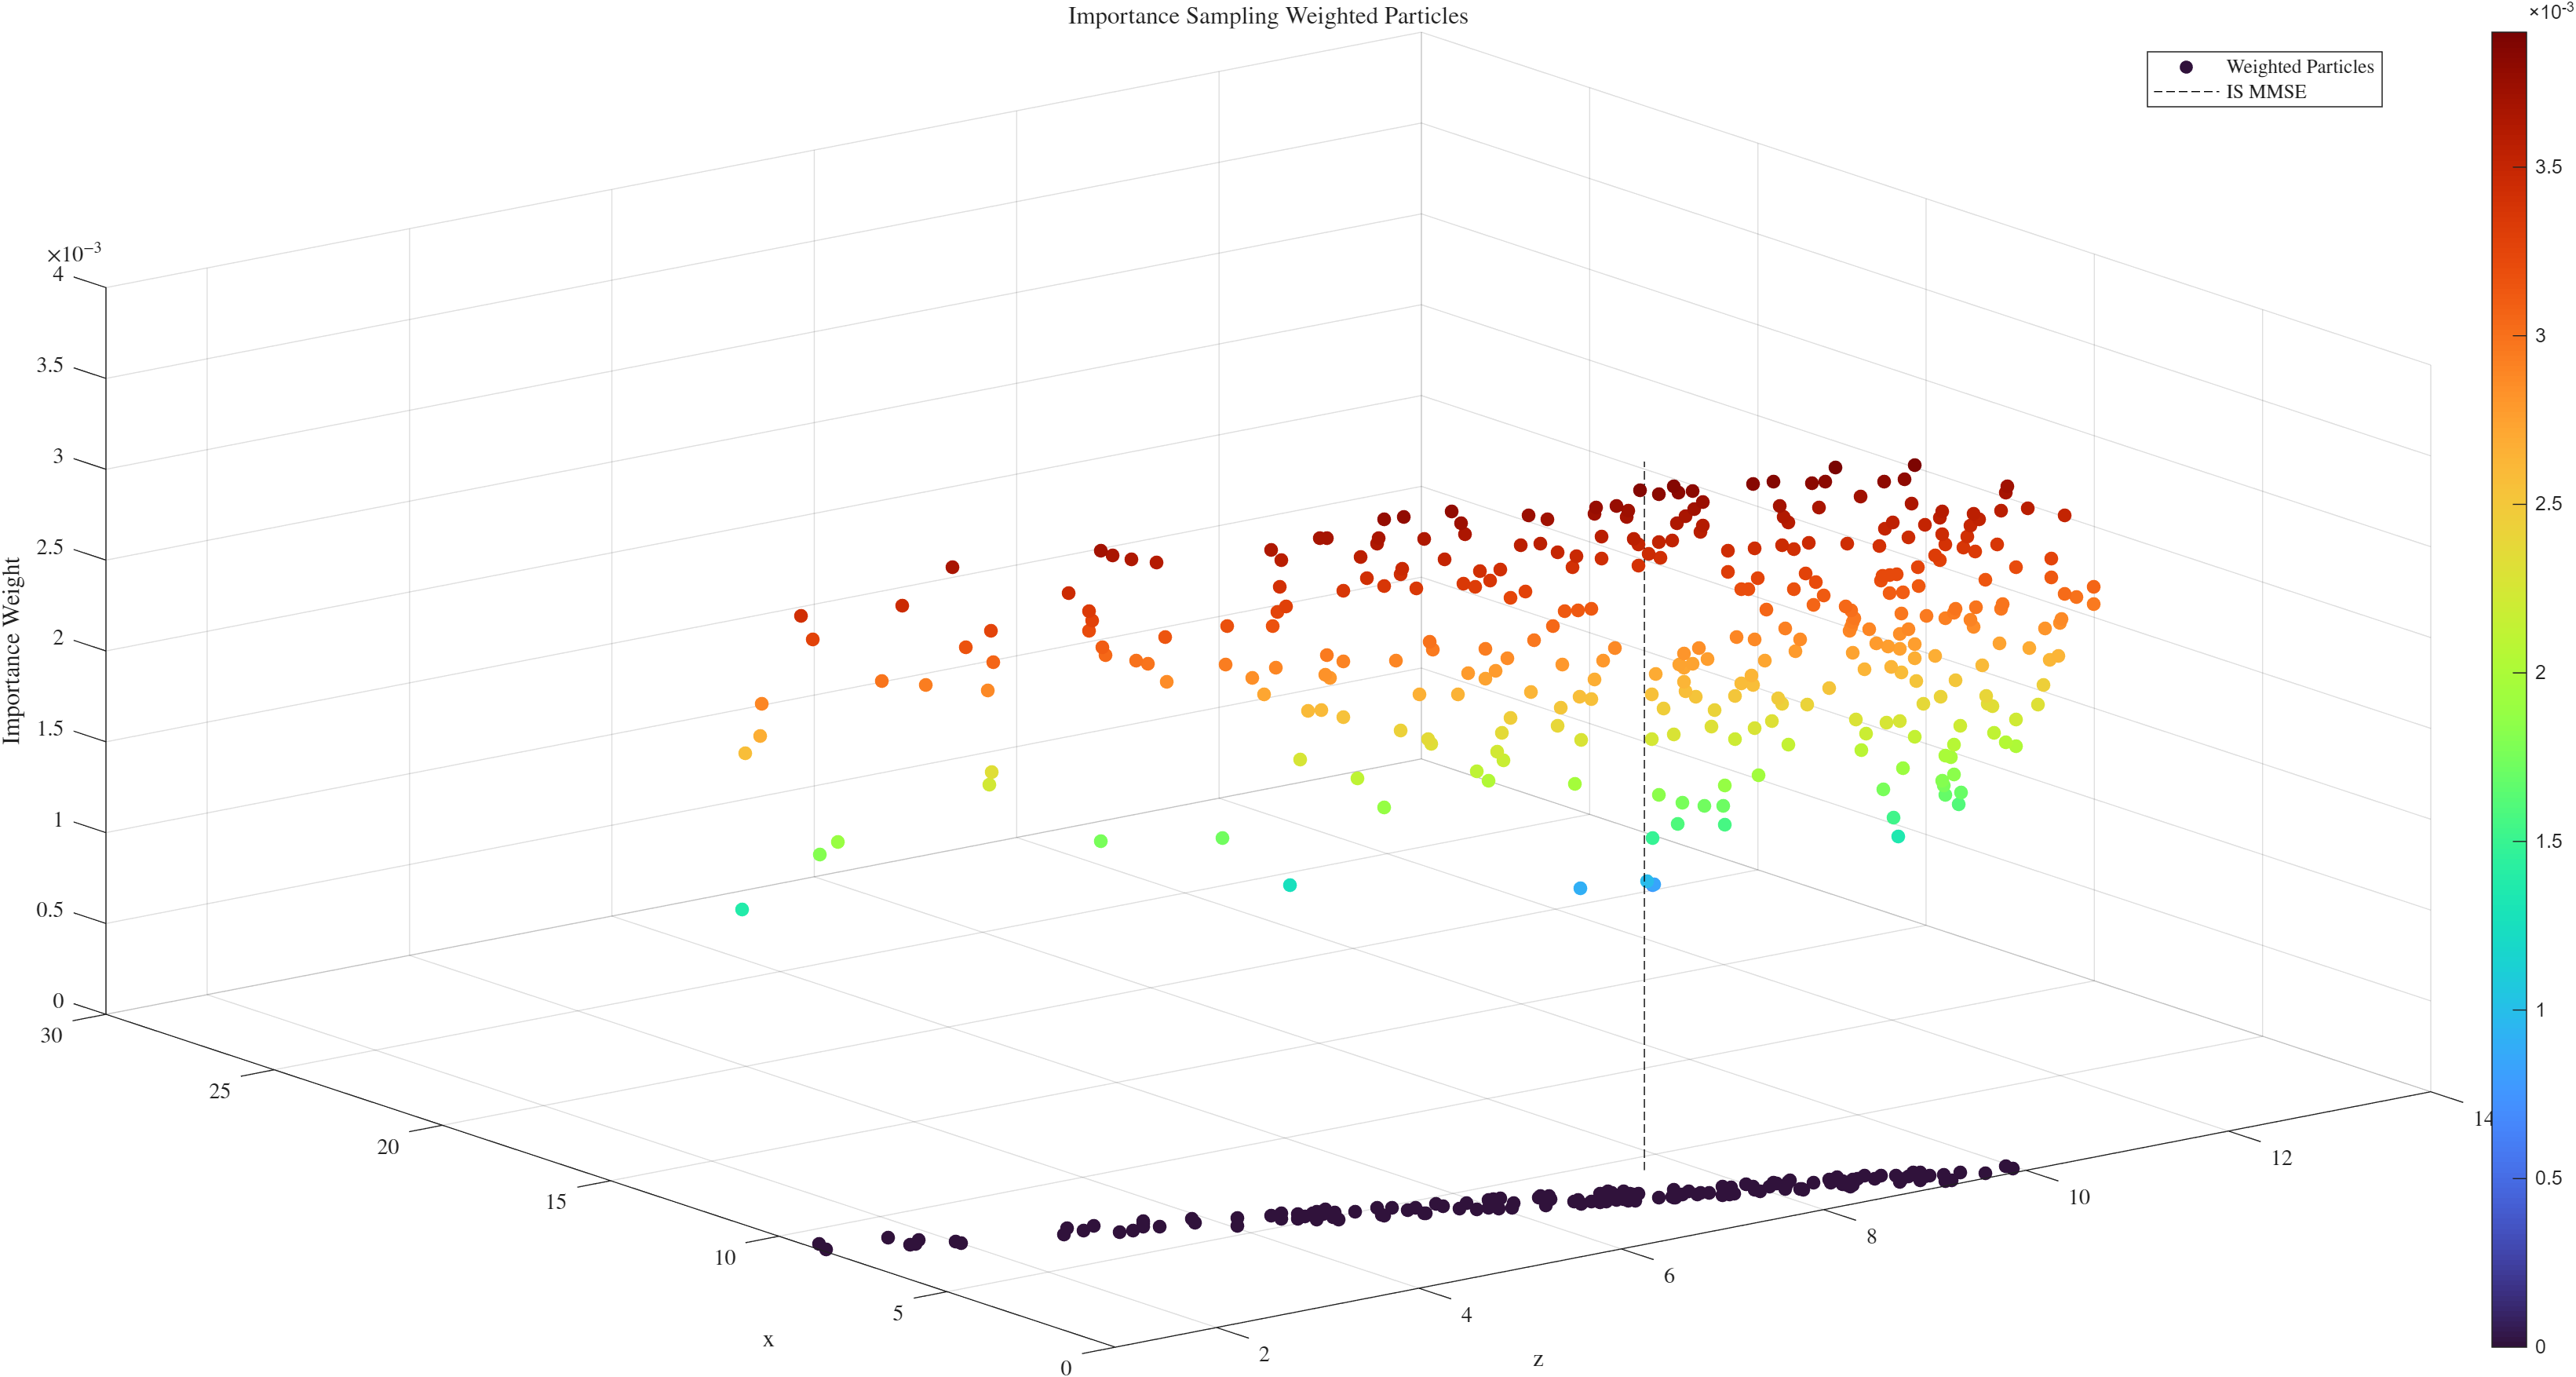
\includegraphics[width=\textwidth, height=\textheight, keepaspectratio]{IS.png}
            \caption{IS Estimate of $p(x,z \mid y_1, y_2,y_3)$}
            \label{fig:IS}
        \end{figure}
\end{enumerate}

\subsection{Code For Problem 1}

\begin{lstlisting}[style = matlab]
clear; clc; close all

rng(500)
%% Define grid space + paramters

dx = 0.05;
x = 1:dx:14;
z = dx:dx:30;
a = 2;
b = 2;

Nx = length(x);
Nz = length(z);
%% Define prior grid dist

px = zeros(1,Nx);
px(x >= 1 & x <= 11) = 1/(11-1);

pz = (1/(b^a * gamma(a))) .* (z.^(a-1)) .* exp(-z./b);

P = zeros(Nx,Nz);

for i = 1:Nx
    for j = 1:Nz
        P(i,j) = px(i) * pz(j);
    end
end

P = P / sum(P(:));

[X,Z] = meshgrid(z,x);

figure
surf(X,Z,P,'DisplayName','Prior')
xlabel('z')
ylabel('x')
zlabel('p(x,z)')
title('Joint Prior Distribution p(x,z)')
shading interp
legend('Location','best')

%% Posterior Bayes Update

y = [91.56, 70.43, 108.67];
Ny = 3;

L = likelihood(y(1),x,z);

figure
surf(X,Z,L,'DisplayName','Likelihood')
xlabel('z')
ylabel('x')
zlabel('p(y|x,z)')
title('Likelihood Dist p(y|x,z)')
shading interp
legend('Location','best')

for i = 1:Ny
    Posterior = BayesUpdate(y(i),x,z,P, true,i);
    P = Posterior;
    MAP = getMAP(P,x,z);
    MMSE = getMMSE(P,x,z);
end

%% IS

px = zeros(1,Nx);
px(x >= 1 & x <= 11) = 1/(11-1);

pz = (1/(b^a * gamma(a))) .* (z.^(a-1)) .* exp(-z./b);

P = zeros(Nx,Nz);

for i = 1:Nx
    for j = 1:Nz
        P(i,j) = px(i) * pz(j);
    end
end

for i = 1:Ny-1
    Posterior = BayesUpdate(y(i),x,z,P, false,i);
    P = Posterior;
    MAP = getMAP(P,x,z);
    MMSE = getMMSE(P,x,z);
end

Ns = 500; % Sample Count

% Sample from prior
cdf_prior = cumsum(P(:));
random_values = rand(Ns, 1);
sample_indices = arrayfun(@(t) find(cdf_prior >= t, 1, 'first'), random_values);
[row_indices, col_indices] = ind2sub(size(P), sample_indices);

xi = x(row_indices);
zi = z(col_indices);

w = zeros(1,500);

for i = 1:Ns

%w(i) = likelihood(y(1),xi(i),zi(i))*likelihood(y(2),xi(i),zi(i))*likelihood(y(3),xi(i),zi(i));
w(i) = likelihood(y(3),xi(i),zi(i));

end

w = w./sum(w); % Normalize

% MMSE estimate
IS_MMSE = [0;0];
for i = 1:Ns
    IS_MMSE = IS_MMSE + w(i)*[zi(i);xi(i)];
end

figure; hold on
scatter3(xi, zi, w, 40, w, 'filled', 'DisplayName', 'Weighted Particles')
plot3([IS_MMSE(1) IS_MMSE(1)],[IS_MMSE(2) IS_MMSE(2)],[0 max(w)],'k--', 'DisplayName', 'IS MMSE')
xlim([1 14])
ylim([0 30])
xlabel('z')
ylabel('x')
zlabel('Importance Weight')
title('Importance Sampling Weighted Particles')

colorbar
colormap turbo
grid on
legend('Location','best')
view(3)
exportgraphics(gcf, "IS.png", 'Resolution', 200);

%% Helper Functions

function [L] = likelihood(y,x,z)

Nx = length(x);
Nz = length(z);
L = zeros(Nx,Nz);

for i = 1:Nx
    for j = 1:Nz
        % Out of bounds
        if y < x(i) || y > (x(i)+z(j))^2
            L(i,j) = 0;
            continue
        end

        L(i,j) = 1/((x(i)+z(j))^2-x(i));
    end
end
    
    
end

function [Posterior] = BayesUpdate(y,x,z,Prior, PLOT,i)

L = likelihood(y,x,z);

Posterior = Prior.*L;
fprintf("Value of Marginal P(y_1:N) = %d for meas 1:%i \n",sum(Posterior(:)),i)
Posterior = Posterior./(sum(Posterior(:)));



if PLOT
    MAP = getMAP(Posterior,x,z);
    MMSE = getMMSE(Posterior,x,z);
    [X,Z] = meshgrid(z,x);
    figure
    hold on
    surf(Z,X,Posterior,'DisplayName','Posterior')
    scatter3(MAP(1),MAP(2),MAP(3),'rx','DisplayName','MAP')
    plot3([MMSE(1) MMSE(1)],[MMSE(2) MMSE(2)],[0 MAP(3)],'k--','DisplayName','MMSE')
    xlabel('x')
    ylabel('z')
    zlabel('p(x,z|y)')
    title(sprintf('p(x,z | y_1...y_%d)',i))    
    shading interp
    legend('Location','best')
    view(3)
    exportgraphics(gcf, sprintf('Measurment_%d',i) +  ".png", 'Resolution', 200);
end
end

function [MAP] = getMAP(P,x,z)

    [peak,idx] = max(P(:));
    [row, col] = ind2sub(size(P), idx);
    [X,Z] = meshgrid(z,x);
    map_z = X(row,col);
    map_x = Z(row,col);

    MAP = [map_z;map_x;peak];

end

function [MMSE] = getMMSE(P,x,z)
[X,Z] = meshgrid(z,x);

z_mmse = sum(sum(P .* X));
x_mmse = sum(sum(P .* Z));

[~, ix] = min(abs(x - x_mmse));
[~, iz] = min(abs(z - z_mmse));

MMSE = [z_mmse; x_mmse; P(ix,iz)];

end

\end{lstlisting}
% =====================================================
\section{}

\begin{enumerate}[label = \alph*)]
    \item 
        Given the state index transition probabilities, we can compile all of the transition information into a matrix $T \in \mathbb{R}^{N_x \times N_x}$ with
        \[
            T_{ij} = P(\zeta_{k+1}=i \mid \zeta_k=j),
            \qquad
            \rho_{k+1} = T \rho_k.
        \]
        Therefore, column $j$ corresponds to the current state $\zeta_k=j$, while row $i$ corresponds to the propagated state $\zeta_{k+1}=i$. 
        \[
        T =
        \begin{bmatrix}
        0.1 & 0.2 & 0   & 0   & \cdots & 0   & 0 \\
        0.9 & 0.3 & 0.2 & 0   & \cdots & 0   & 0 \\
        0   & 0.5 & 0.3 & 0.2 & \ddots & \vdots & \vdots \\
        0   & 0   & 0.5 & 0.3 & \ddots & 0   & 0 \\
        \vdots & \vdots & \ddots & \ddots & \ddots & 0.2 & 0 \\
        0   & 0   & \cdots & 0   & 0.5 & 0.3 & 0.9 \\
        0   & 0   & \cdots & 0   & 0   & 0.5 & 0.1
        \end{bmatrix}.
        \]

        A stationary distribution $\rho^-_\infty$ such that $\rho^-_\infty = T \rho^-_\infty$ will exist if the square matrix $T$ has an eigenvalue $\lambda = 1$. In such case, the matrix eigenvalue equation becomes
        \(T\vec{v} = \vec{v}\) where $\vec{v}$ is the eigenvector corresponding to $\lambda = 1$. By definition of a stationary distribution, the eigenvector corresponding to $\lambda = 1$ is our stationary distribution. 
        Since $T$ has an eigenvalue $\lambda = 1$, there exists a stationary distribution $\rho^-_\infty$.

    \item  
        To derive a general expression for $\rho^-_k$ in terms of $\rho^-_0$, we start with the following
        \begin{align*}
            \rho^-_1 &= T \rho^-_0 \\
            \rho^-_2 &= T \rho^-_1 = T T \rho^-_0 = T^2 \rho^-_0 \\ 
            \rho^-_3 &= T \rho^-_2 = T^3 \rho^-_0
        \end{align*}
        This can be generalized so that at time step k we have 
        \begin{align*}
            \rho^-_k = T^k \rho^-_0
        \end{align*}
        This distribution is plotted for $k = 10,50,180,300,600$ in figures \ref{fig:r10} - \ref{fig:r600}. $\rho^-_\infty$ is shown in figure \ref{fig:rinf}. We see that $\rho^-_{600}$ is identical to the stationary distribution, however figure \ref{fig:r300} 
        shows us that after approximatly 300 timesteps, $\rho^-$ gets very close to the stationary distribution.

        \begin{figure}[H]
            \centering

            \begin{subfigure}[t]{0.32\textwidth}
                \centering
                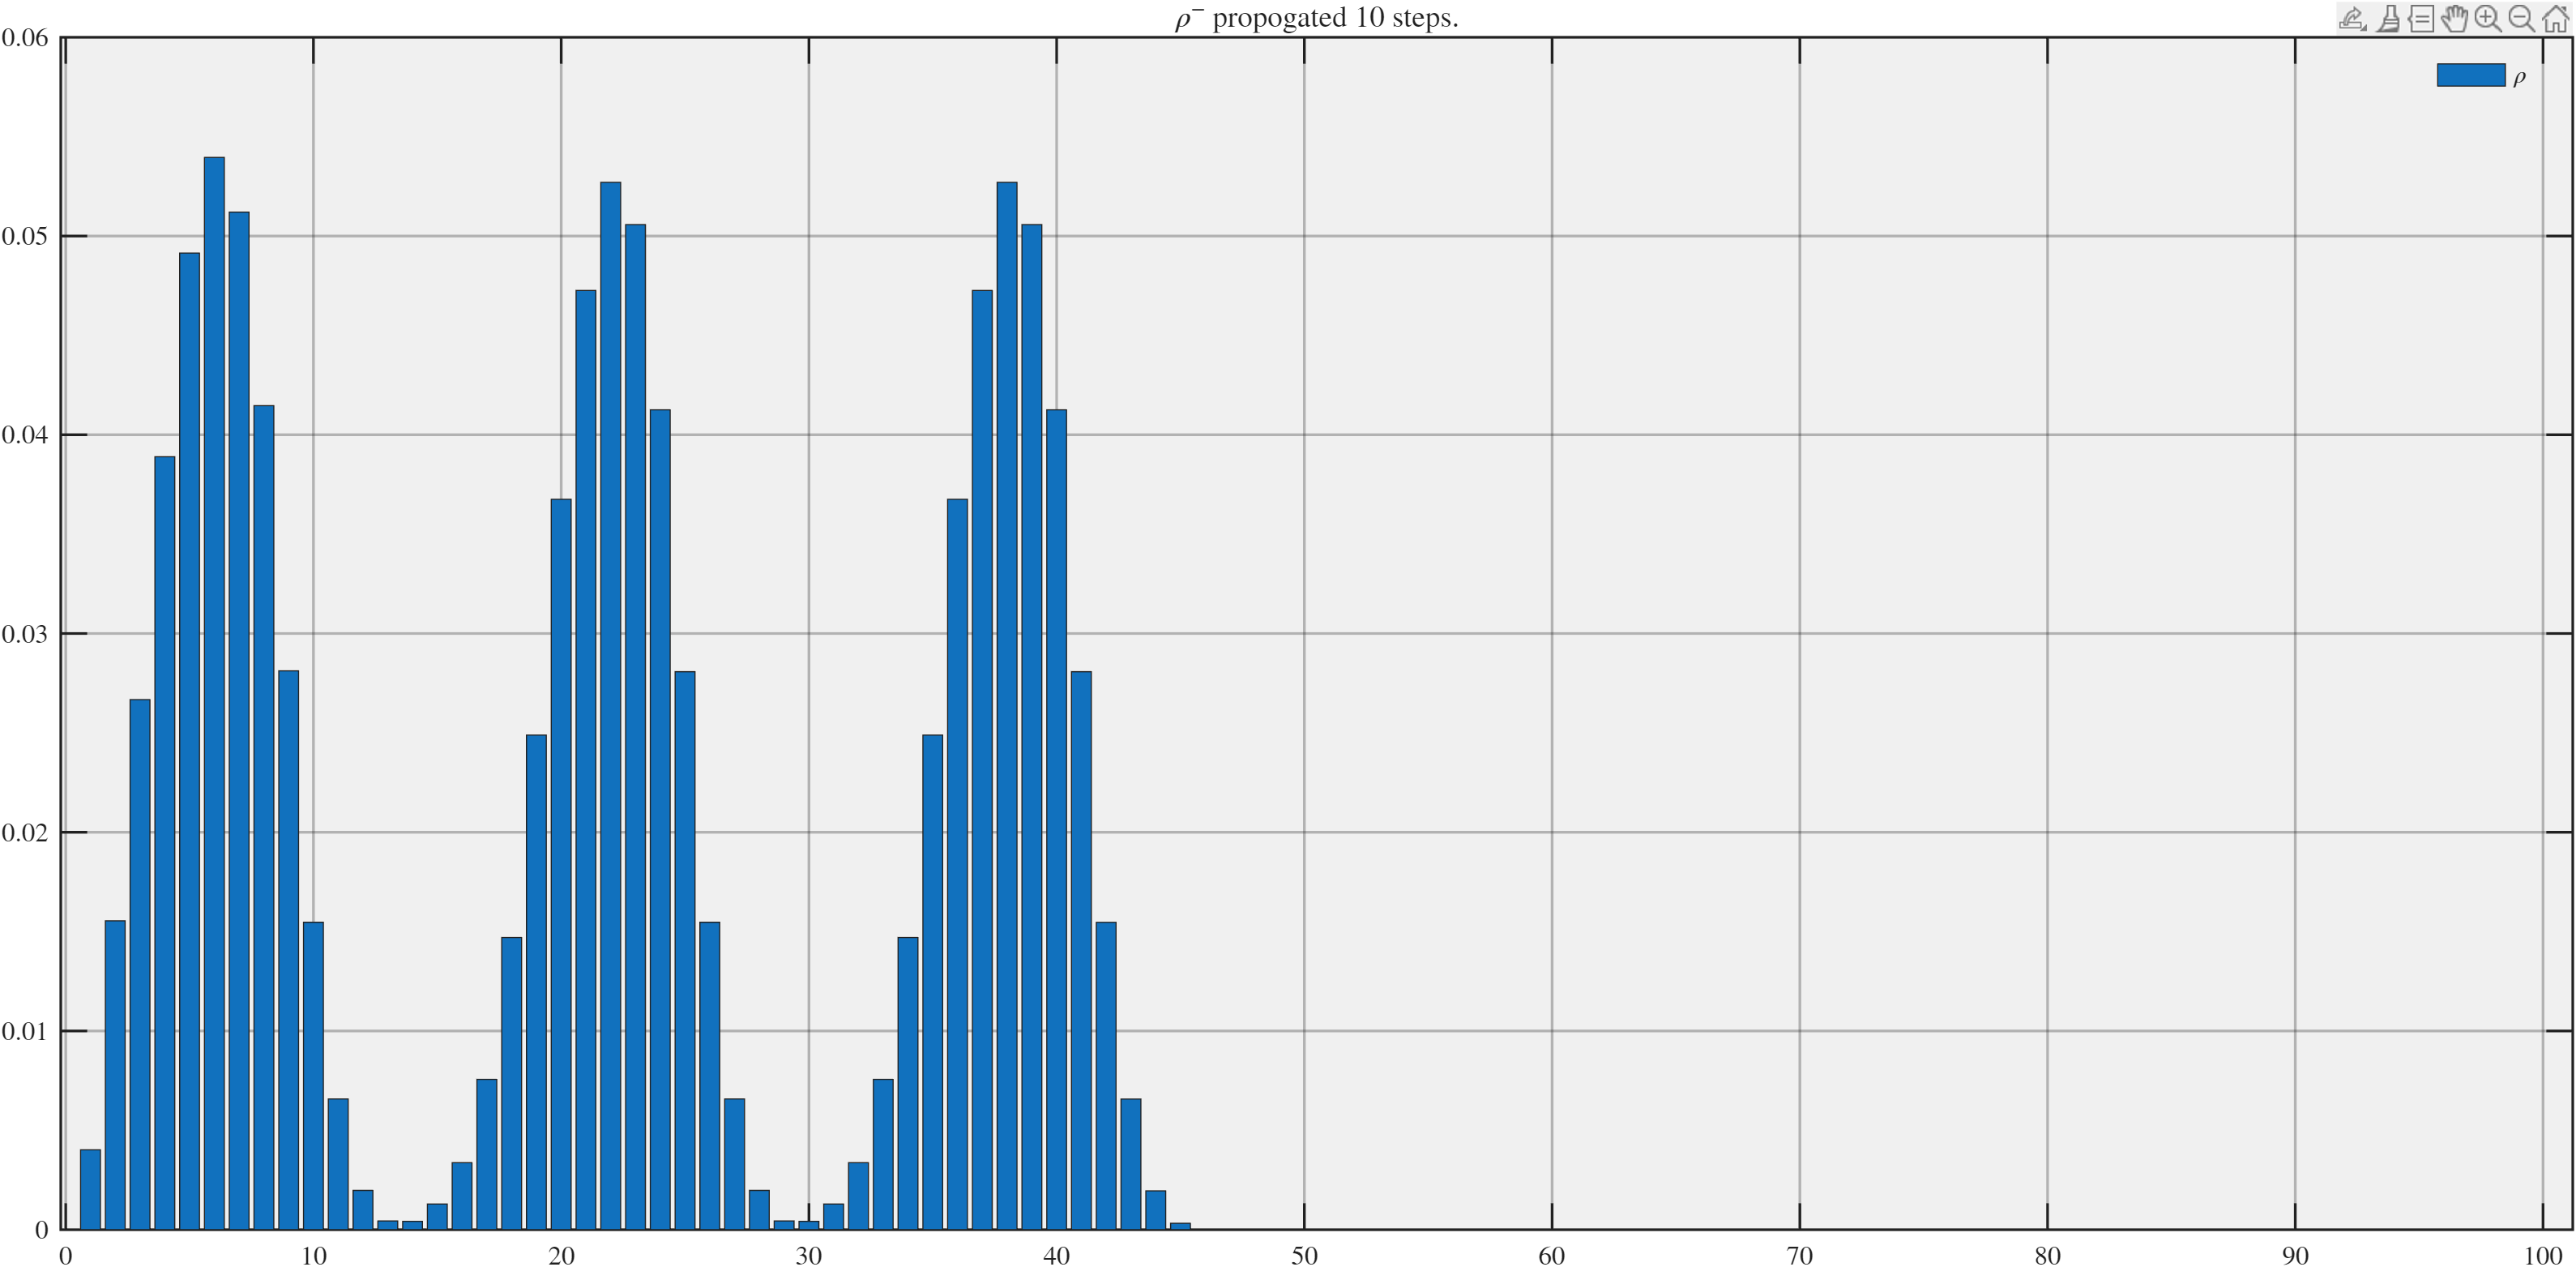
\includegraphics[width=\linewidth]{rho_propagated_010.png}
                \caption{$\rho^-_{10}$}
                \label{fig:r10}
            \end{subfigure}
            \hfill
            \begin{subfigure}[t]{0.32\textwidth}
                \centering
                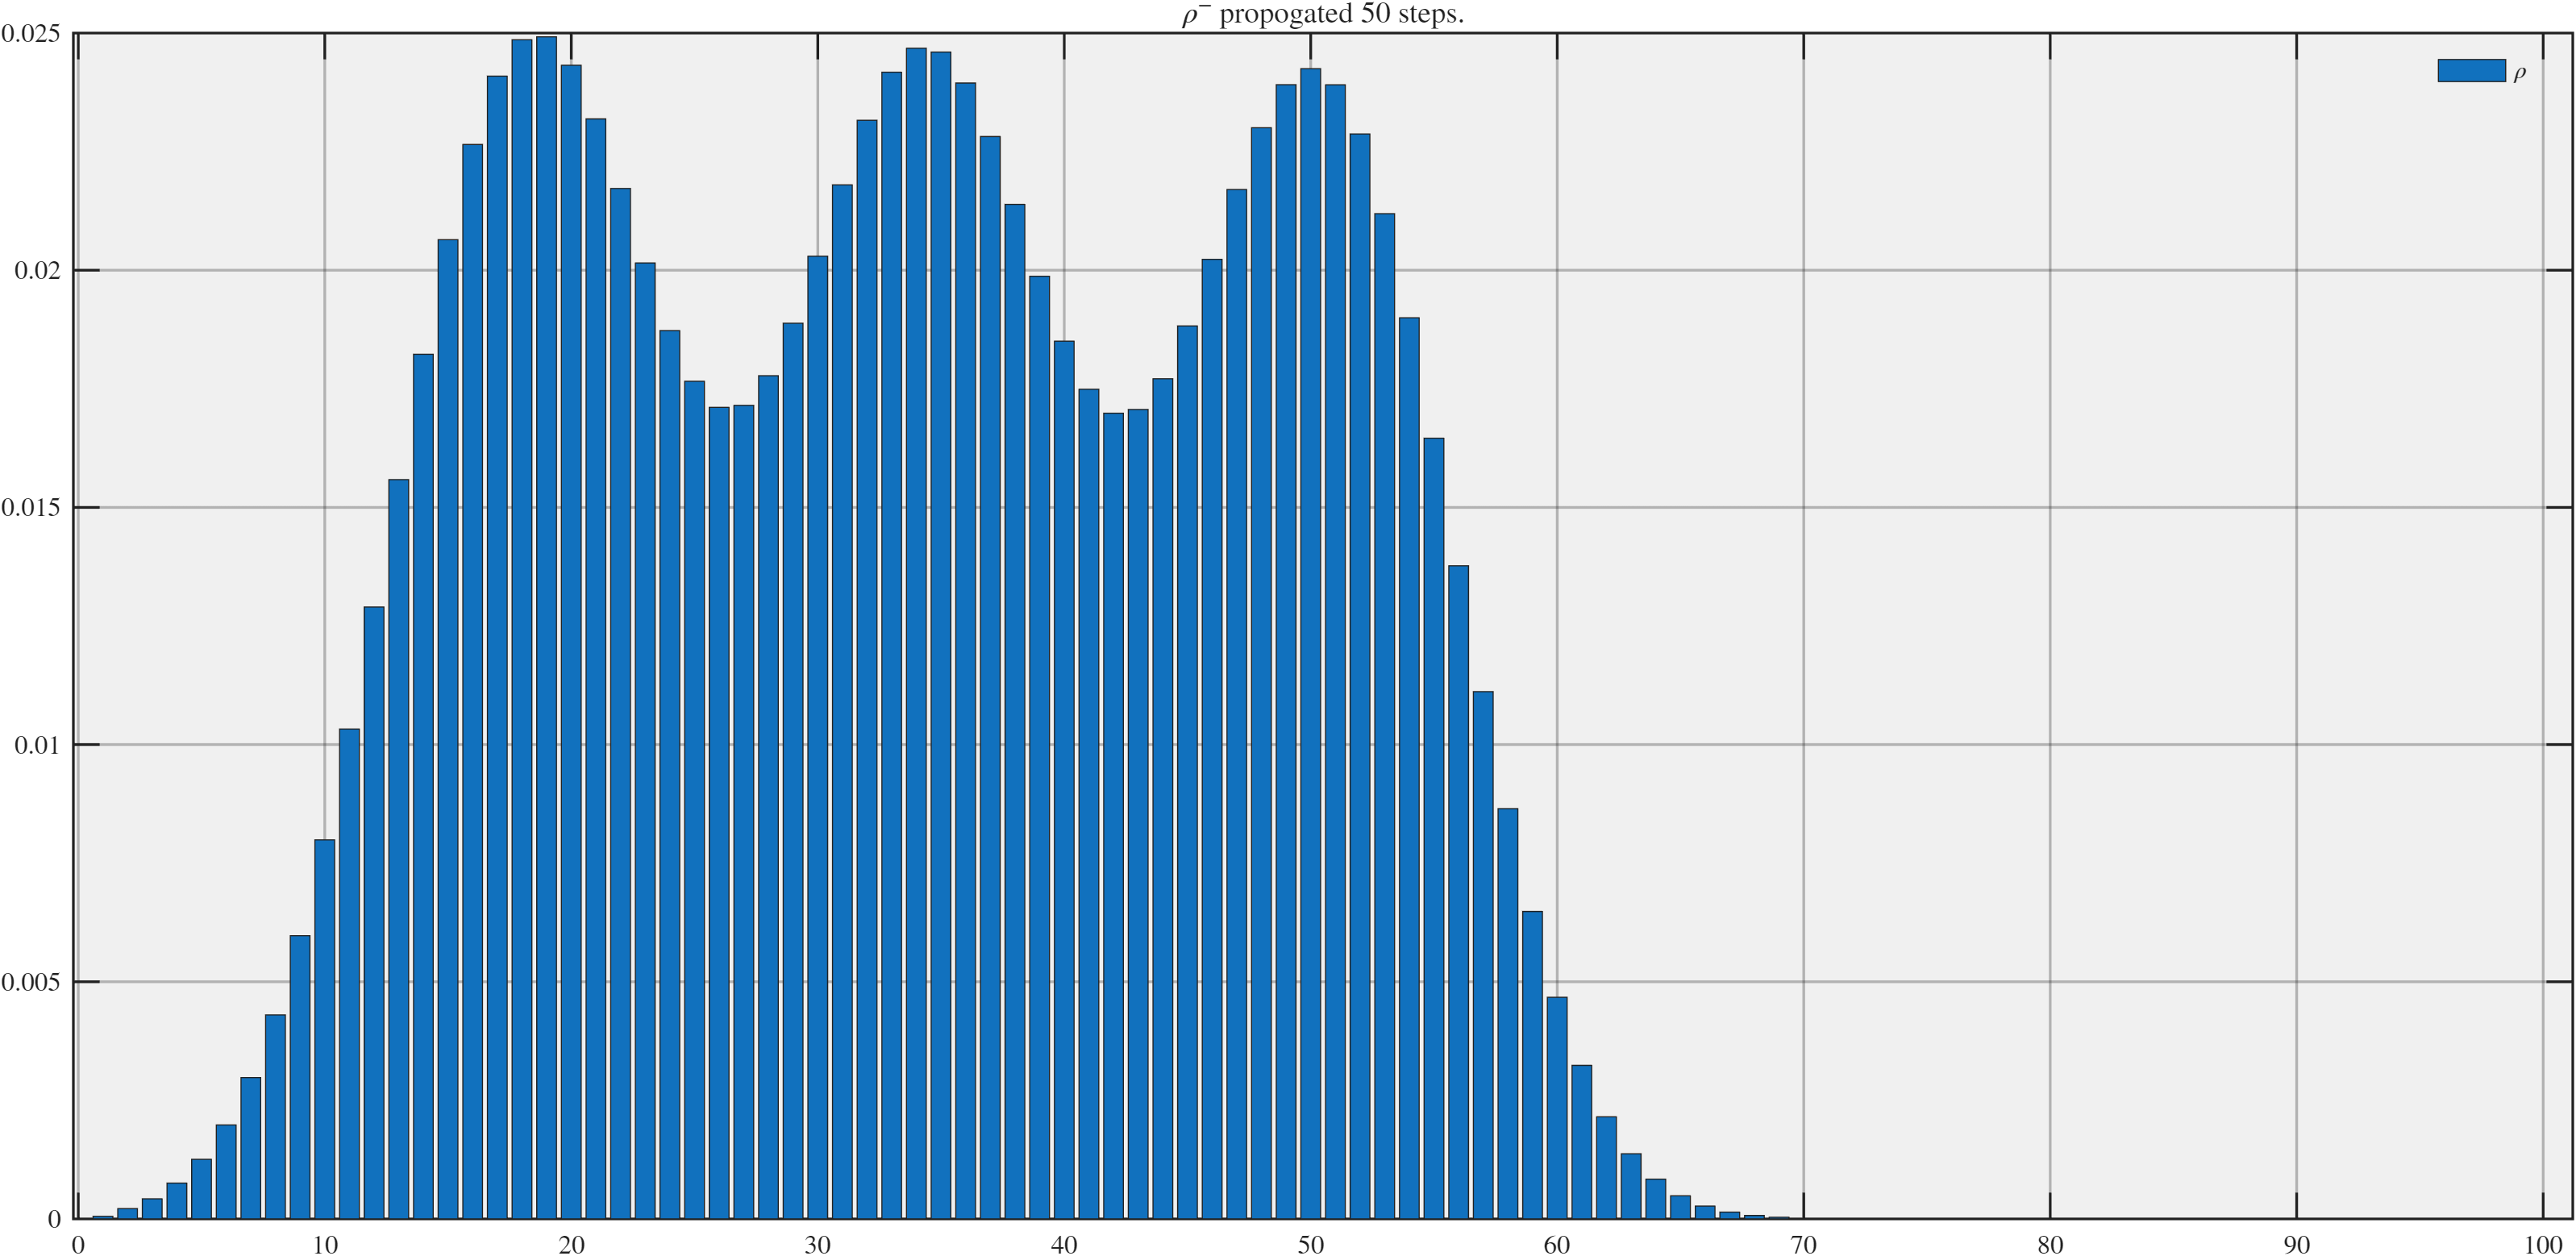
\includegraphics[width=\linewidth]{rho_propagated_050.png}
                \caption{$\rho^-_{50}$}
                \label{fig:r50}
            \end{subfigure}
            \hfill
            \begin{subfigure}[t]{0.32\textwidth}
                \centering
                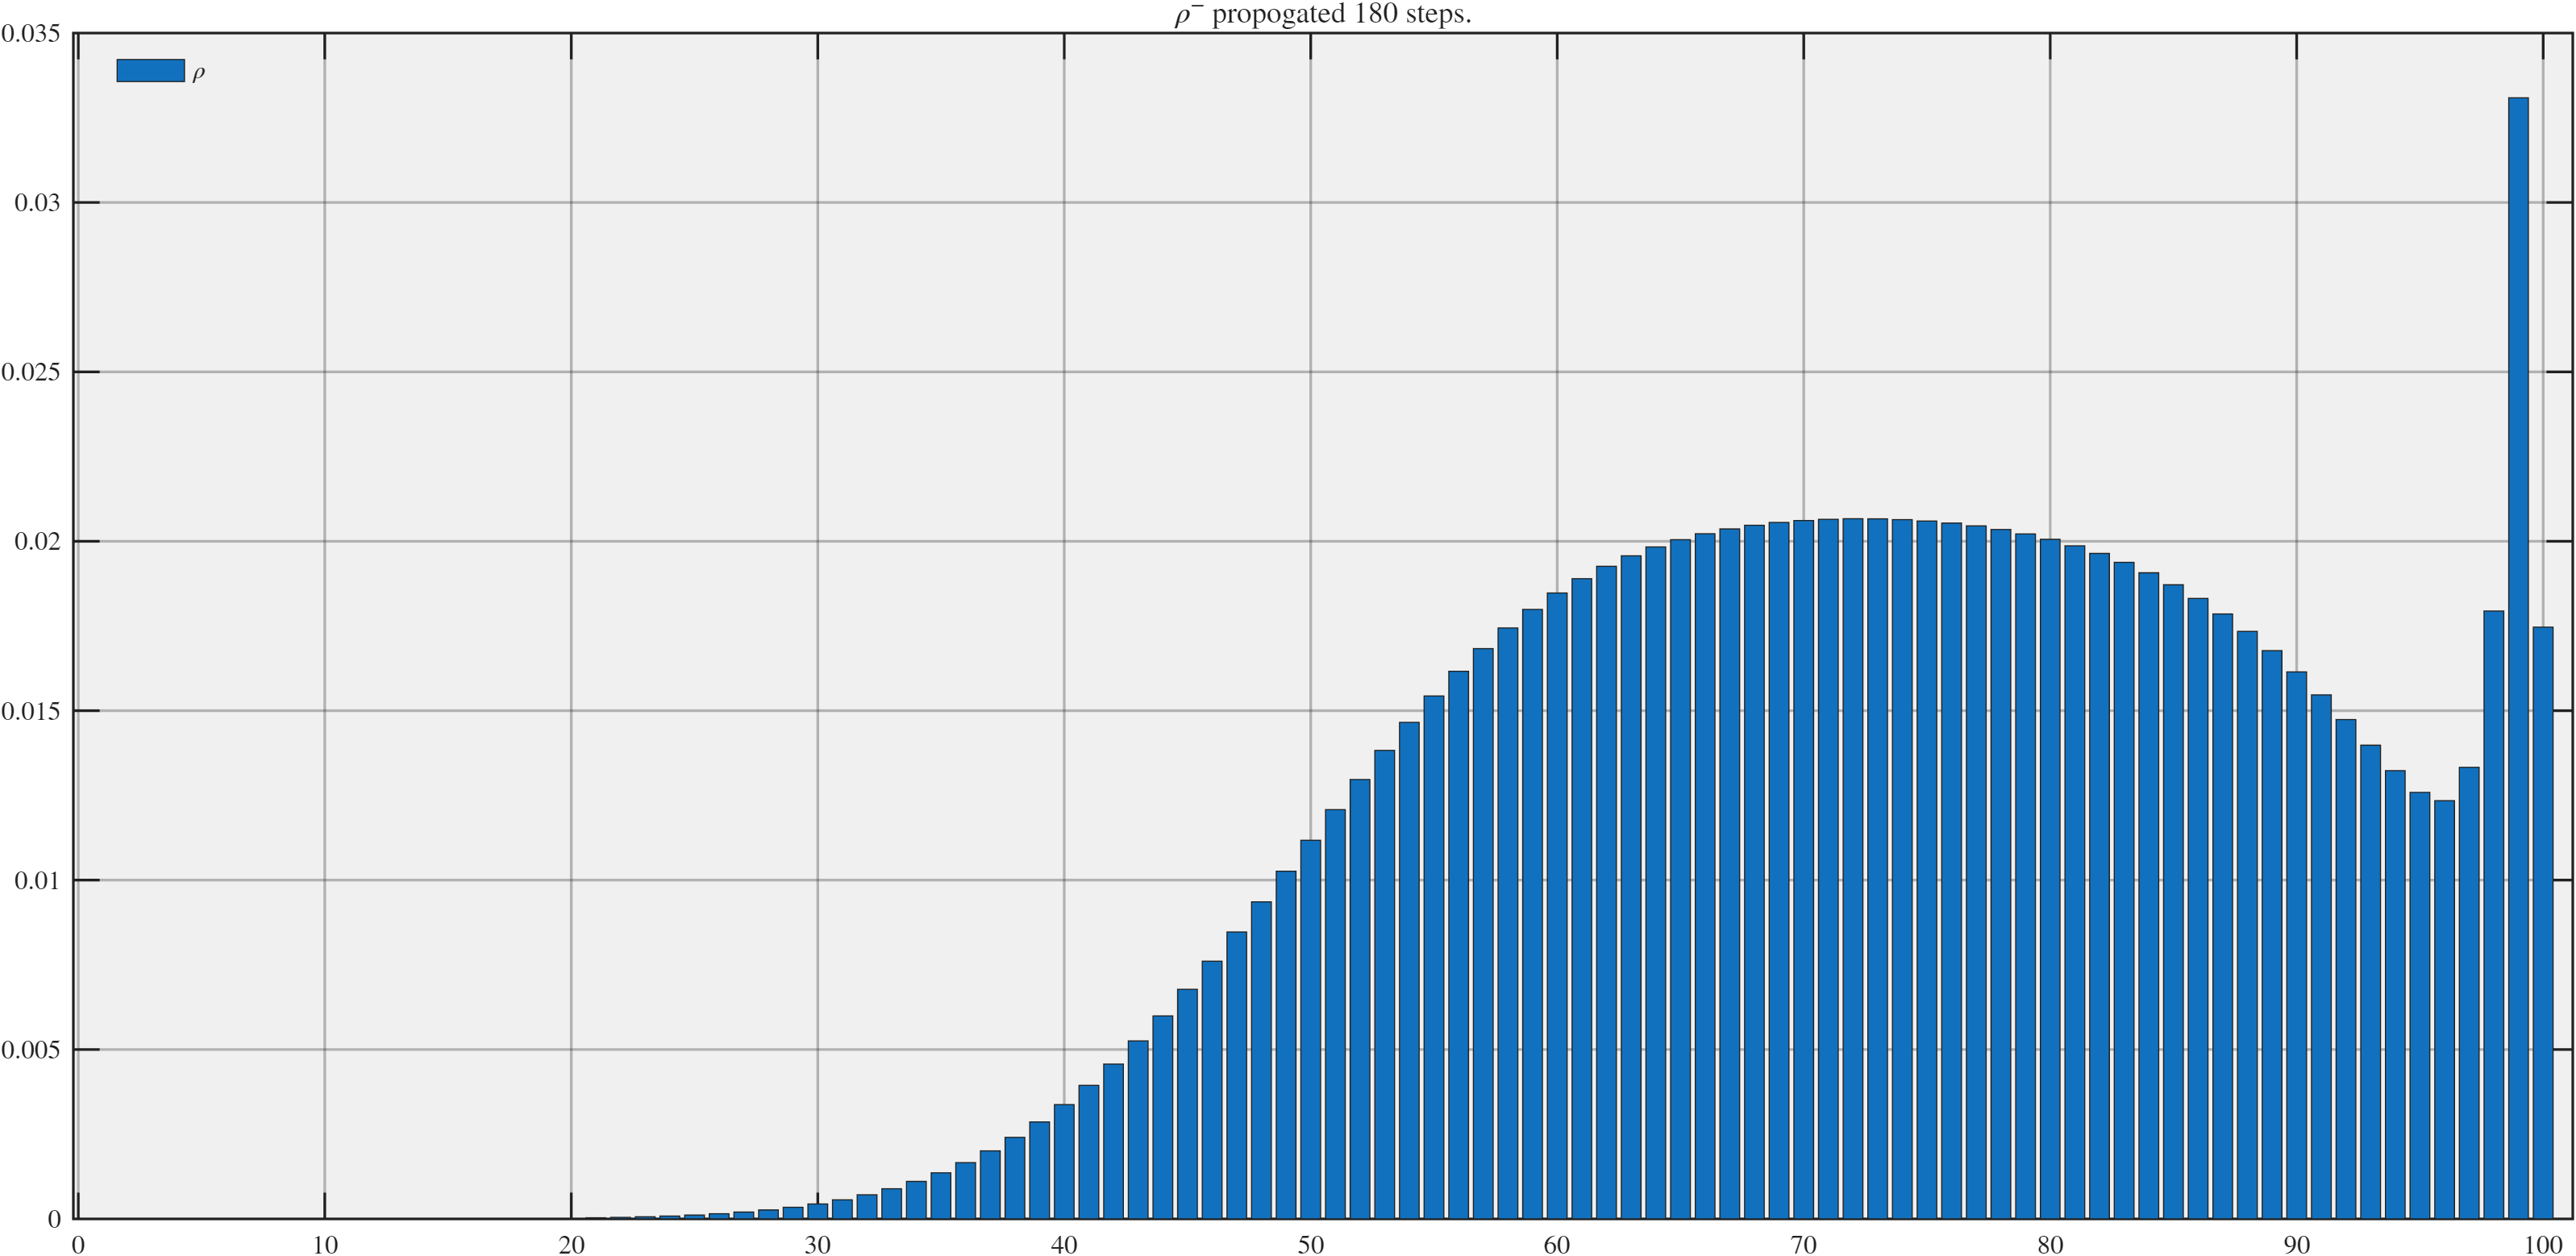
\includegraphics[width=\linewidth]{rho_propagated_180.png}
                \caption{$\rho^-_{180}$}
                \label{fig:r180}
            \end{subfigure}

            \vspace{0.6em}

            \begin{subfigure}[t]{0.32\textwidth}
                \centering
                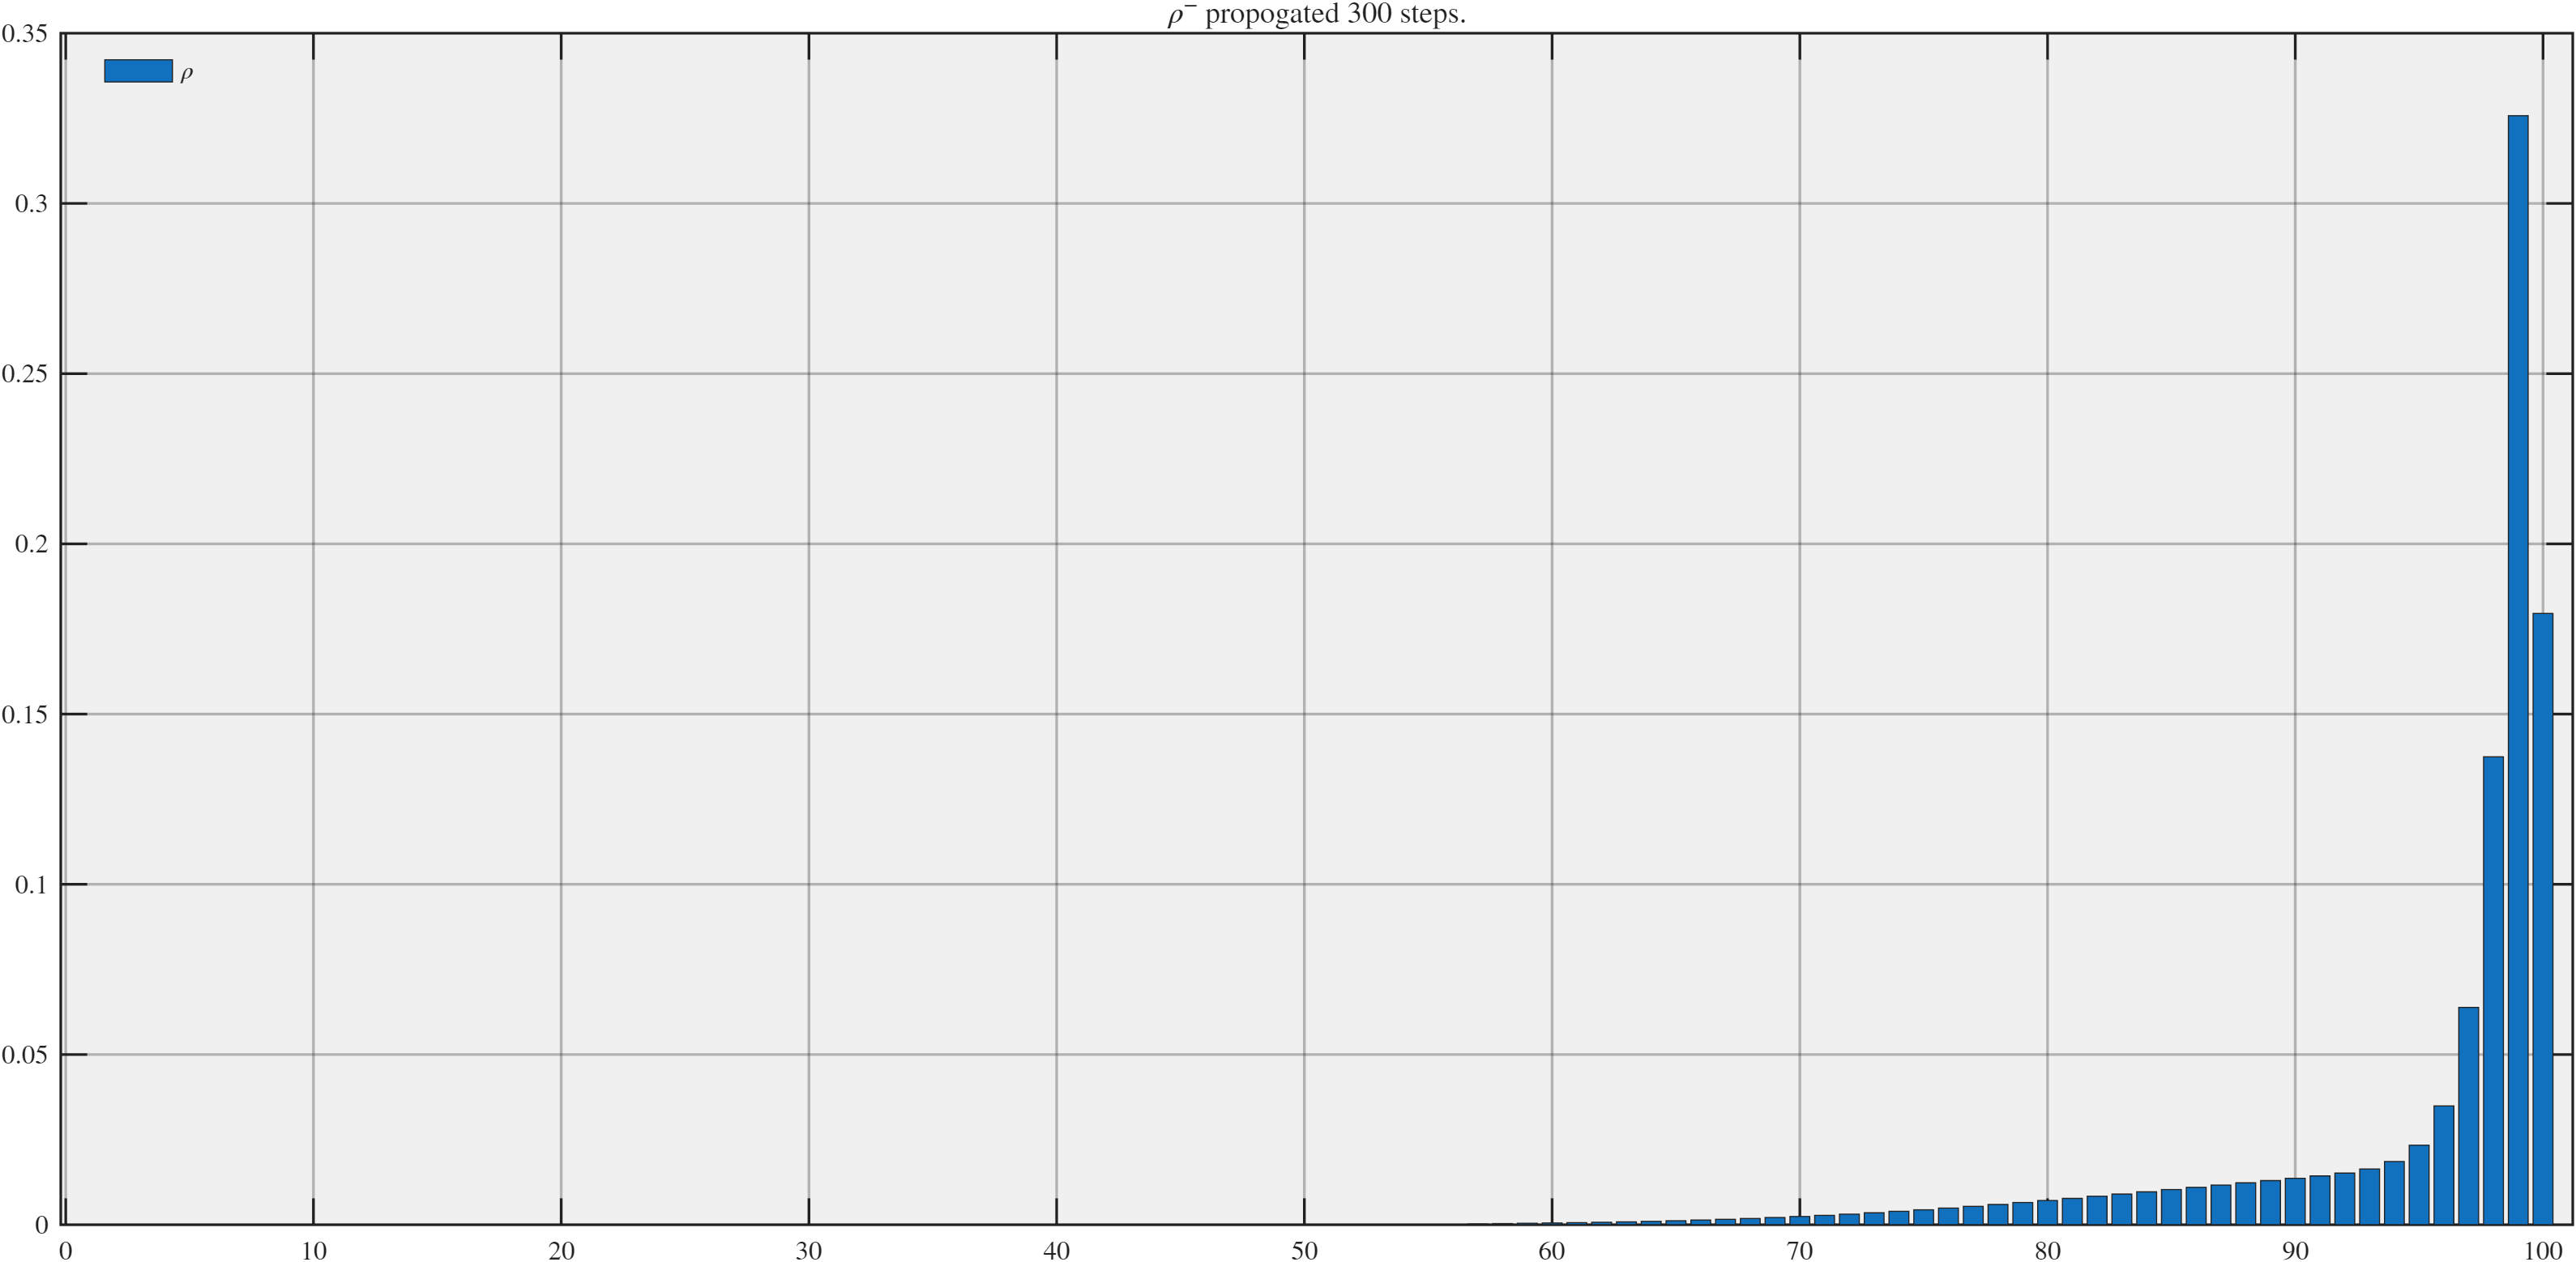
\includegraphics[width=\linewidth]{rho_propagated_300.png}
                \caption{$\rho^-_{300}$}
                \label{fig:r300}
            \end{subfigure}
            \hfill
            \begin{subfigure}[t]{0.32\textwidth}
                \centering
                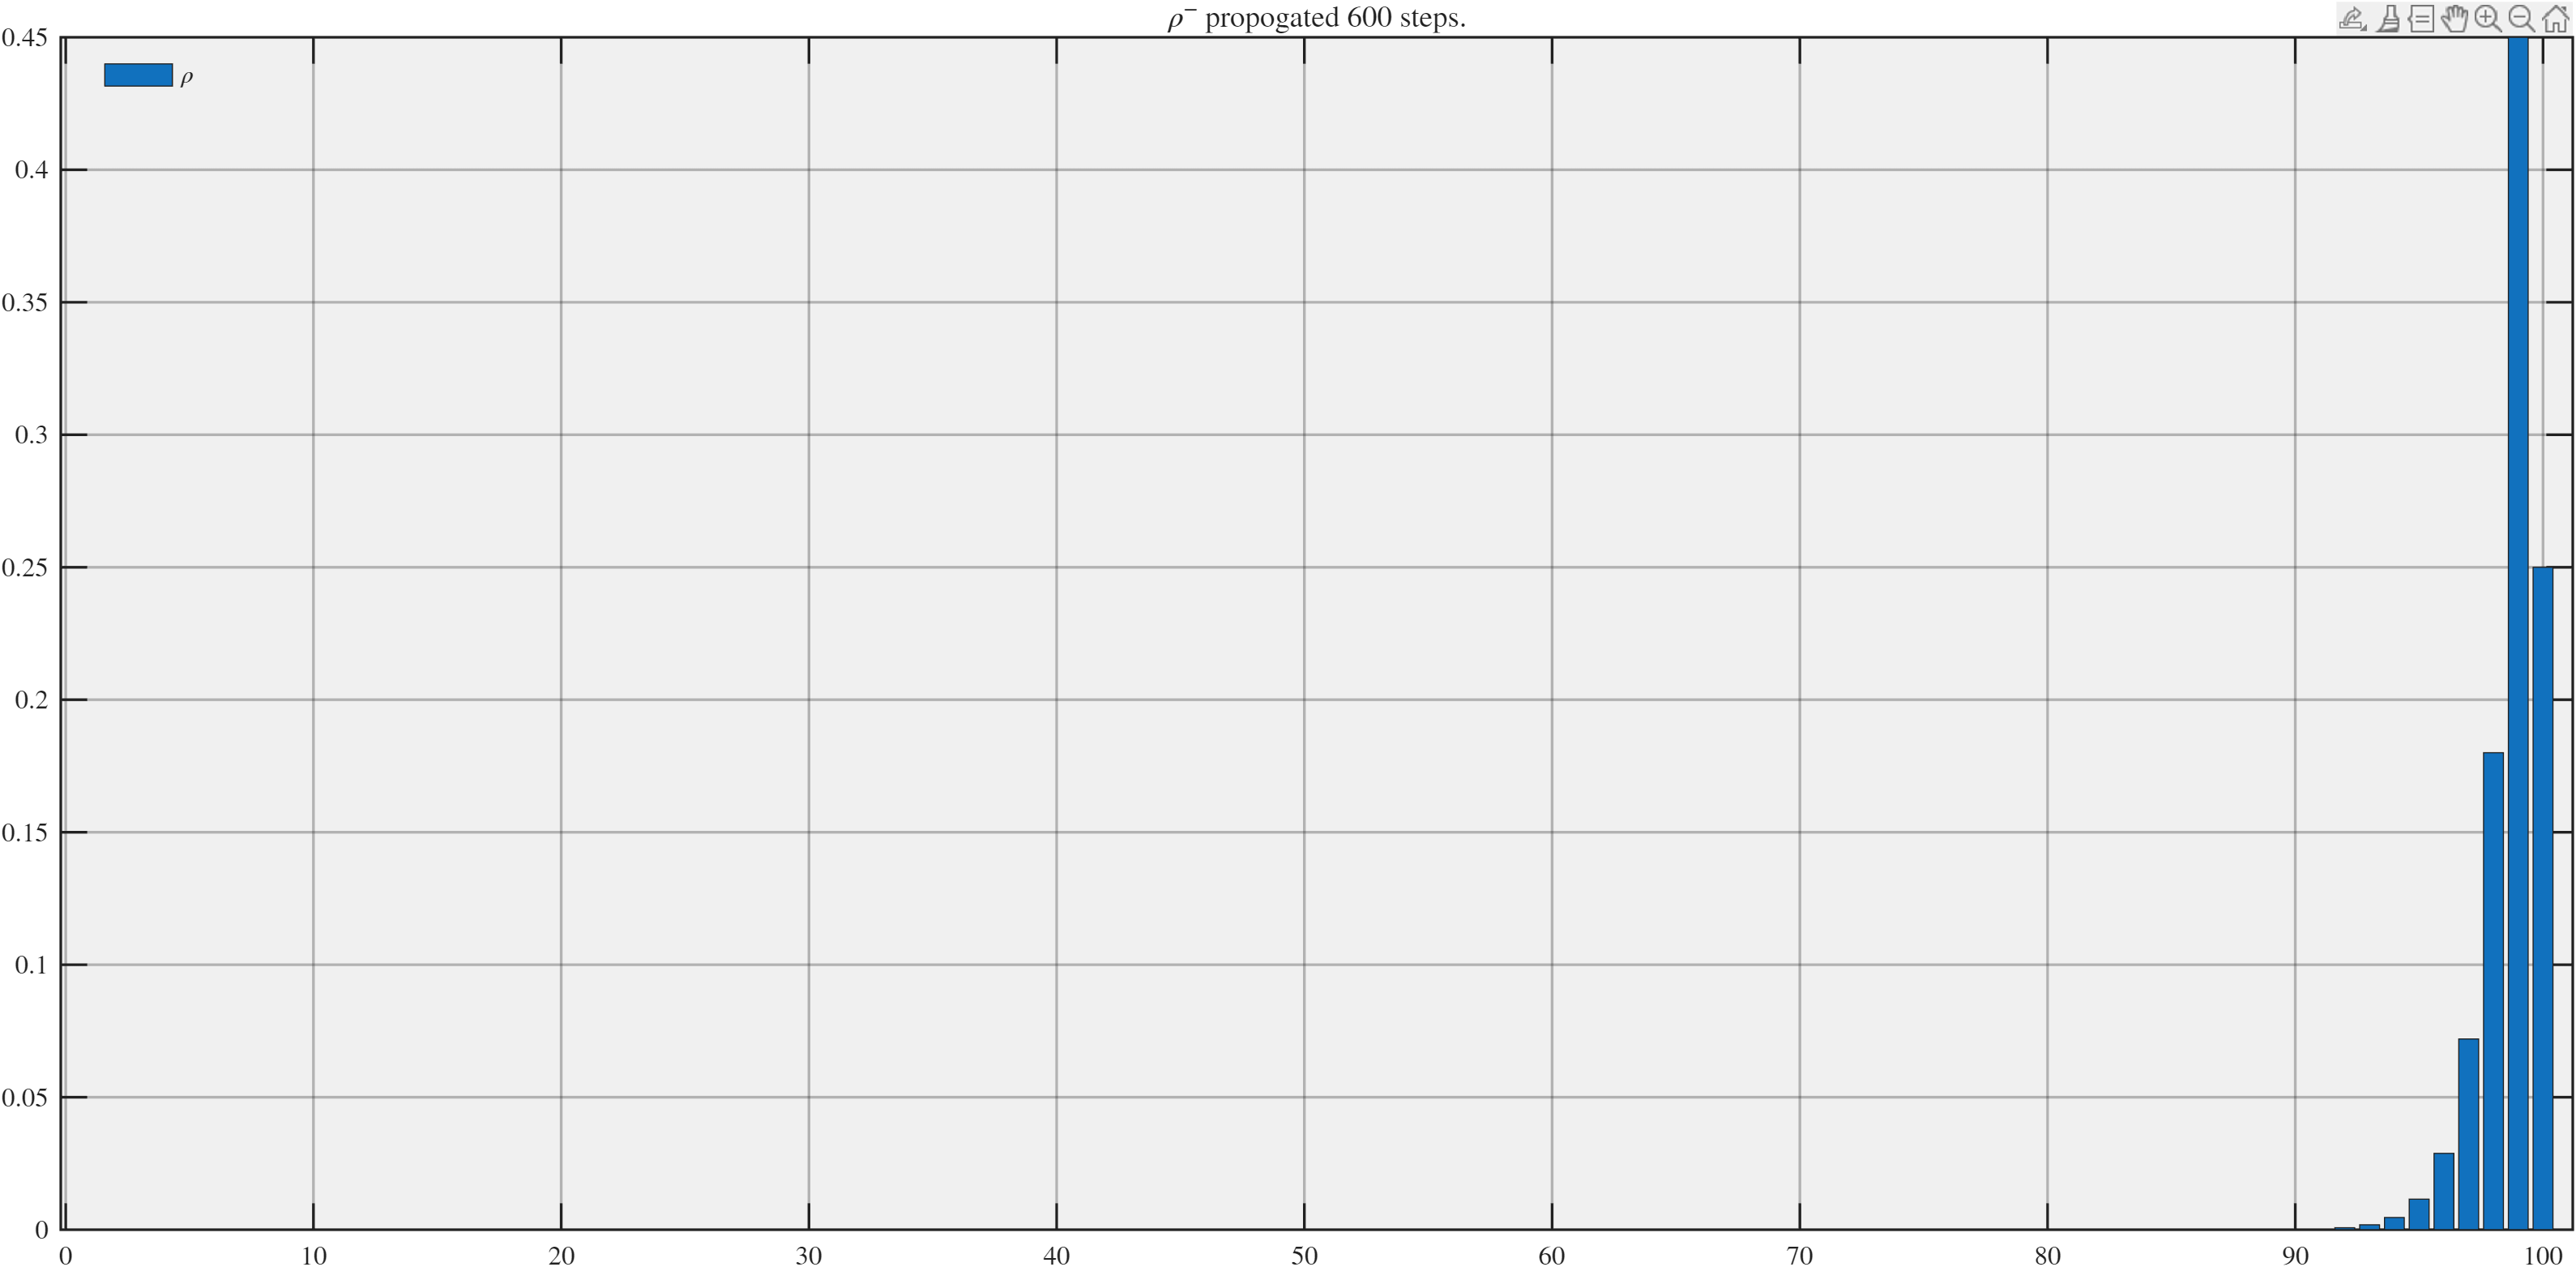
\includegraphics[width=\linewidth]{rho_propagated_600.png}
                \caption{$\rho^-_{600}$}
                \label{fig:r600}
            \end{subfigure}
            \hfill
            \begin{subfigure}[t]{0.32\textwidth}
                \centering
                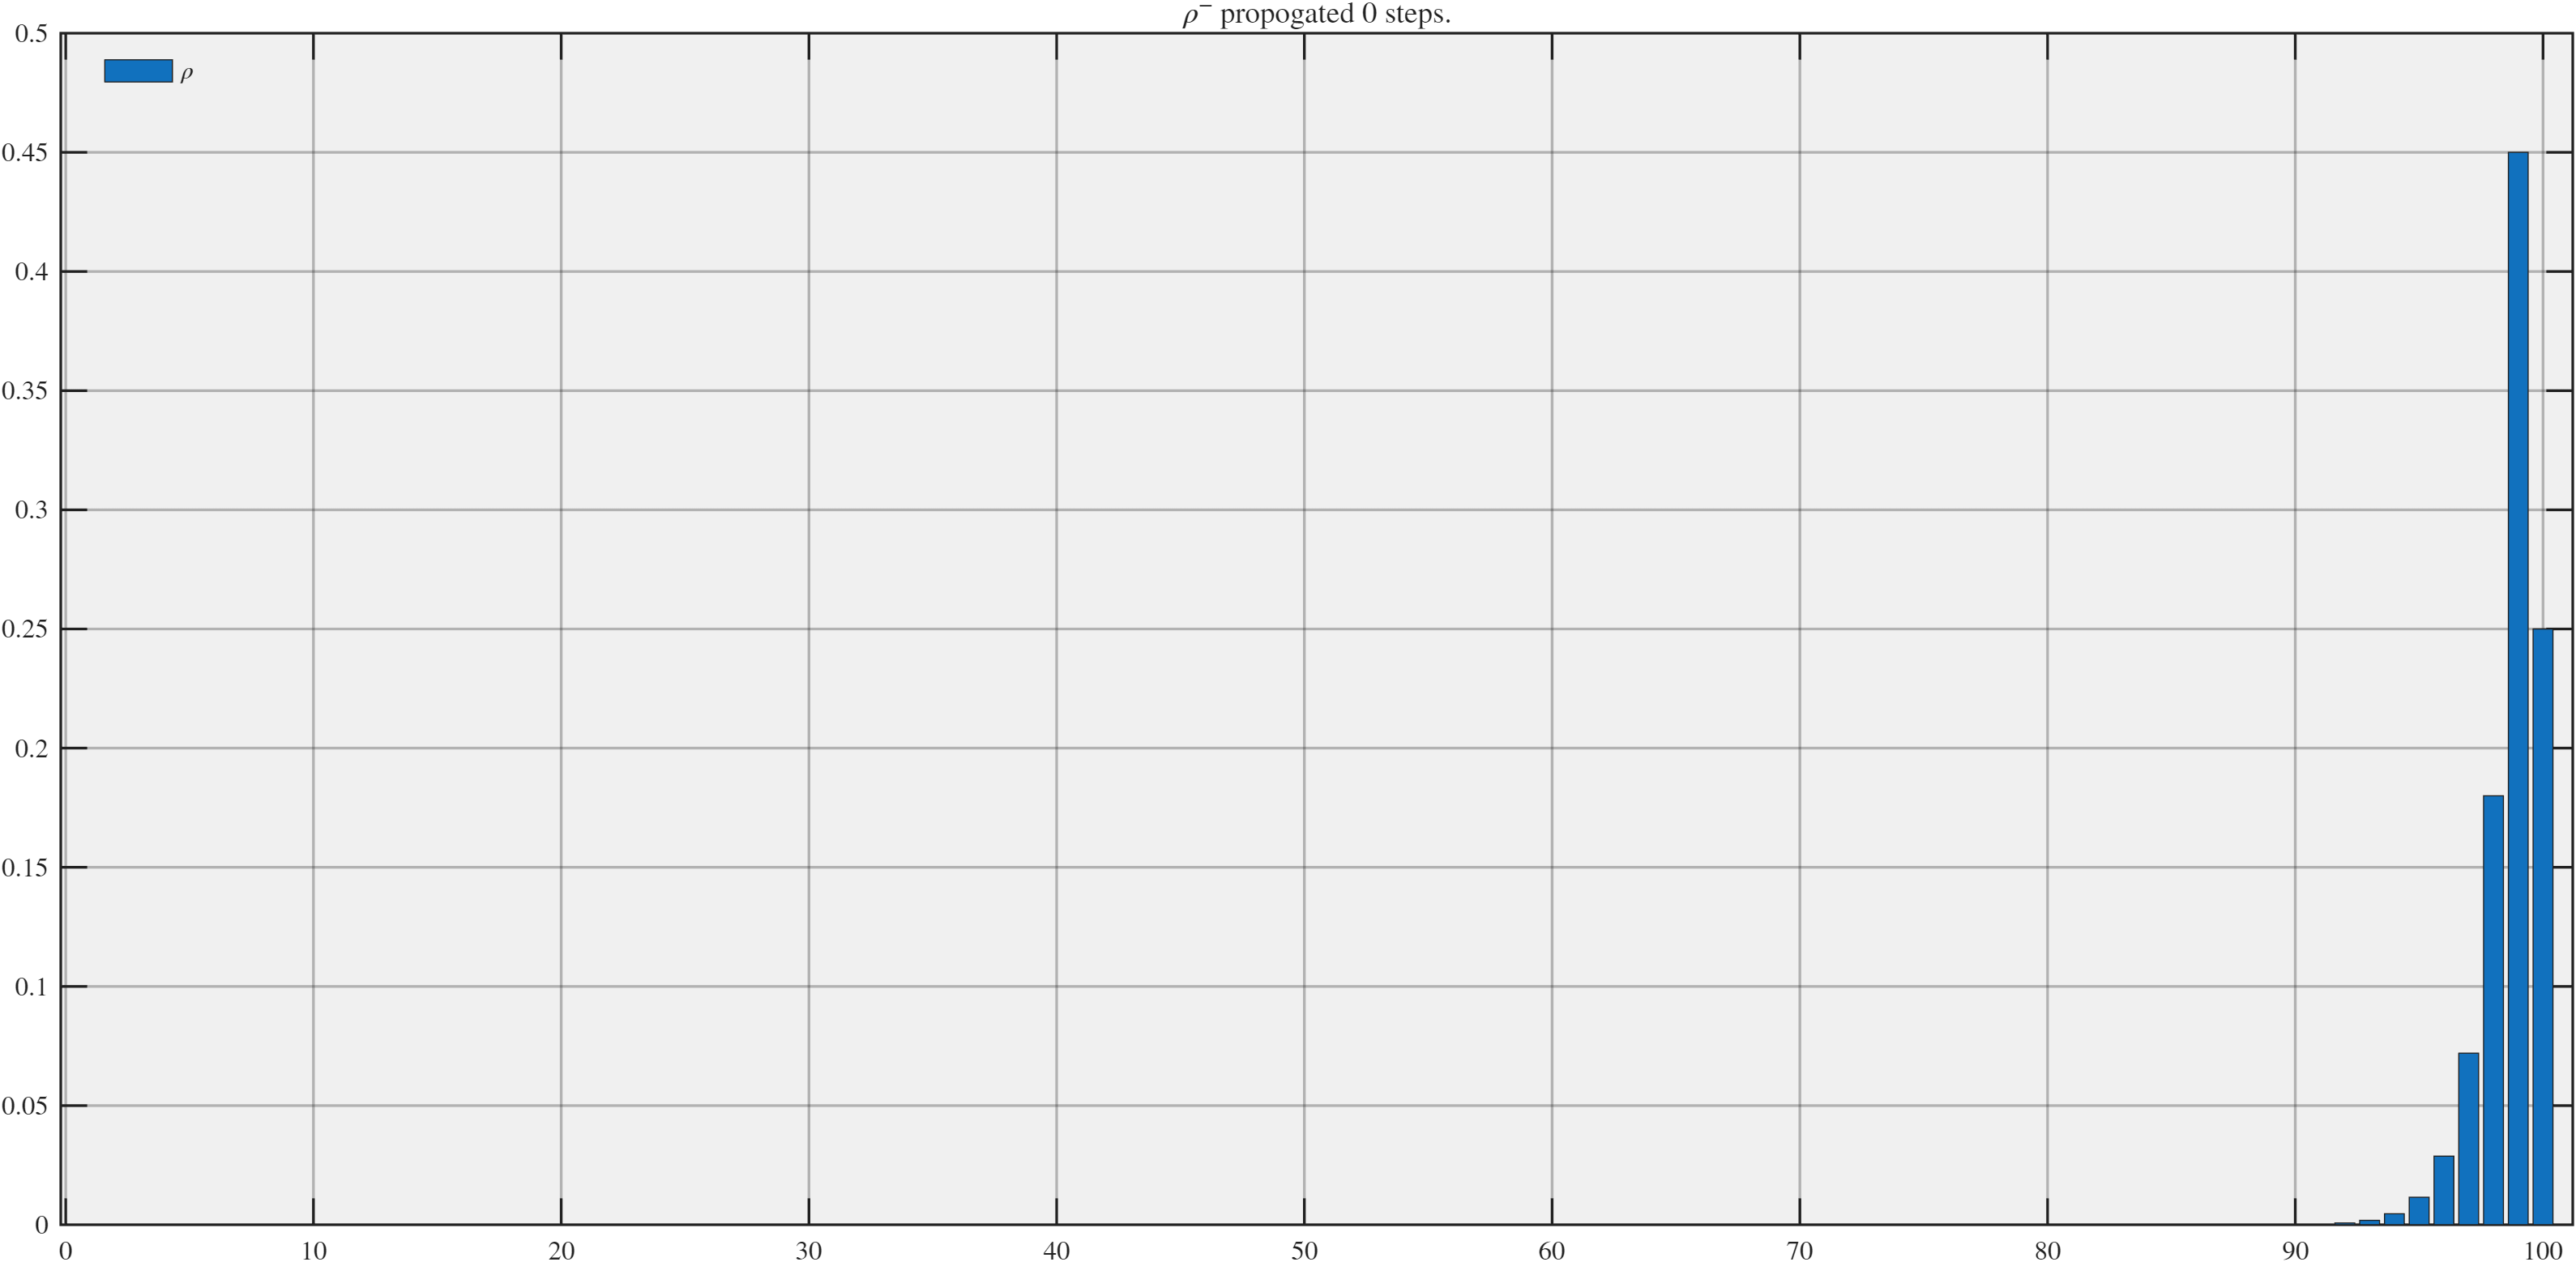
\includegraphics[width=\linewidth]{rho_propagated_000.png}
                \caption{$\rho^-_{\infty}$}
                \label{fig:rinf}
            \end{subfigure}

            \caption{Propagated distributions $\rho^-_k$ for selected $k$.}
        \end{figure}
        \item
            To implement a recursive Bayes filter to compute a posterior $\rho^+_k$, we can perform a Bayes update on our prior $\rho^-_k$.
            The full recursive Bayes filter for this problem is 
            \begin{align*}
                \rho^-_k &= T \rho^+_{k-1} \\ 
                \rho^+_k &\propto \mathcal{L}(z_k; \zeta_k) \rho^-_k \\
                \mathcal{L}(z_k; \zeta_k) &= P(z_k=i \mid \zeta_k = j) = \mathcal{U}_{i\mid j}[a(r),b(r)]
	        \end{align*} 

            The results at the selected timesteps are summarized in figure \ref{fig:grid_filter_snapshots} and table \ref{tab:grid_mmse_map}.
            Compared to the truth $\zeta$ values we see that the exact Bayes filter MMSE and MAP estimates are both very close to the ground truth values. 
	            \begin{figure}[H]
	                \centering
	                \begin{subfigure}[t]{0.32\textwidth}
	                    \centering
	                    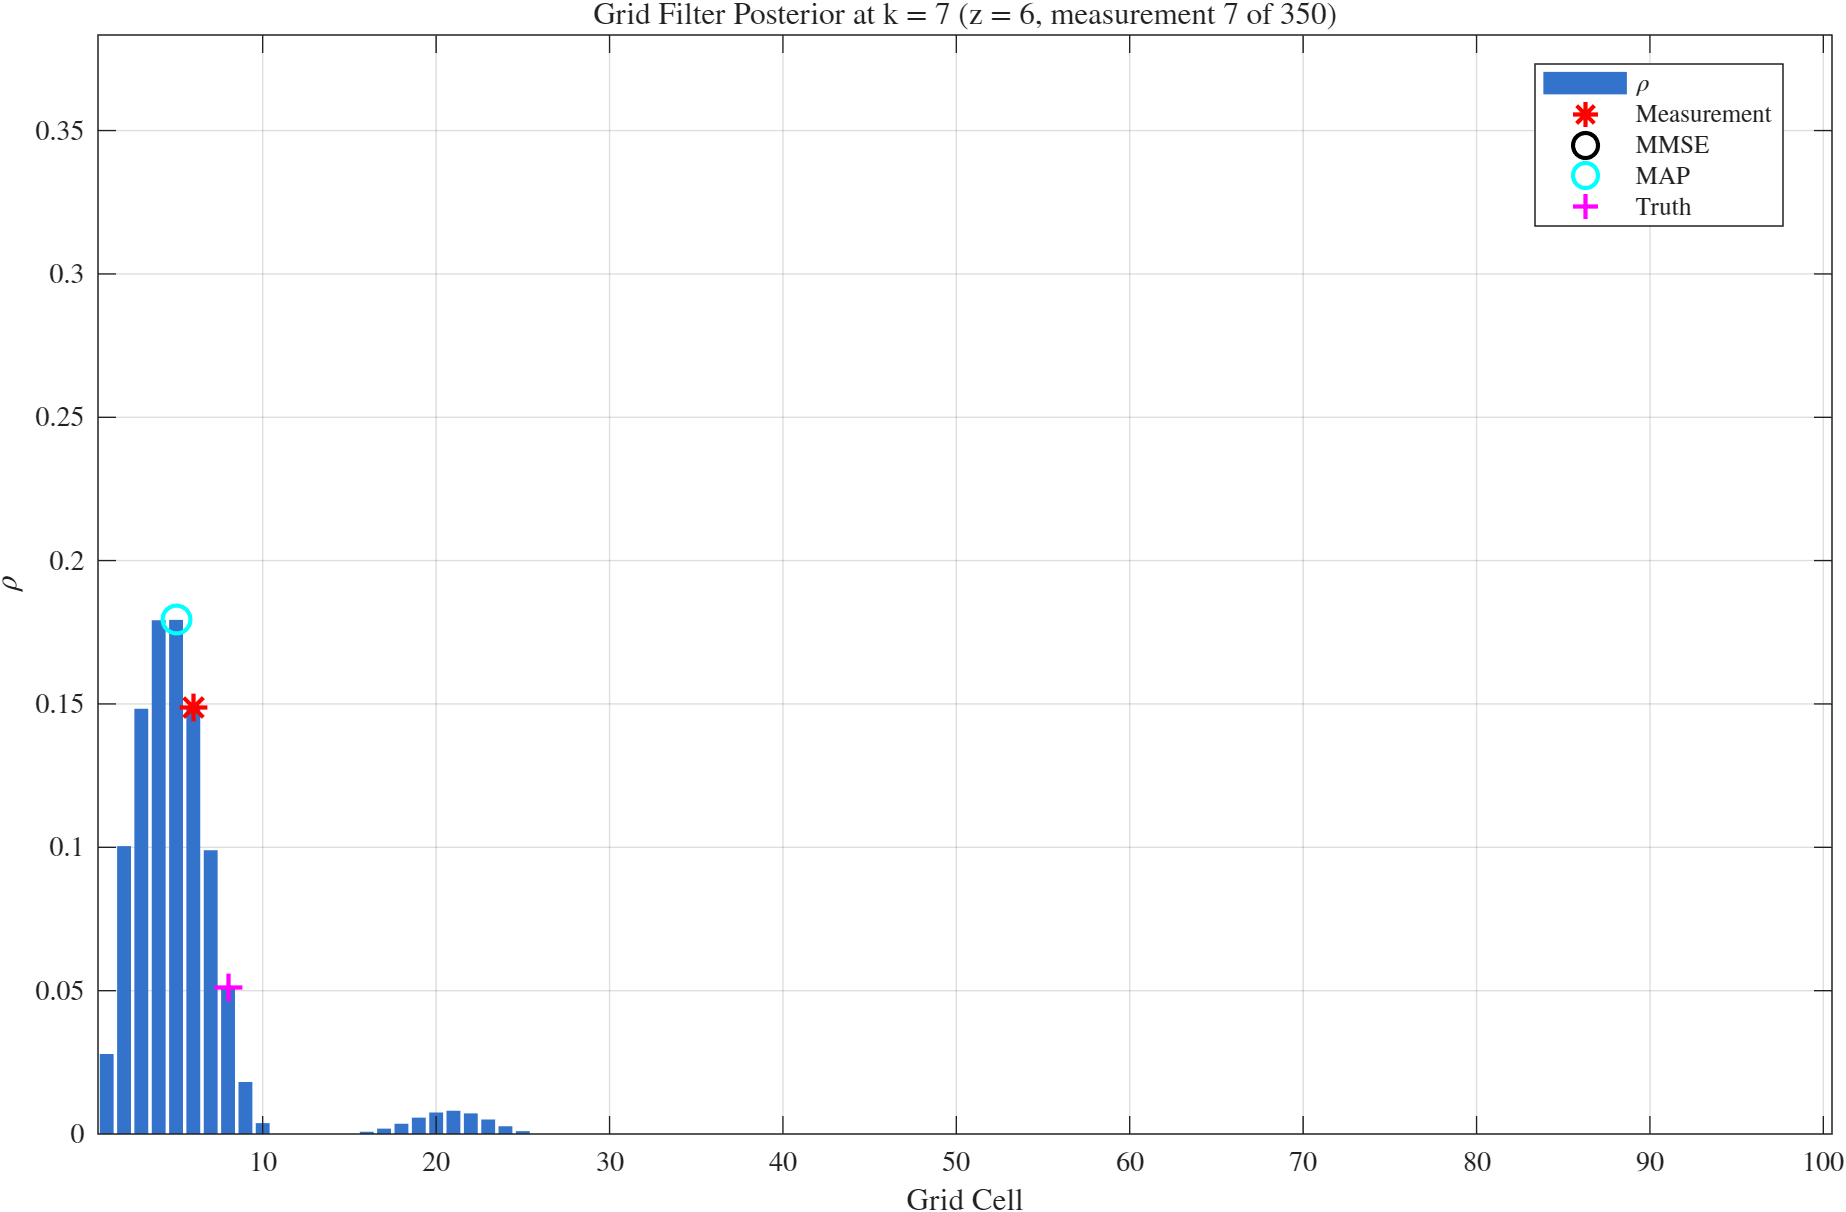
\includegraphics[width=\linewidth]{grid_filter_frame_007.png}
	                    \caption{$k=7$}
	                    \label{fig:grid007}
	                \end{subfigure}
	                \hfill
	                \begin{subfigure}[t]{0.32\textwidth}
	                    \centering
	                    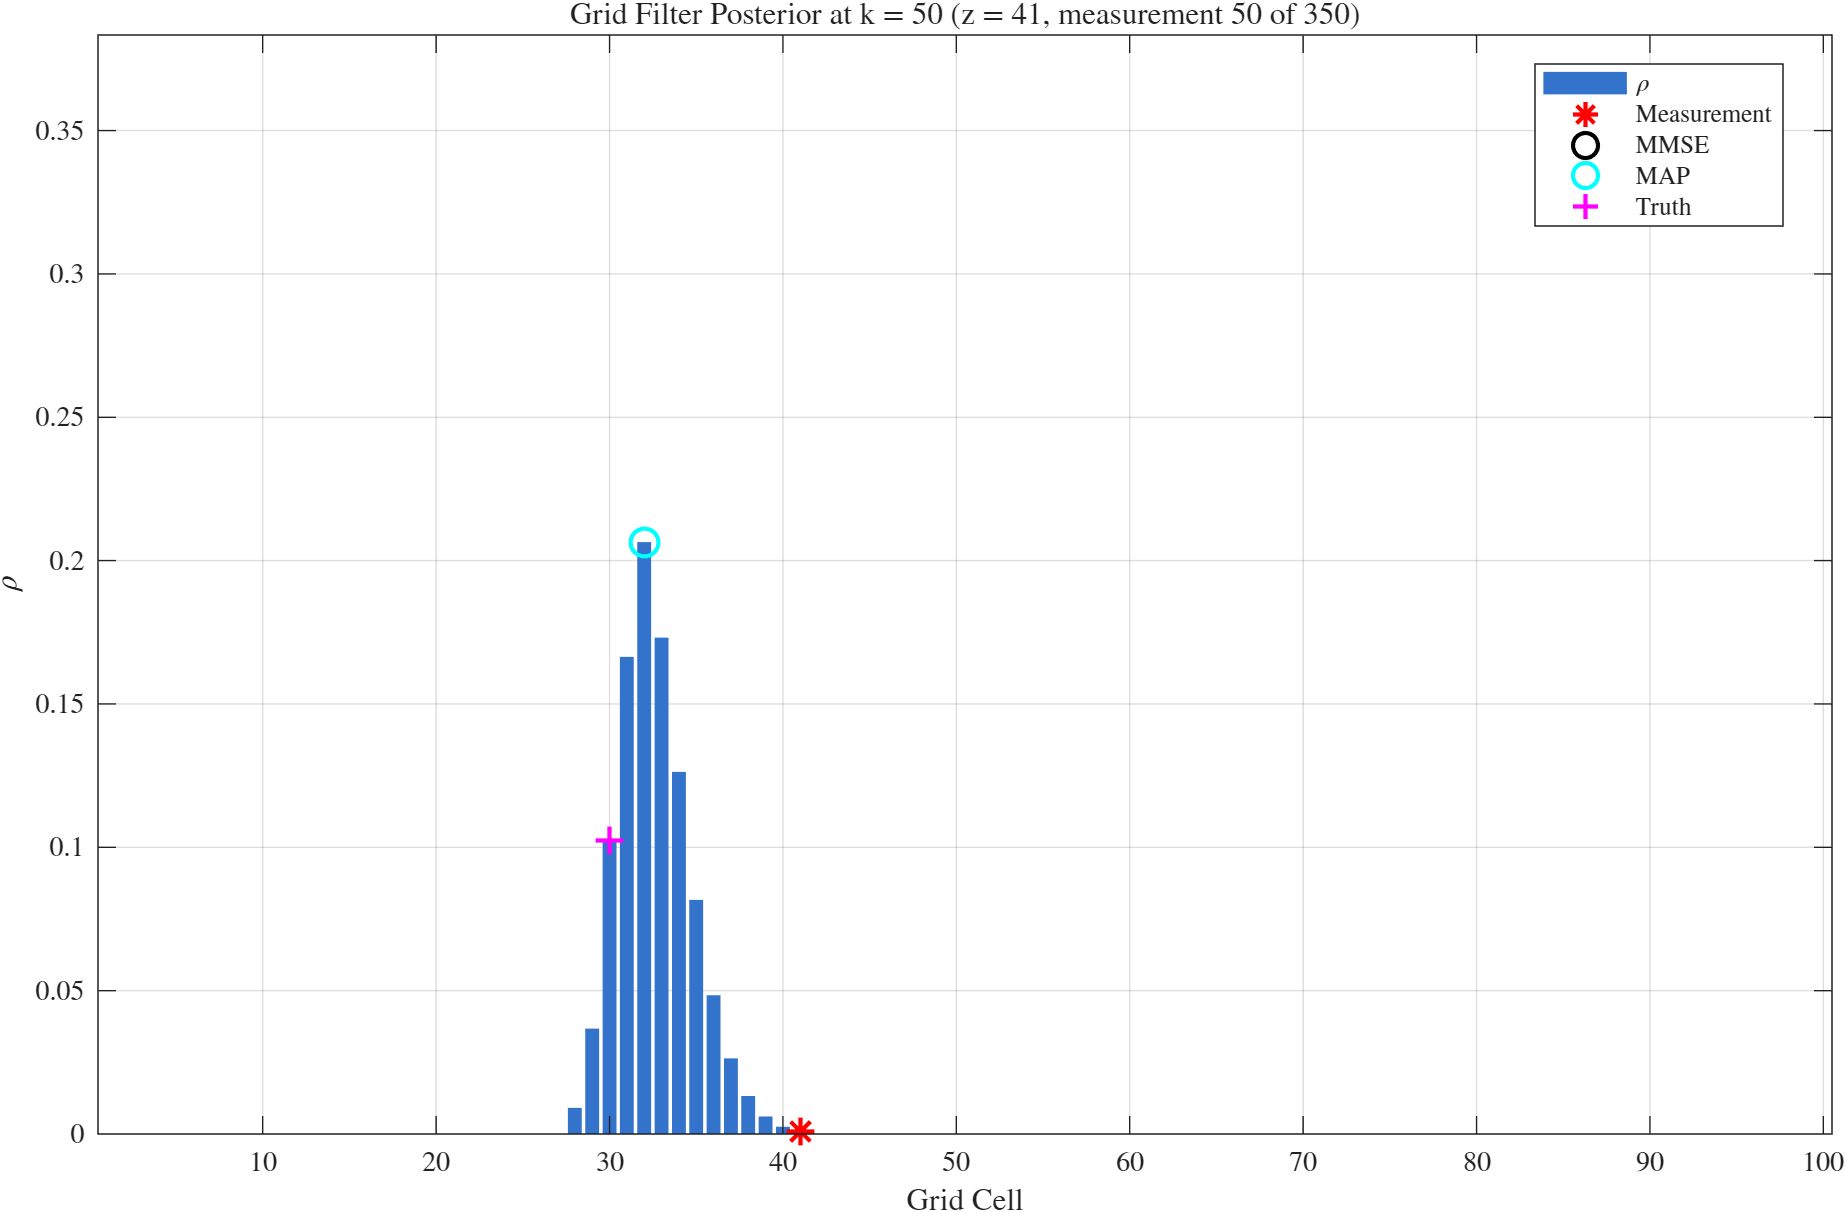
\includegraphics[width=\linewidth]{grid_filter_frame_050.png}
	                    \caption{$k=50$}
	                    \label{fig:grid050}
	                \end{subfigure}
	                \hfill
	                \begin{subfigure}[t]{0.32\textwidth}
	                    \centering
	                    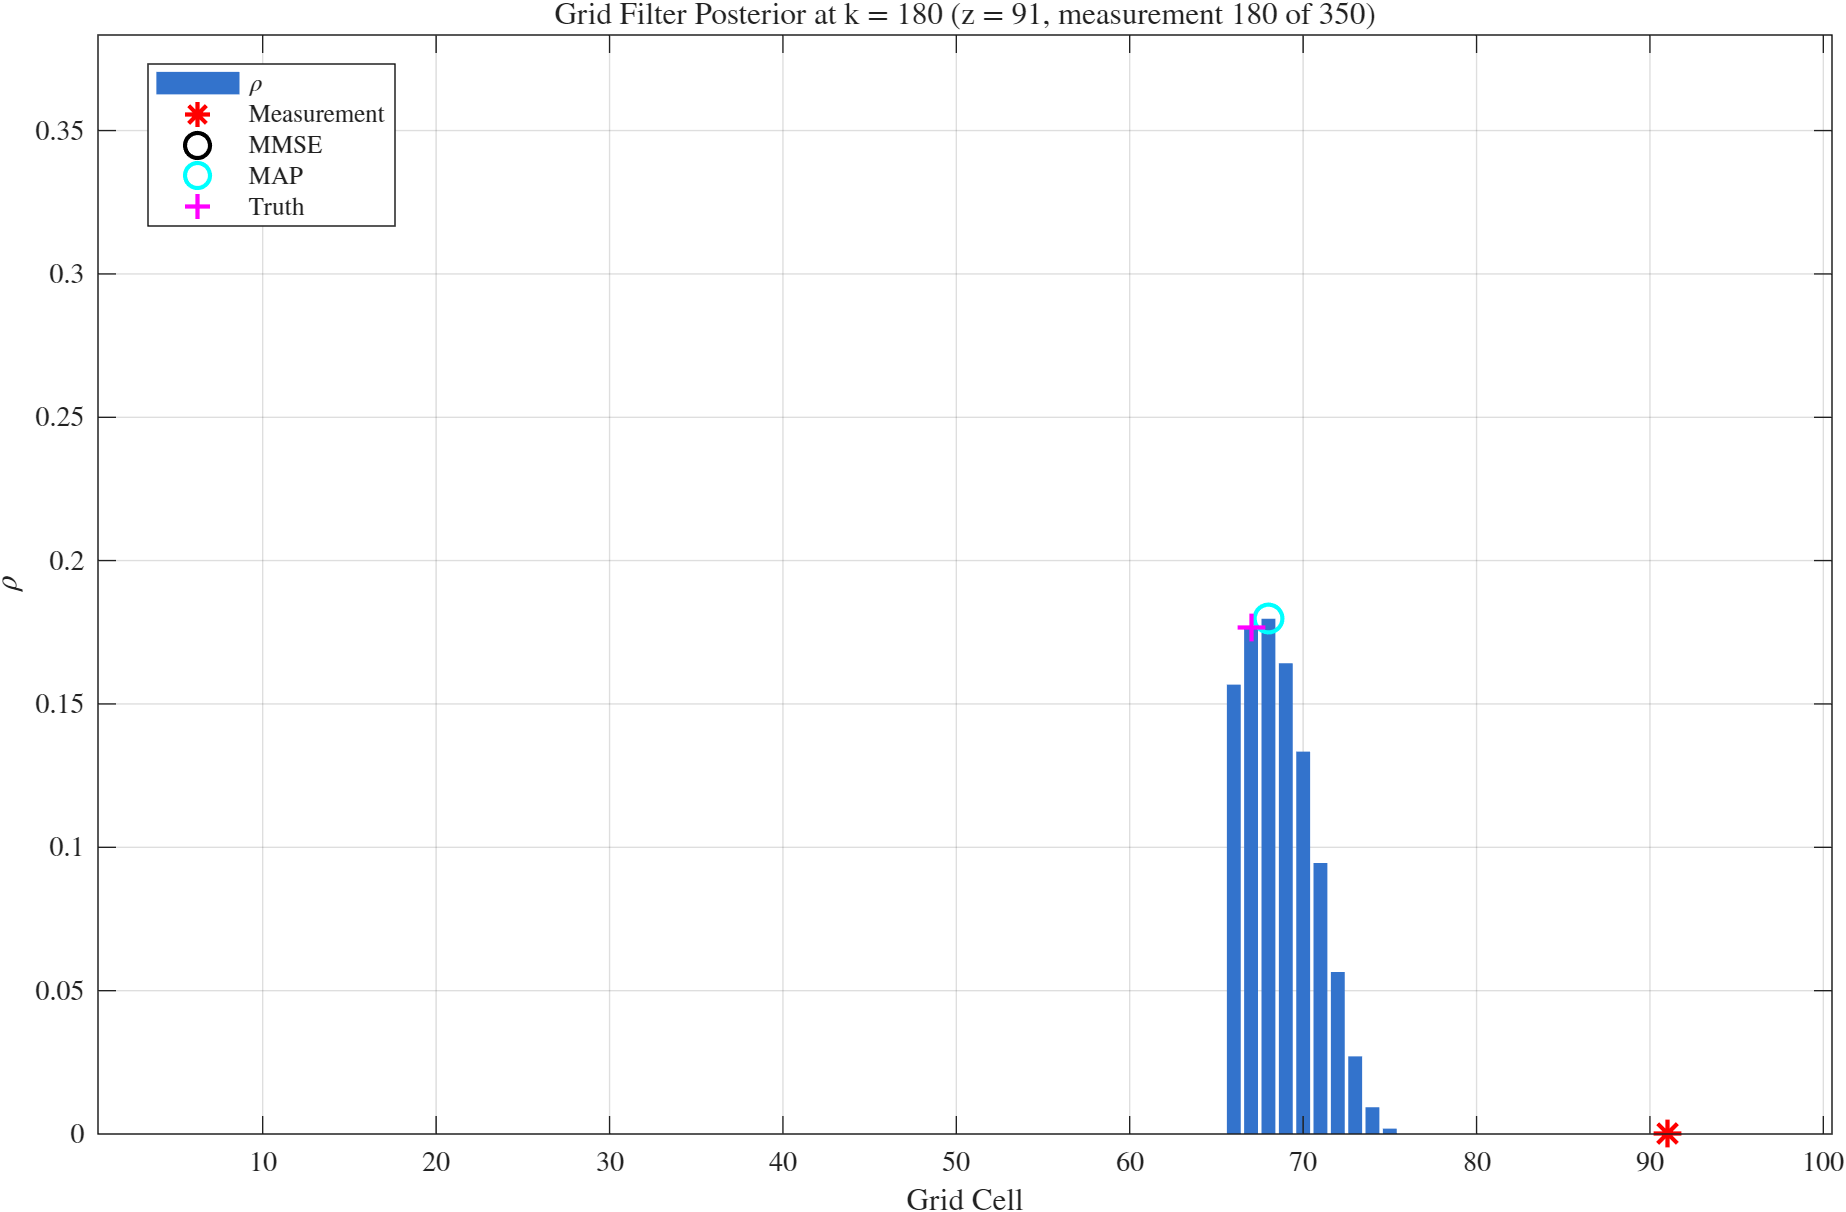
\includegraphics[width=\linewidth]{grid_filter_frame_180.png}
	                    \caption{$k=180$}
	                    \label{fig:grid180}
	                \end{subfigure}

	                \vspace{0.6em}

	                \begin{subfigure}[t]{0.32\textwidth}
	                    \centering
	                    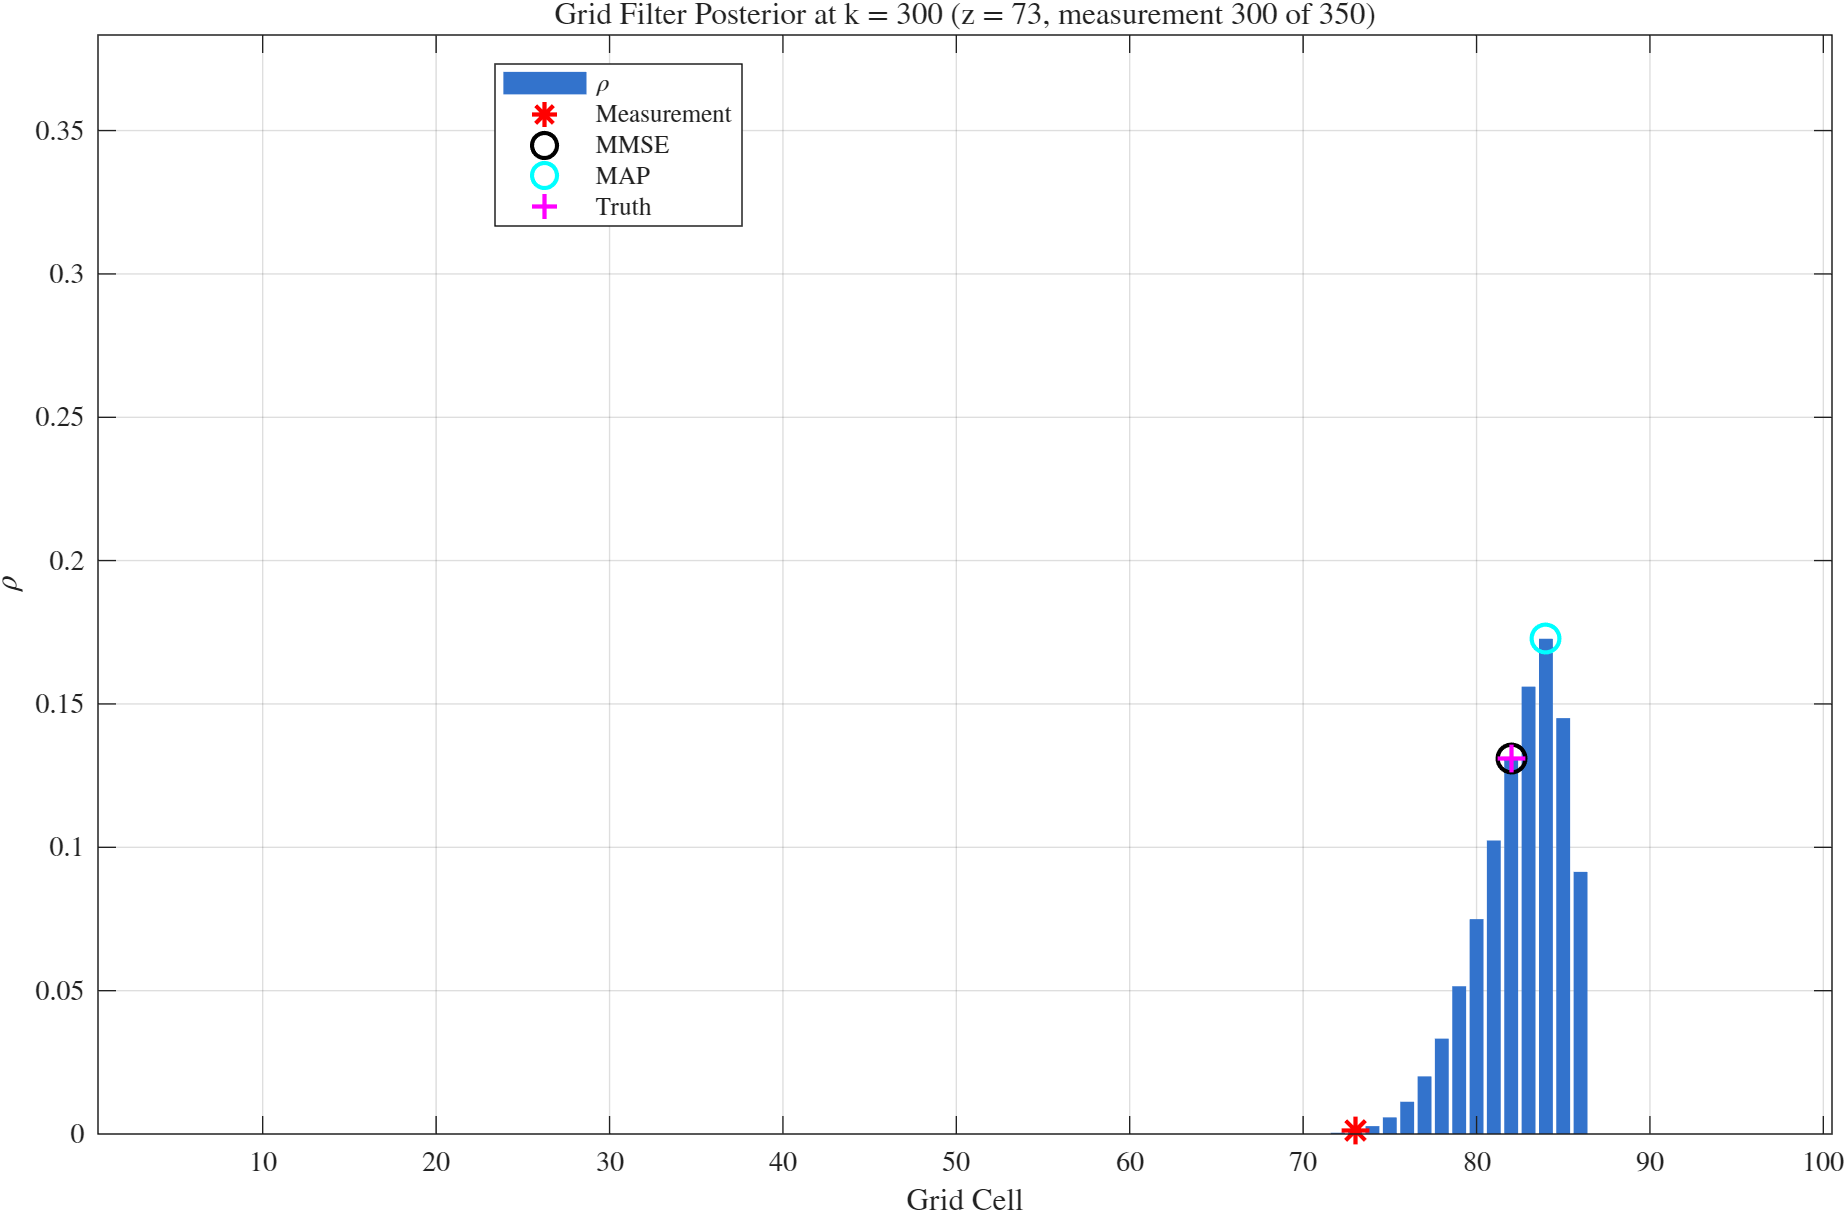
\includegraphics[width=\linewidth]{grid_filter_frame_300.png}
	                    \caption{$k=300$}
	                    \label{fig:grid300}
	                \end{subfigure}
	                \hfill
	                \begin{subfigure}[t]{0.32\textwidth}
	                    \centering
	                    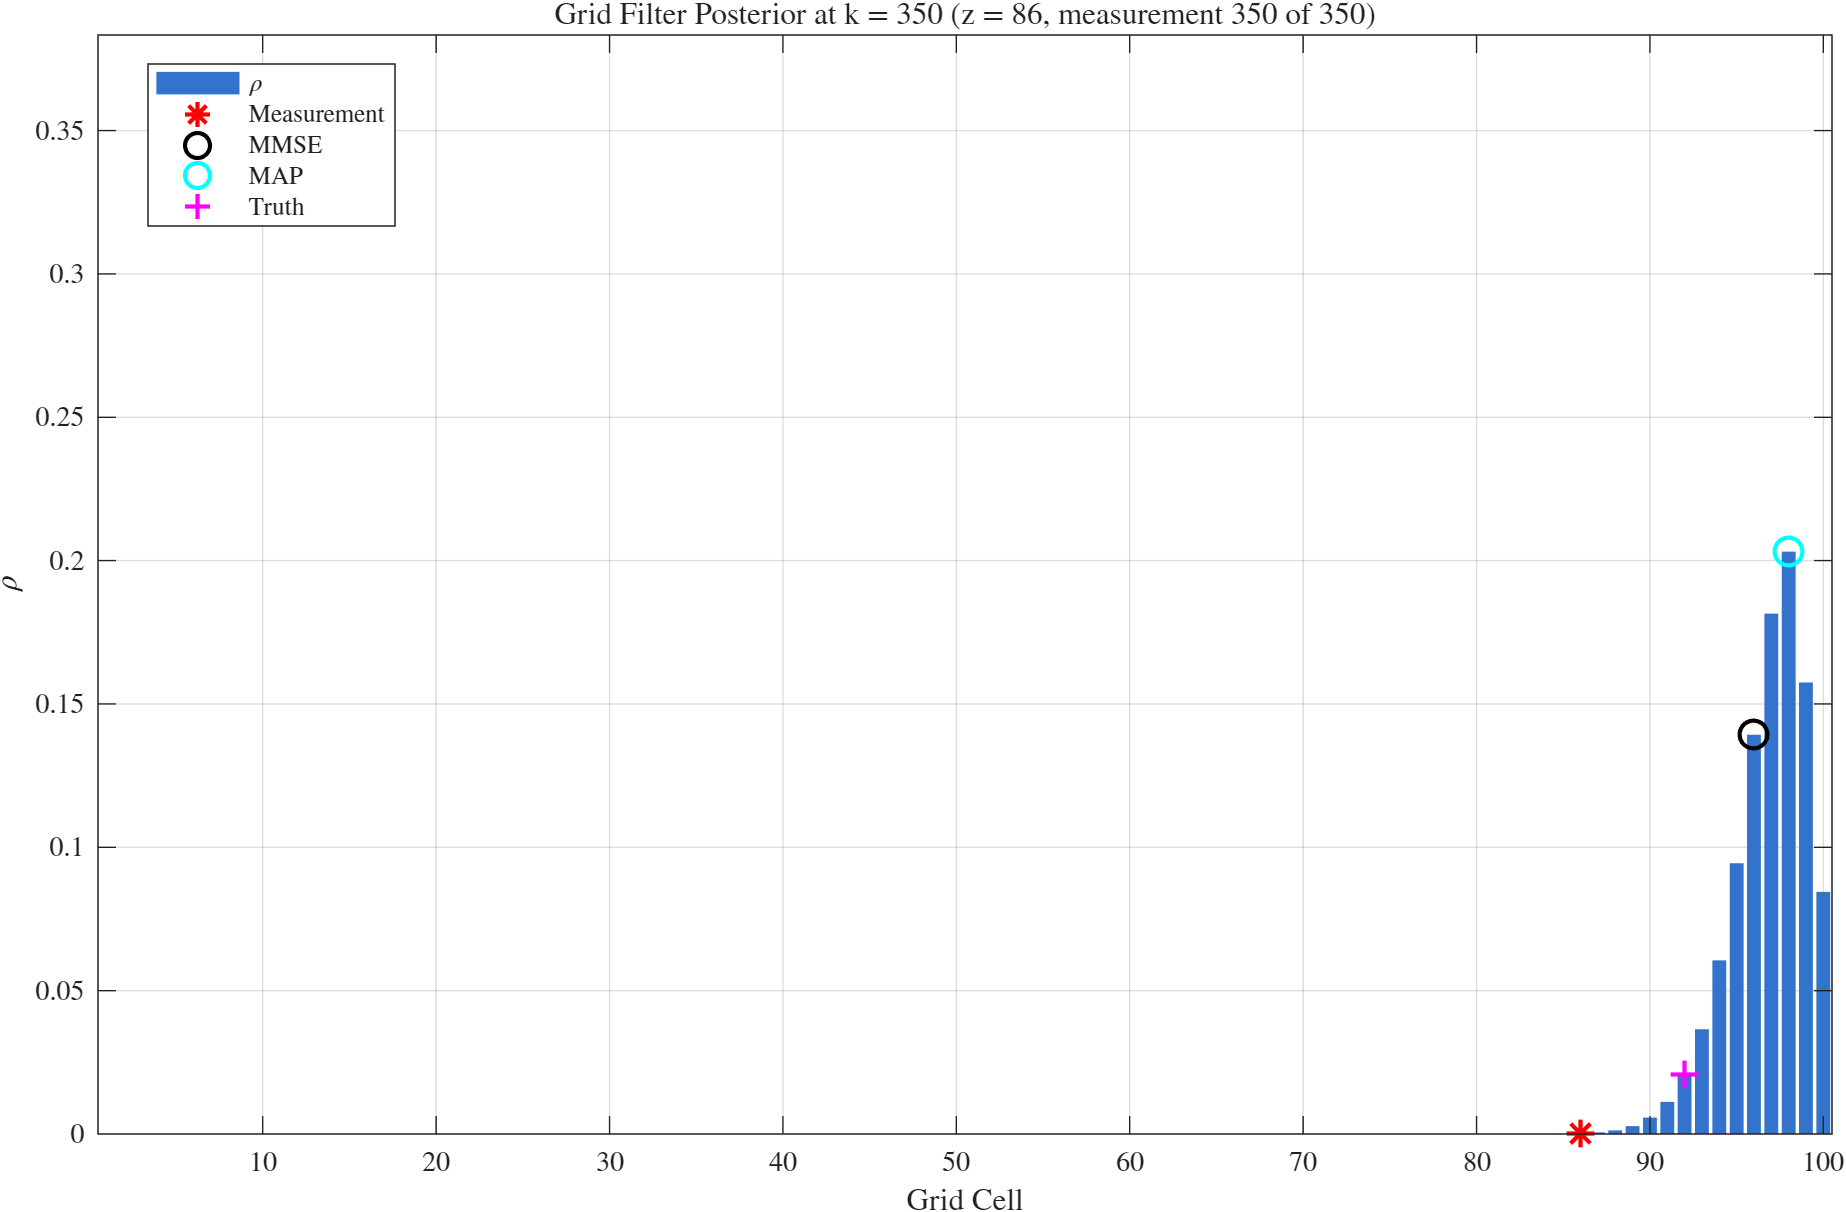
\includegraphics[width=\linewidth]{grid_filter_frame_350.png}
	                    \caption{$k=350$}
	                    \label{fig:grid350}
	                \end{subfigure}

	                \caption{Grid-filter posterior snapshots at selected timesteps.}
	                \label{fig:grid_filter_snapshots}
		            \end{figure}
	            \begin{table}[H]
	                \centering
	                \caption{Grid-filter MMSE and MAP estimates at selected timesteps}
	                \label{tab:grid_mmse_map}
	                \begin{tabular}{cccc}
	                    \toprule
	                    Timestep $k$ & MMSE Cell Index & MAP Cell Index & Ground Truth\\
	                    \midrule
	                    7   & 5 & 4 & 7\\
	                    50  & 32 & 31 & 30\\
	                    180 & 67 & 67 & 66\\
	                    300 & 82 & 84 & 82\\
	                    350 & 96 & 97 & 93\\
	                    \bottomrule
	                \end{tabular}
	            \end{table}
	        \item
                The bootstrap particle filter sets the proposal distribution as the transition pdf $P(\zeta_{k+1} = i \mid \zeta_k+j)$ and resamples after each measurment weight update.
                The choice of importance distribution allows the weight update to simplify to observation likelihood which makes implementation very easy. 
                Figure \ref{fig:pf_filter_snapshots} shows the approximate posterior at the specified time steps using the weighted sum of particles to approximate the distribution shape.
                The MMSE and MAP estimates are summarized in table \ref{tab:PF_mmse_map}. The estimates are very similar to the exact Bayes grid filter indicating that the bootstrap PF does a very good job at approximating the exact distribution. 
                The MMSE and MAP estimates across each timestep for the grid and PF are summarized in figure \ref{fig:tot}.
                	            \begin{figure}[H]
	                \centering
	                \begin{subfigure}[t]{0.32\textwidth}
	                    \centering
	                    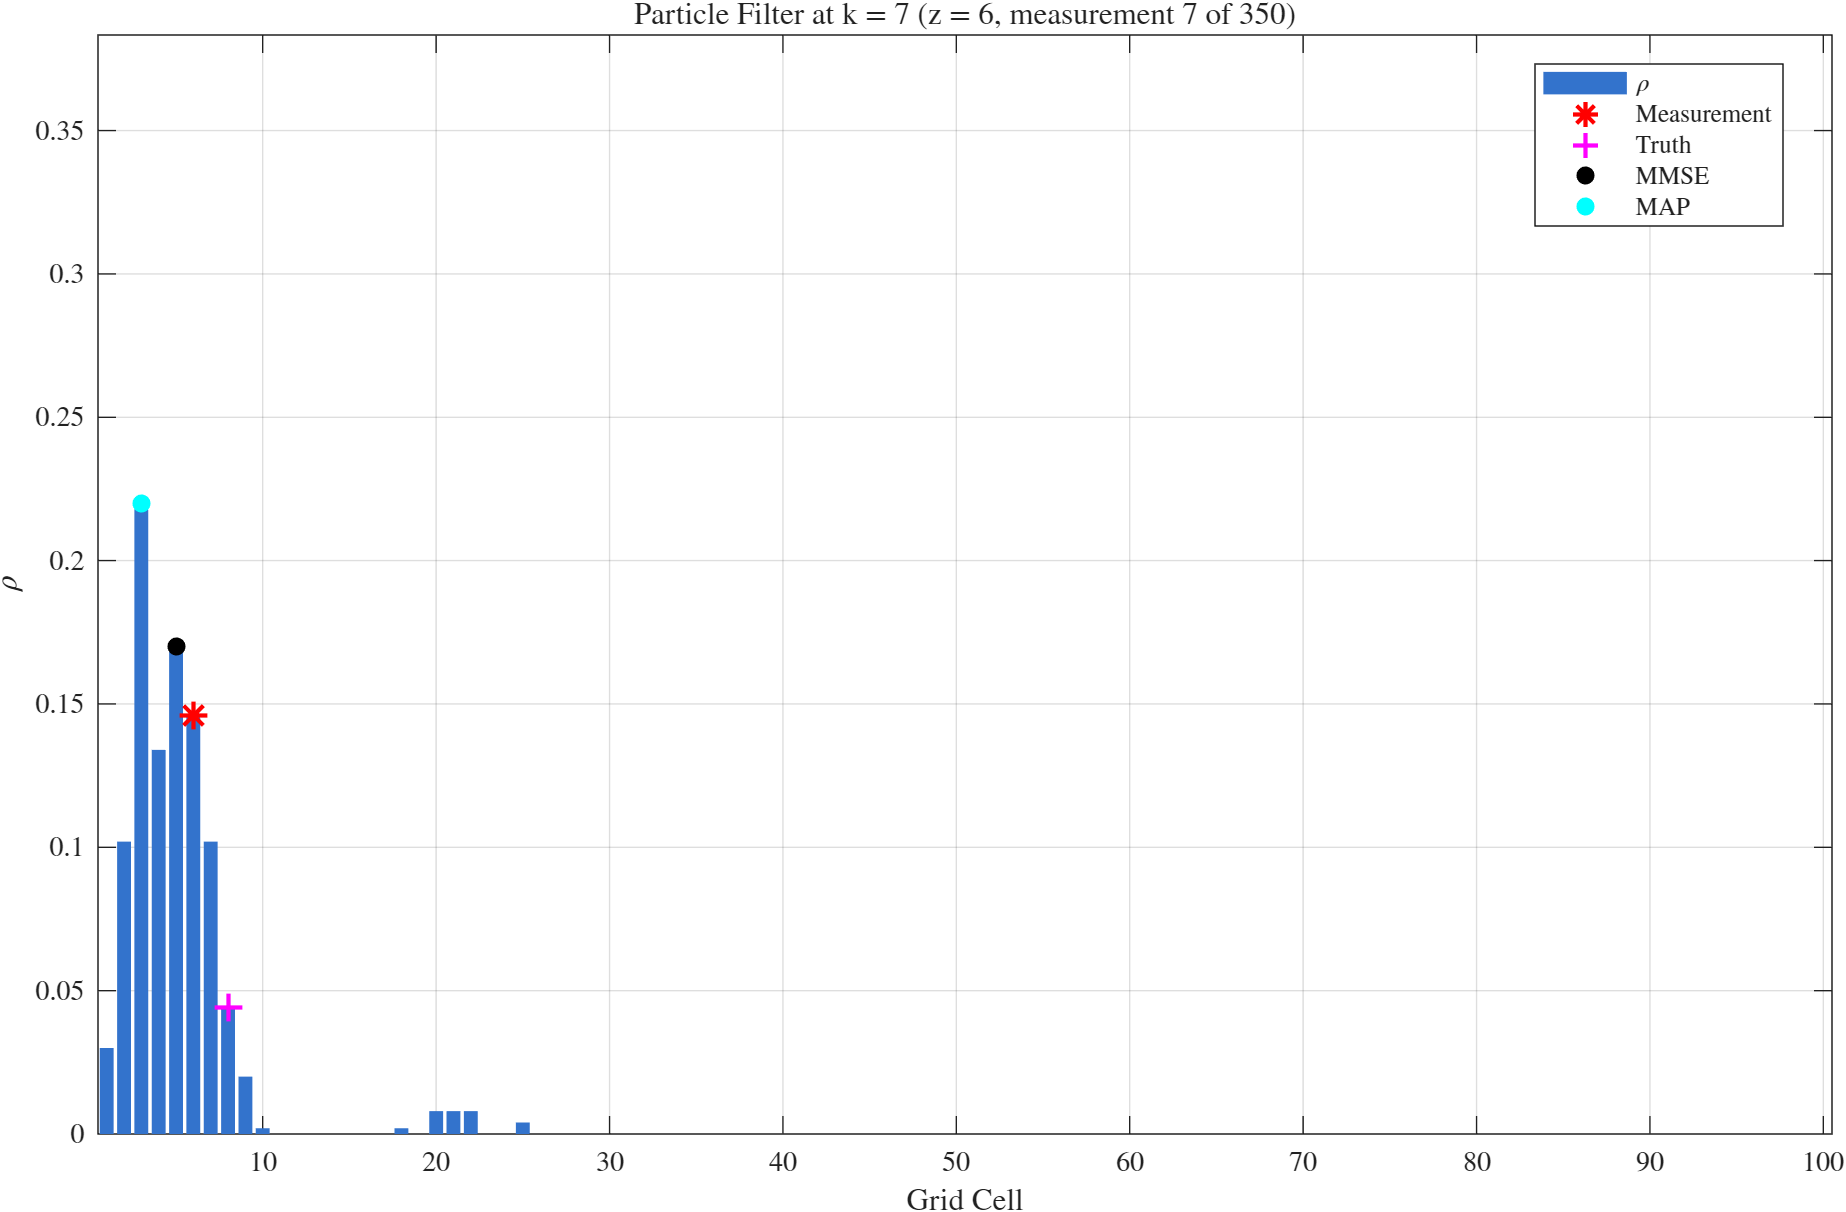
\includegraphics[width=\linewidth]{pf_filter_frame_007.png}
	                    \caption{$k=7$}
	                    \label{fig:pf007}
	                \end{subfigure}
	                \hfill
	                \begin{subfigure}[t]{0.32\textwidth}
	                    \centering
	                    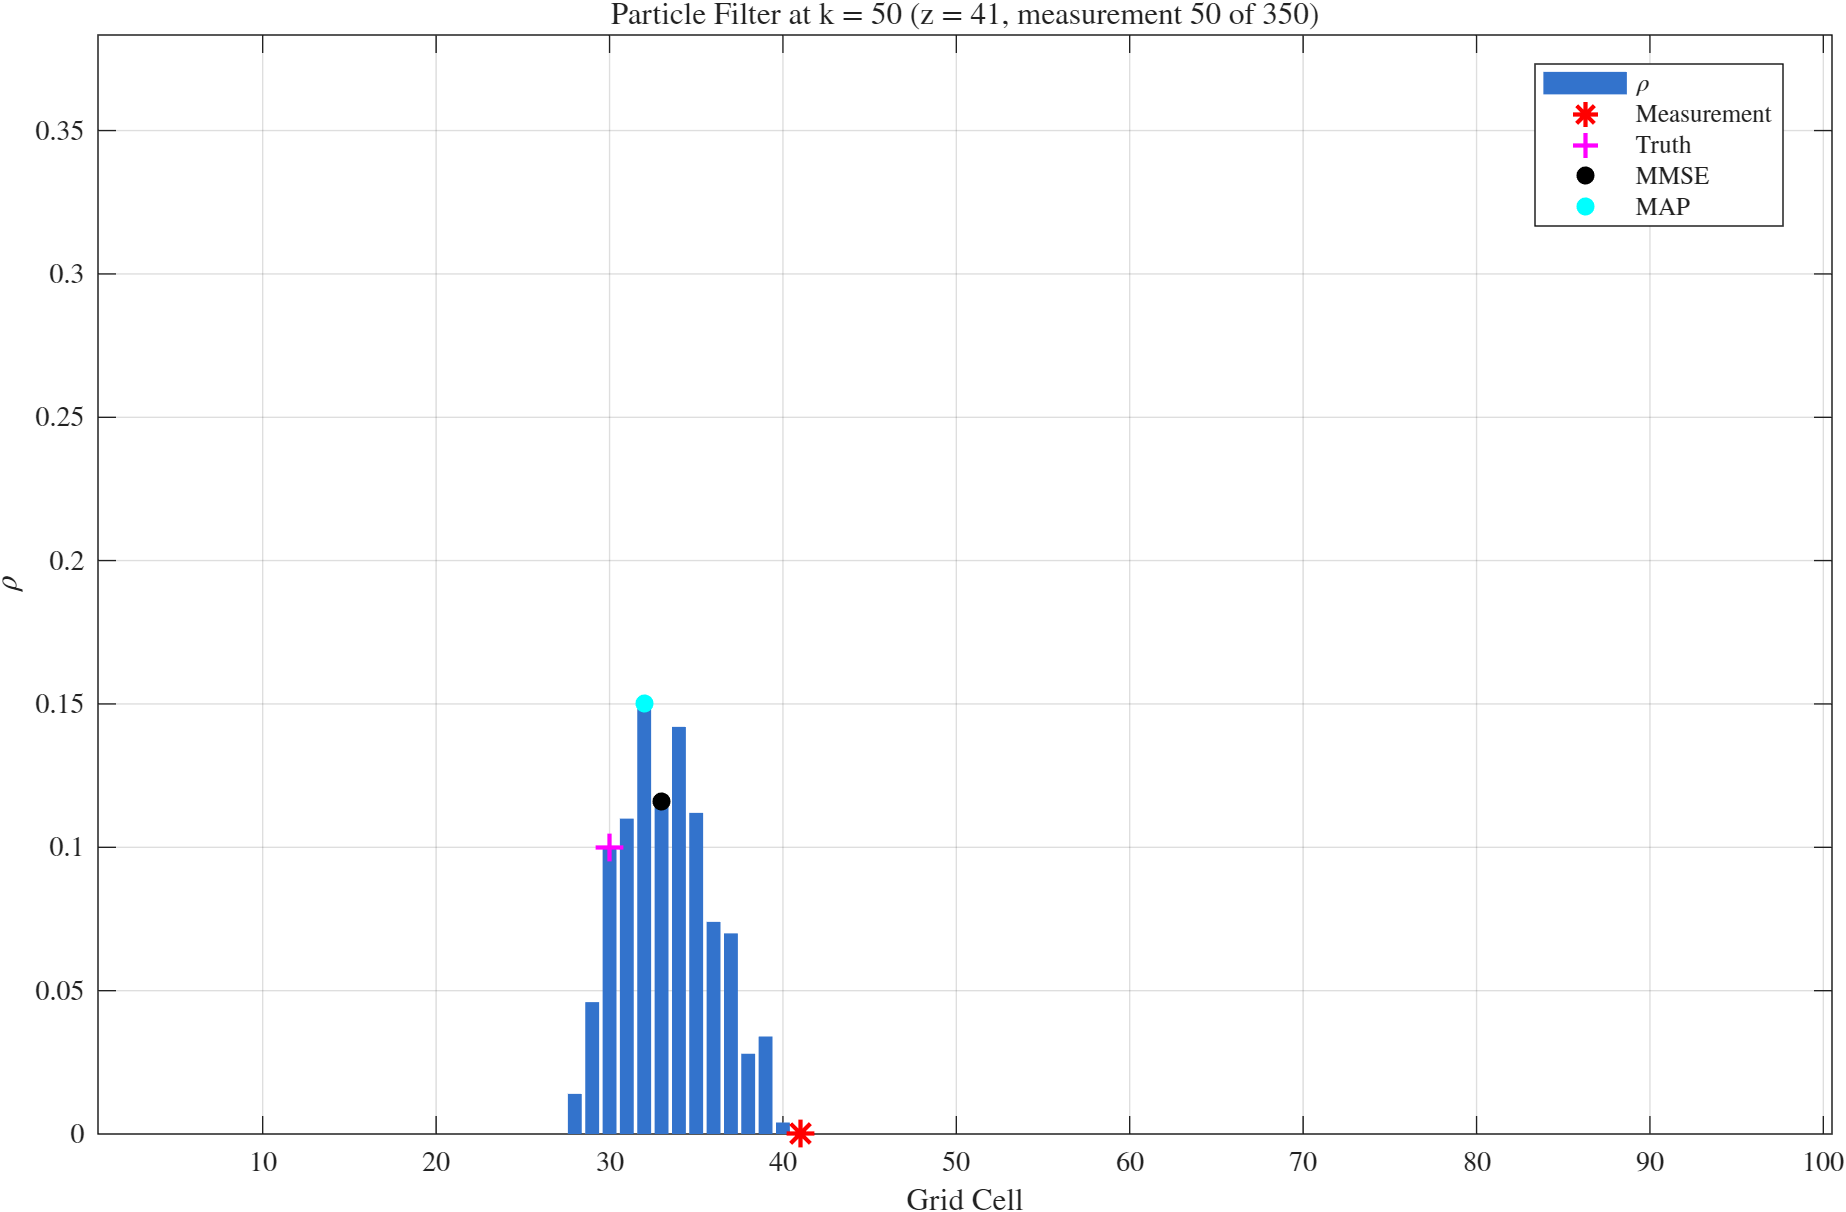
\includegraphics[width=\linewidth]{pf_filter_frame_050.png}
	                    \caption{$k=50$}
	                    \label{fig:pf050}
	                \end{subfigure}
	                \hfill
	                \begin{subfigure}[t]{0.32\textwidth}
	                    \centering
	                    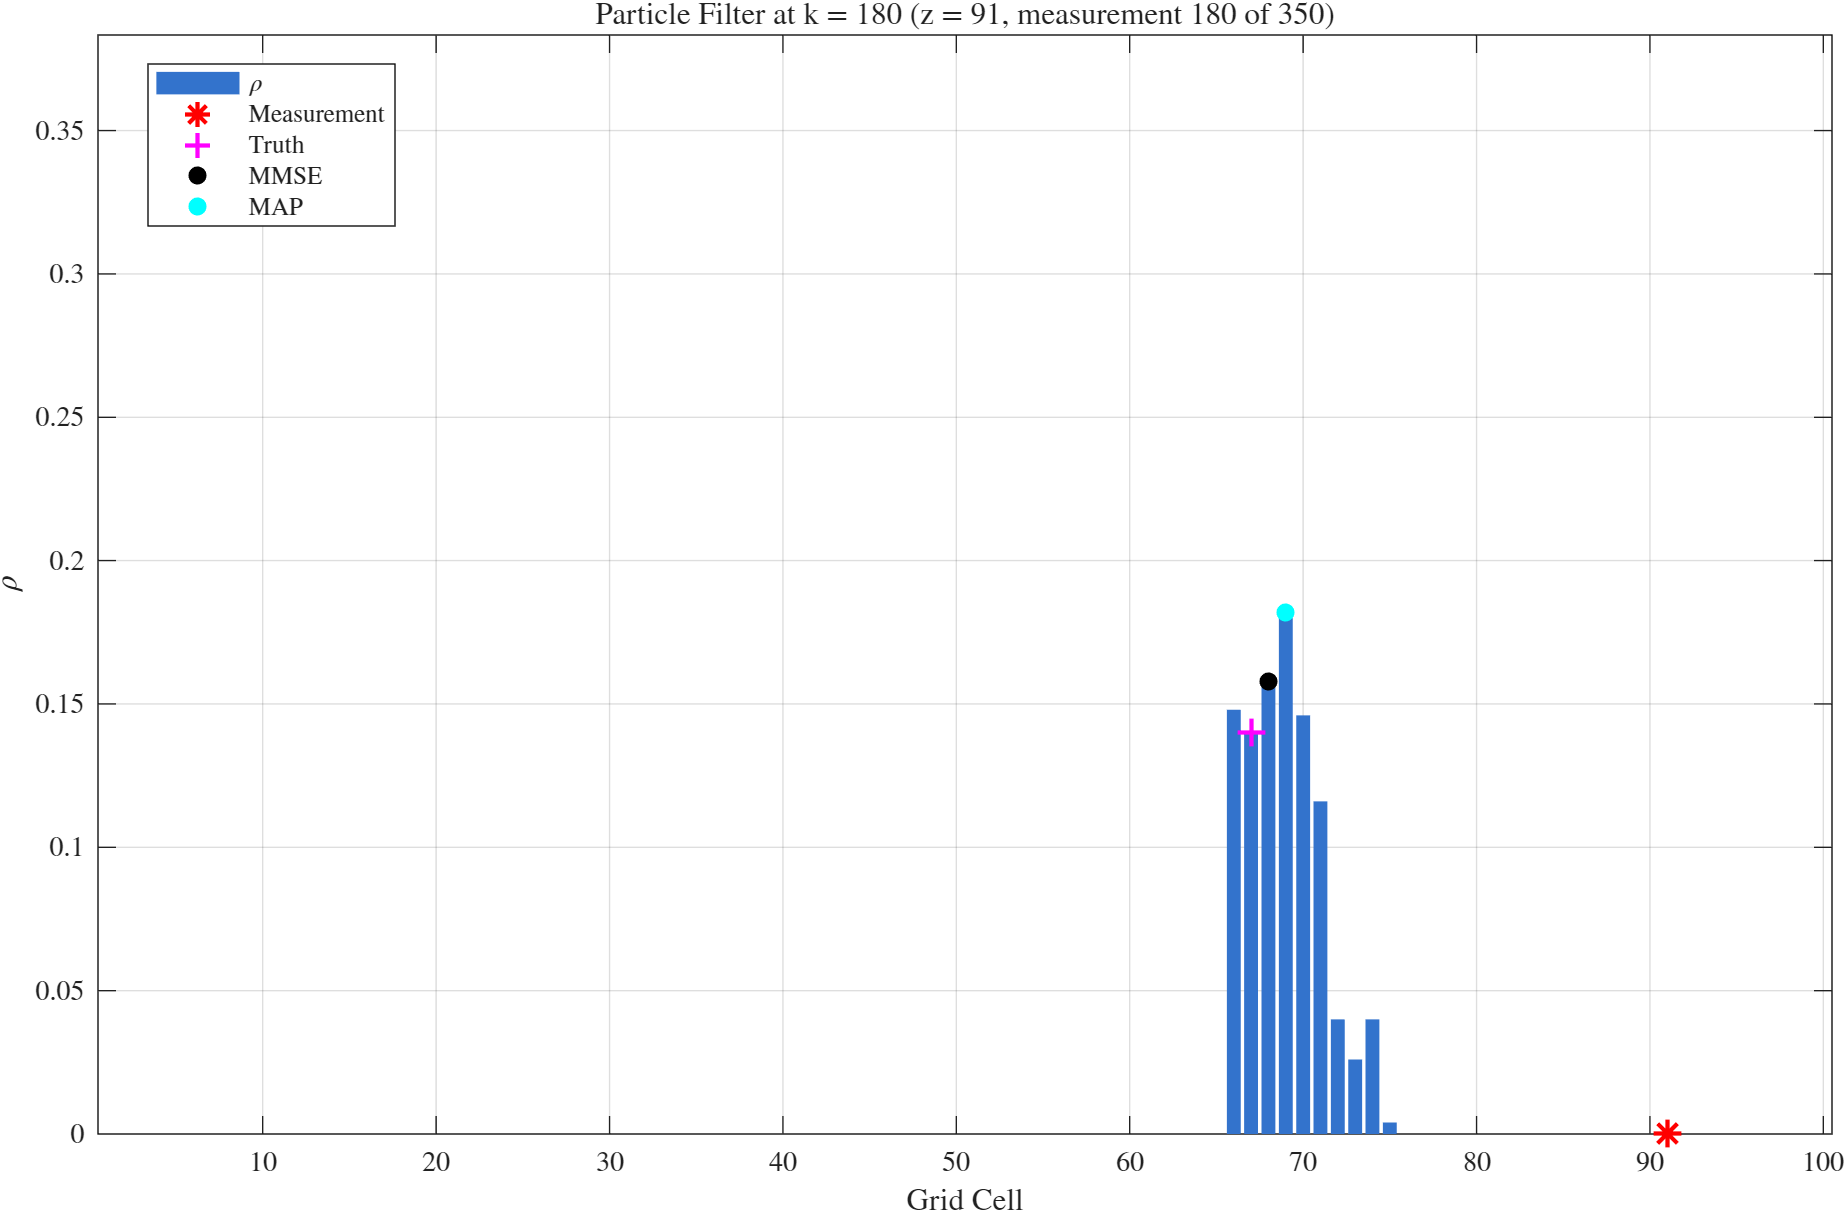
\includegraphics[width=\linewidth]{pf_filter_frame_180.png}
	                    \caption{$k=180$}
	                    \label{fig:pf180}
	                \end{subfigure}

	                \vspace{0.6em}

	                \begin{subfigure}[t]{0.32\textwidth}
	                    \centering
	                    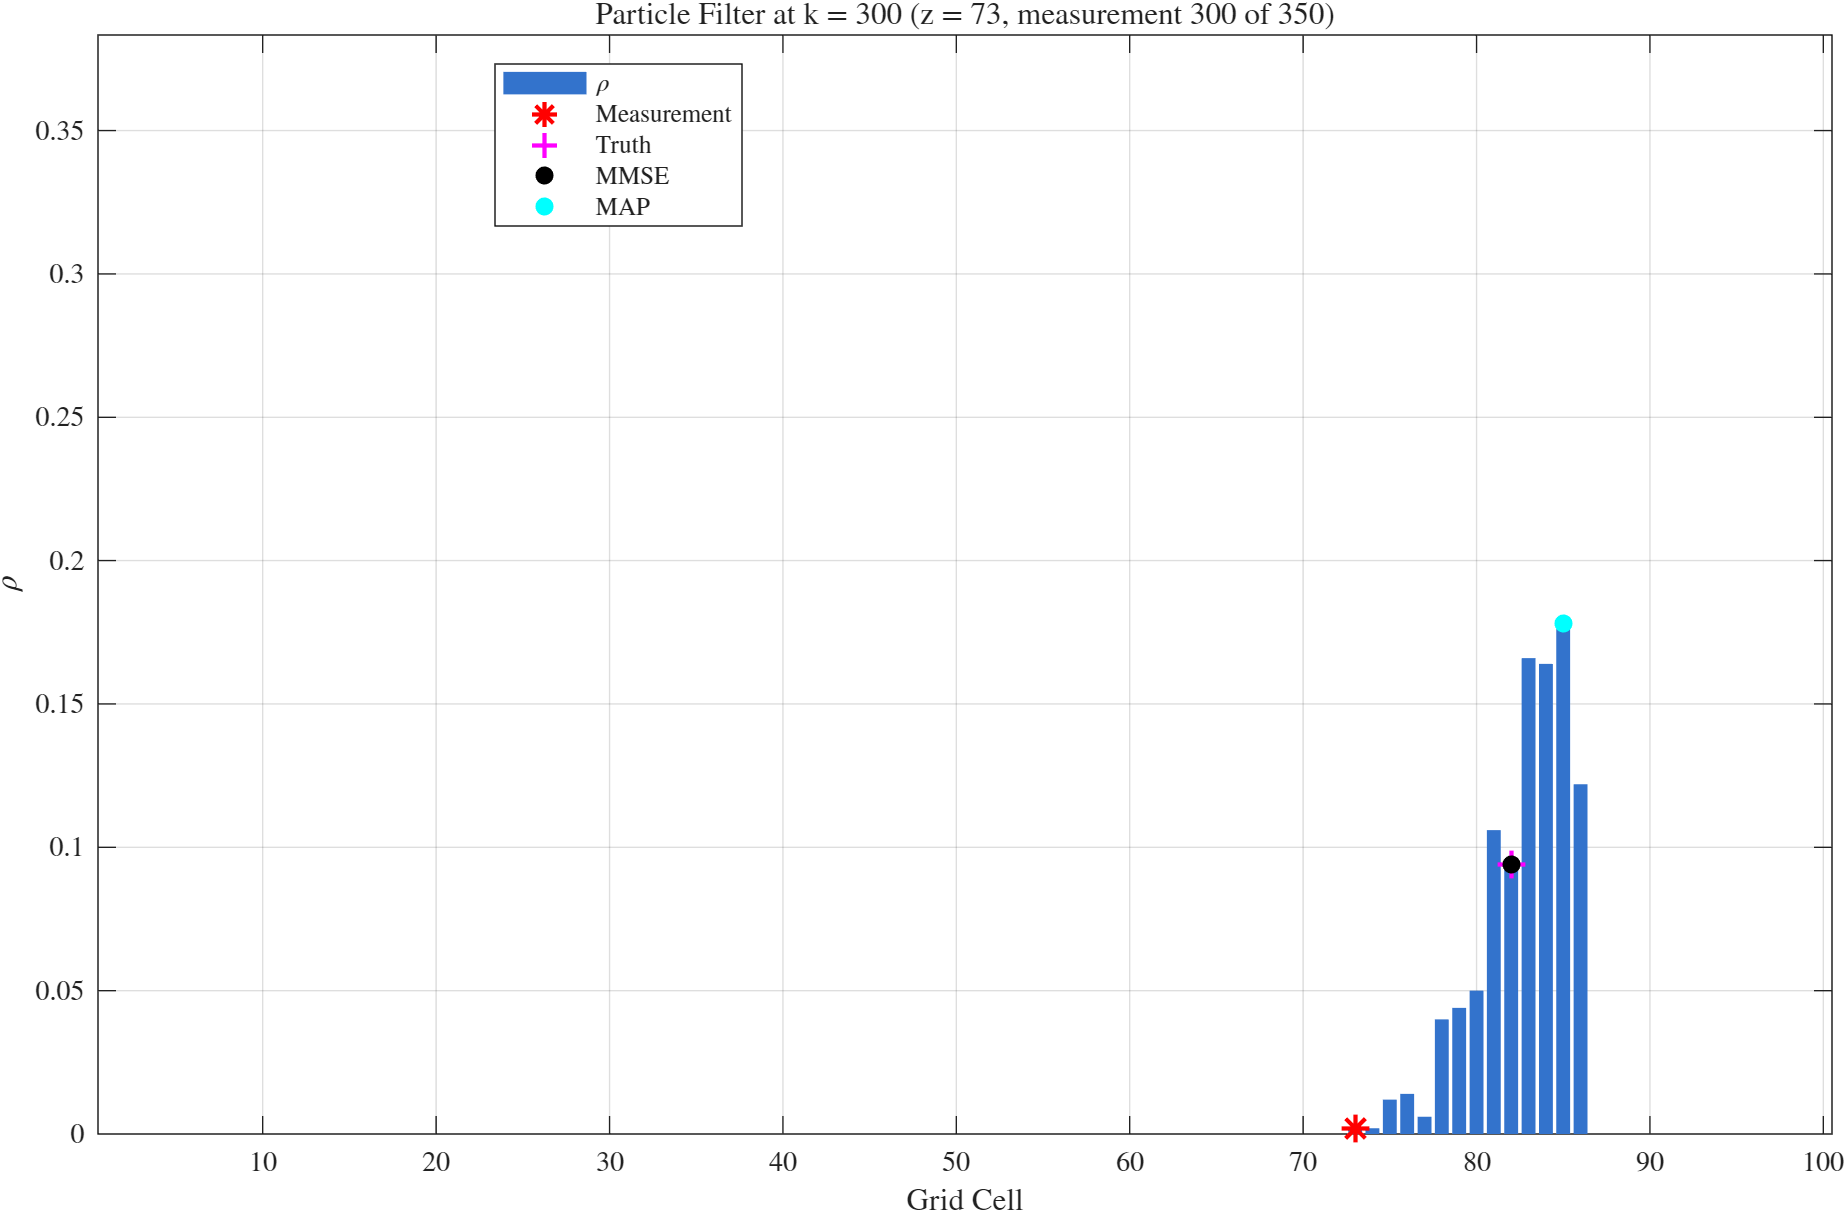
\includegraphics[width=\linewidth]{pf_filter_frame_300.png}
	                    \caption{$k=300$}
	                    \label{fig:pf300}
	                \end{subfigure}
	                \hfill
	                \begin{subfigure}[t]{0.32\textwidth}
	                    \centering
	                    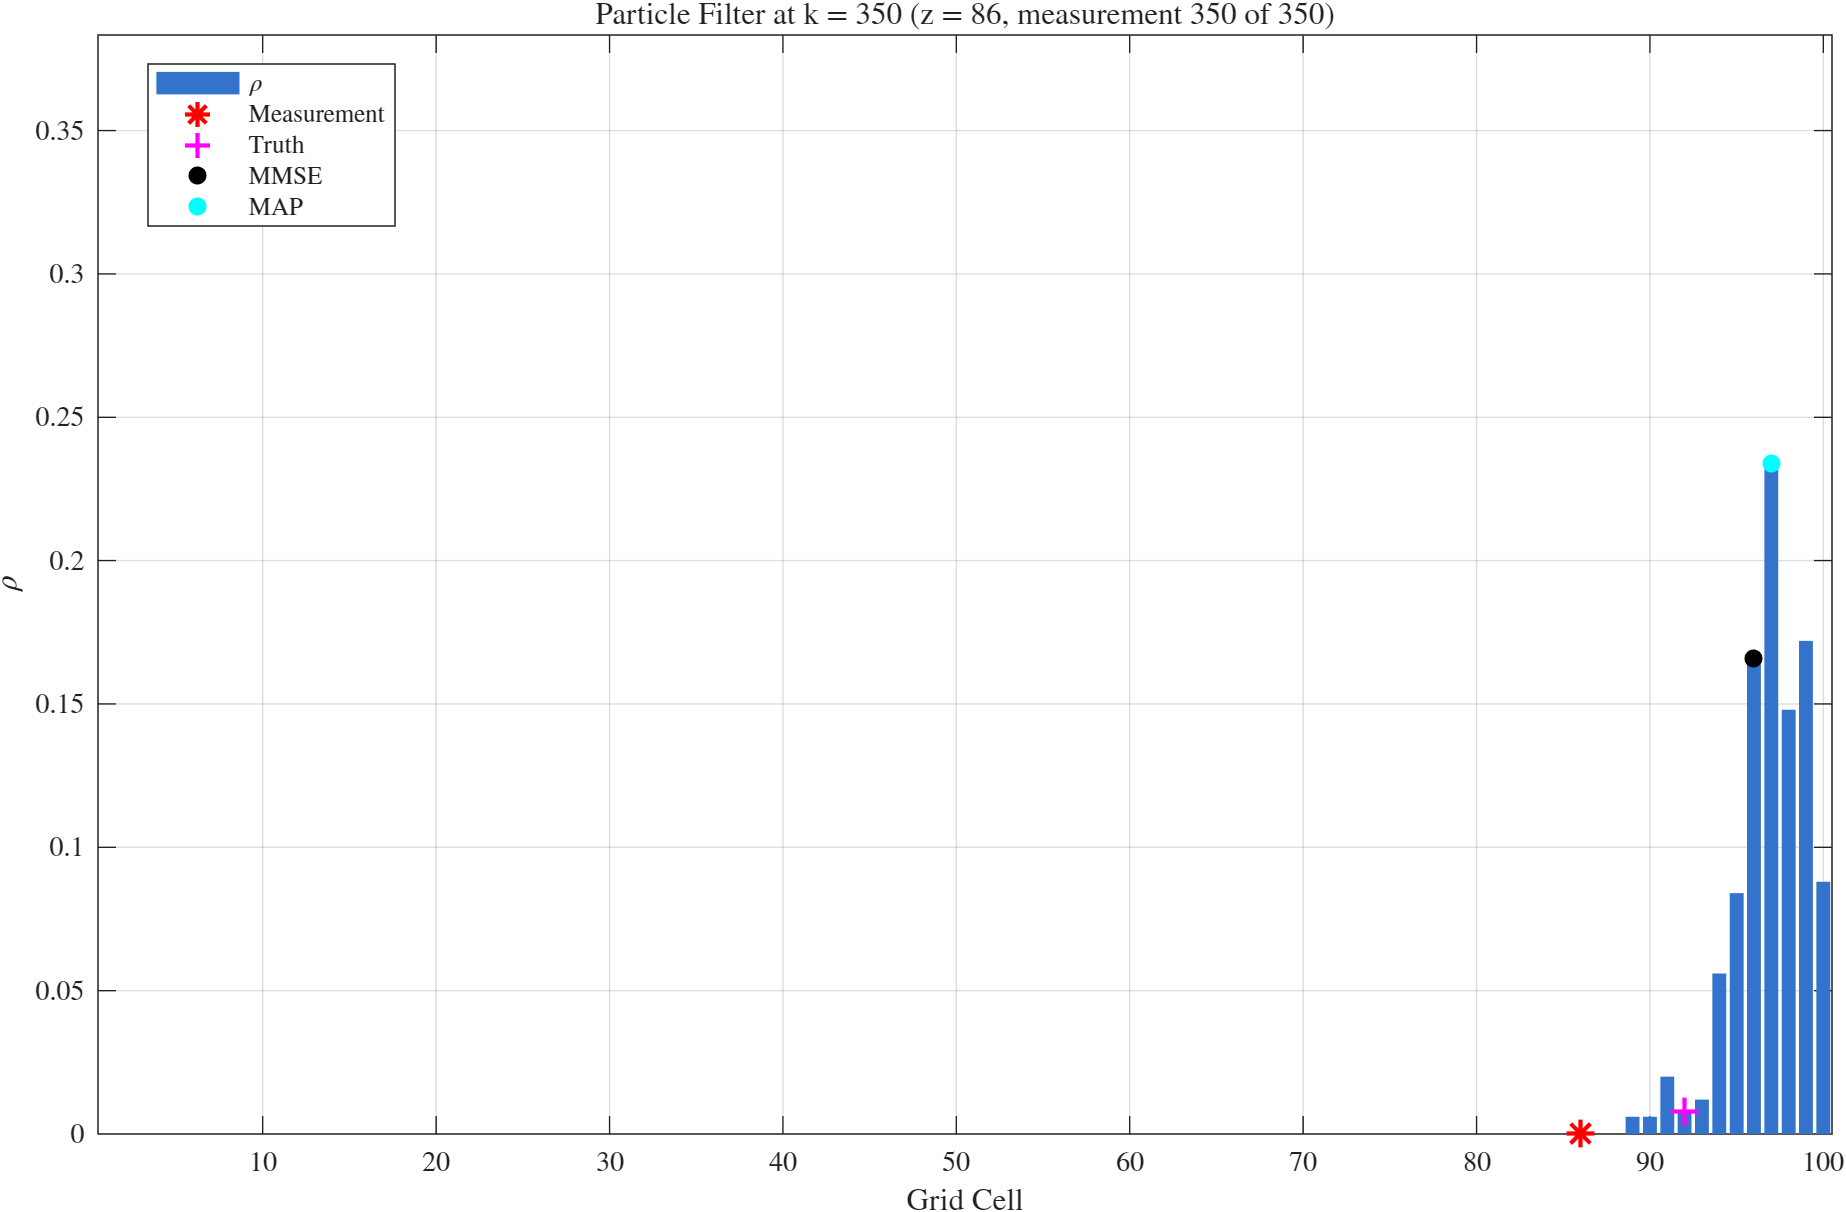
\includegraphics[width=\linewidth]{pf_filter_frame_350.png}
	                    \caption{$k=350$}
	                    \label{fig:pf350}
	                \end{subfigure}

	                \caption{PF posterior snapshots at selected timesteps.}
	                \label{fig:pf_filter_snapshots}
		            \end{figure}
	            \begin{table}[H]
	                \centering
	                \caption{PF MMSE and MAP estimates at selected timesteps}
	                \label{tab:PF_mmse_map}
	                \begin{tabular}{cccc}
	                    \toprule
	                    Timestep $k$ & MMSE Cell Index & MAP Cell Index & Ground Truth\\
	                    \midrule
	                    7   & 5 & 4 & 7\\
	                    50  & 32 & 31 & 30\\
	                    180 & 66 & 67 & 66\\
	                    300 & 81 & 82 & 82\\
	                    350 & 96 & 98 & 93\\
	                    \bottomrule
	                \end{tabular}
                \end{table}
                \begin{figure}[H]
                    \begin{subfigure}[t]{0.48\textwidth}
                        \centering
                        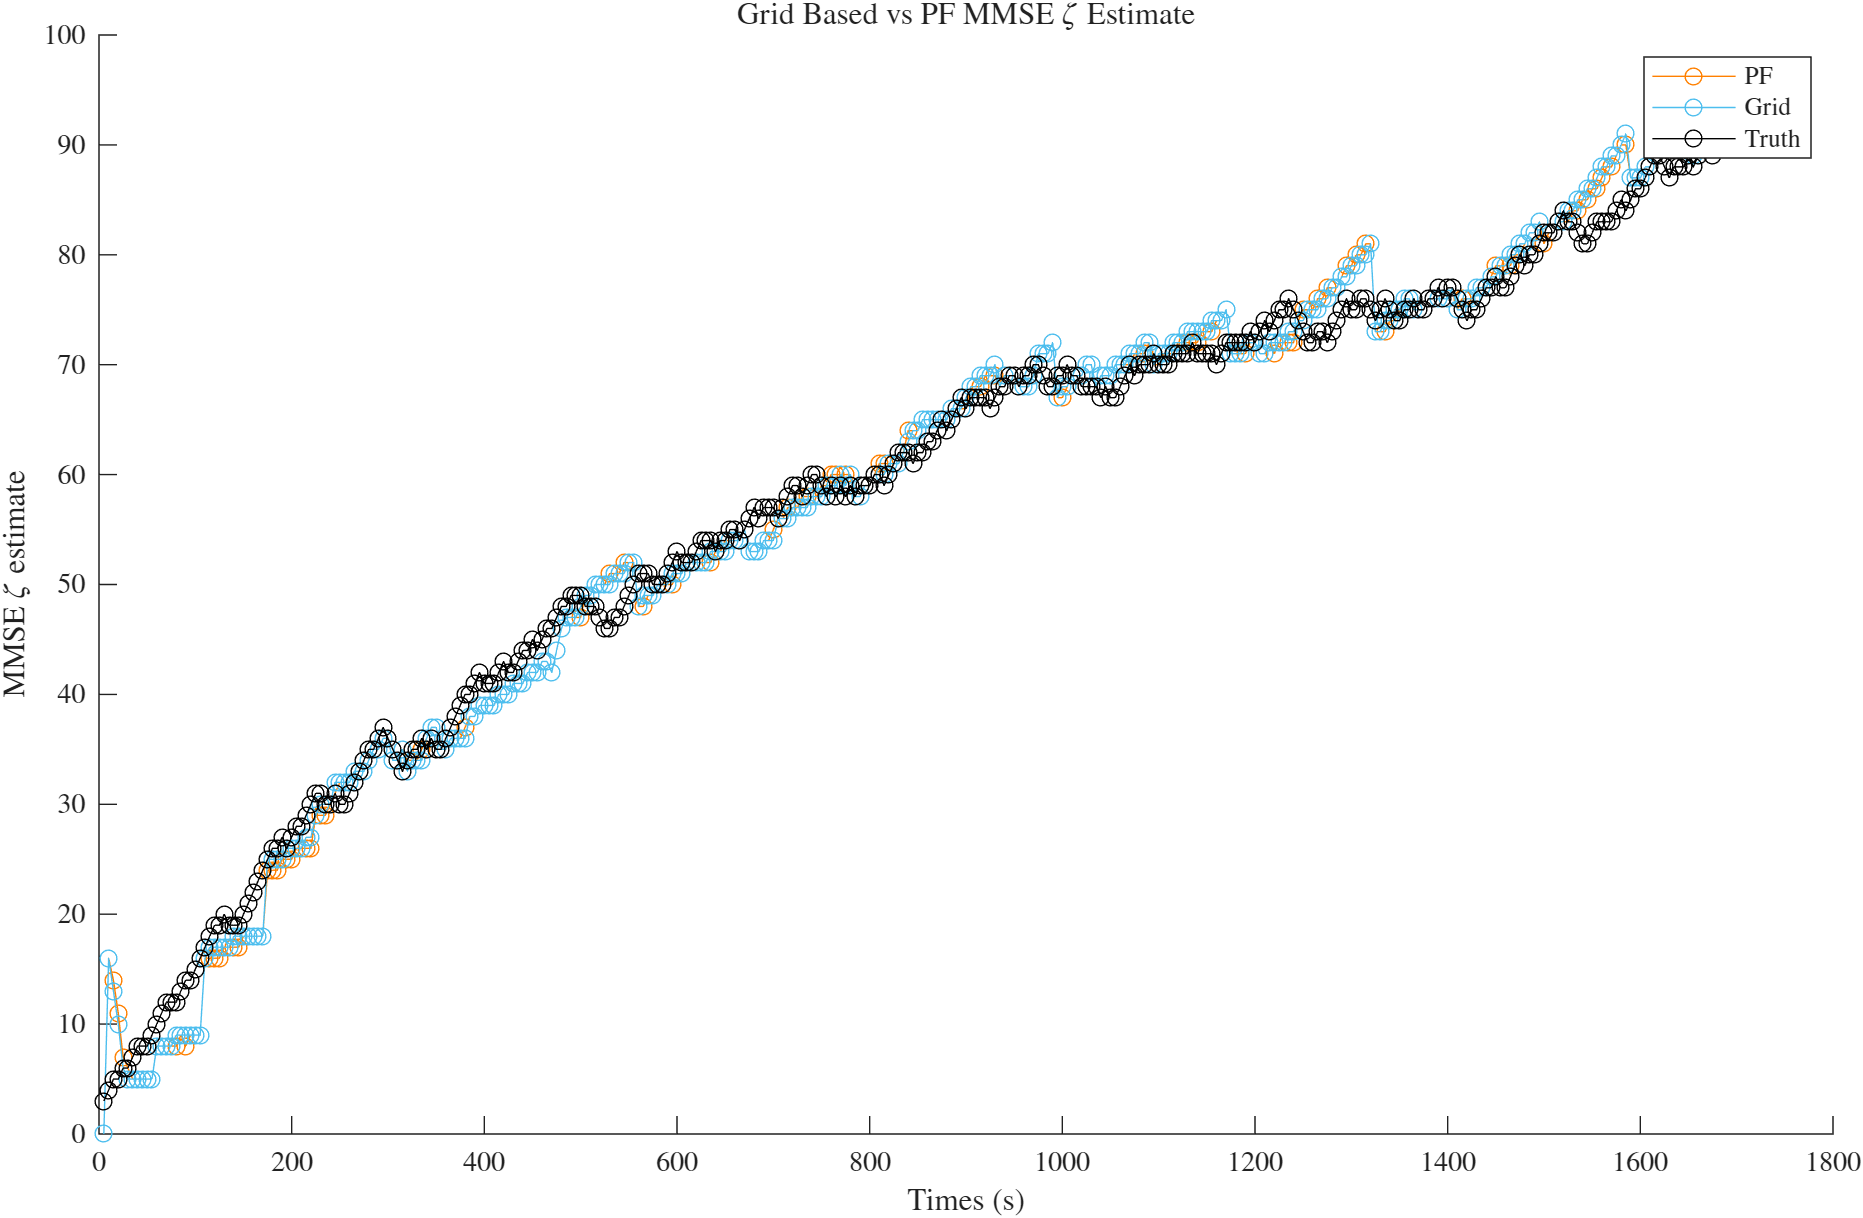
\includegraphics[width=\linewidth]{mmse_estimate_comparison.png}
                        \caption{MMSE $\zeta$ estimates for both grid and PF}
                        \label{fig:MMSEtot}
                    \end{subfigure}
                    \hfill
                    \begin{subfigure}[t]{0.48\textwidth}
                        \centering
                        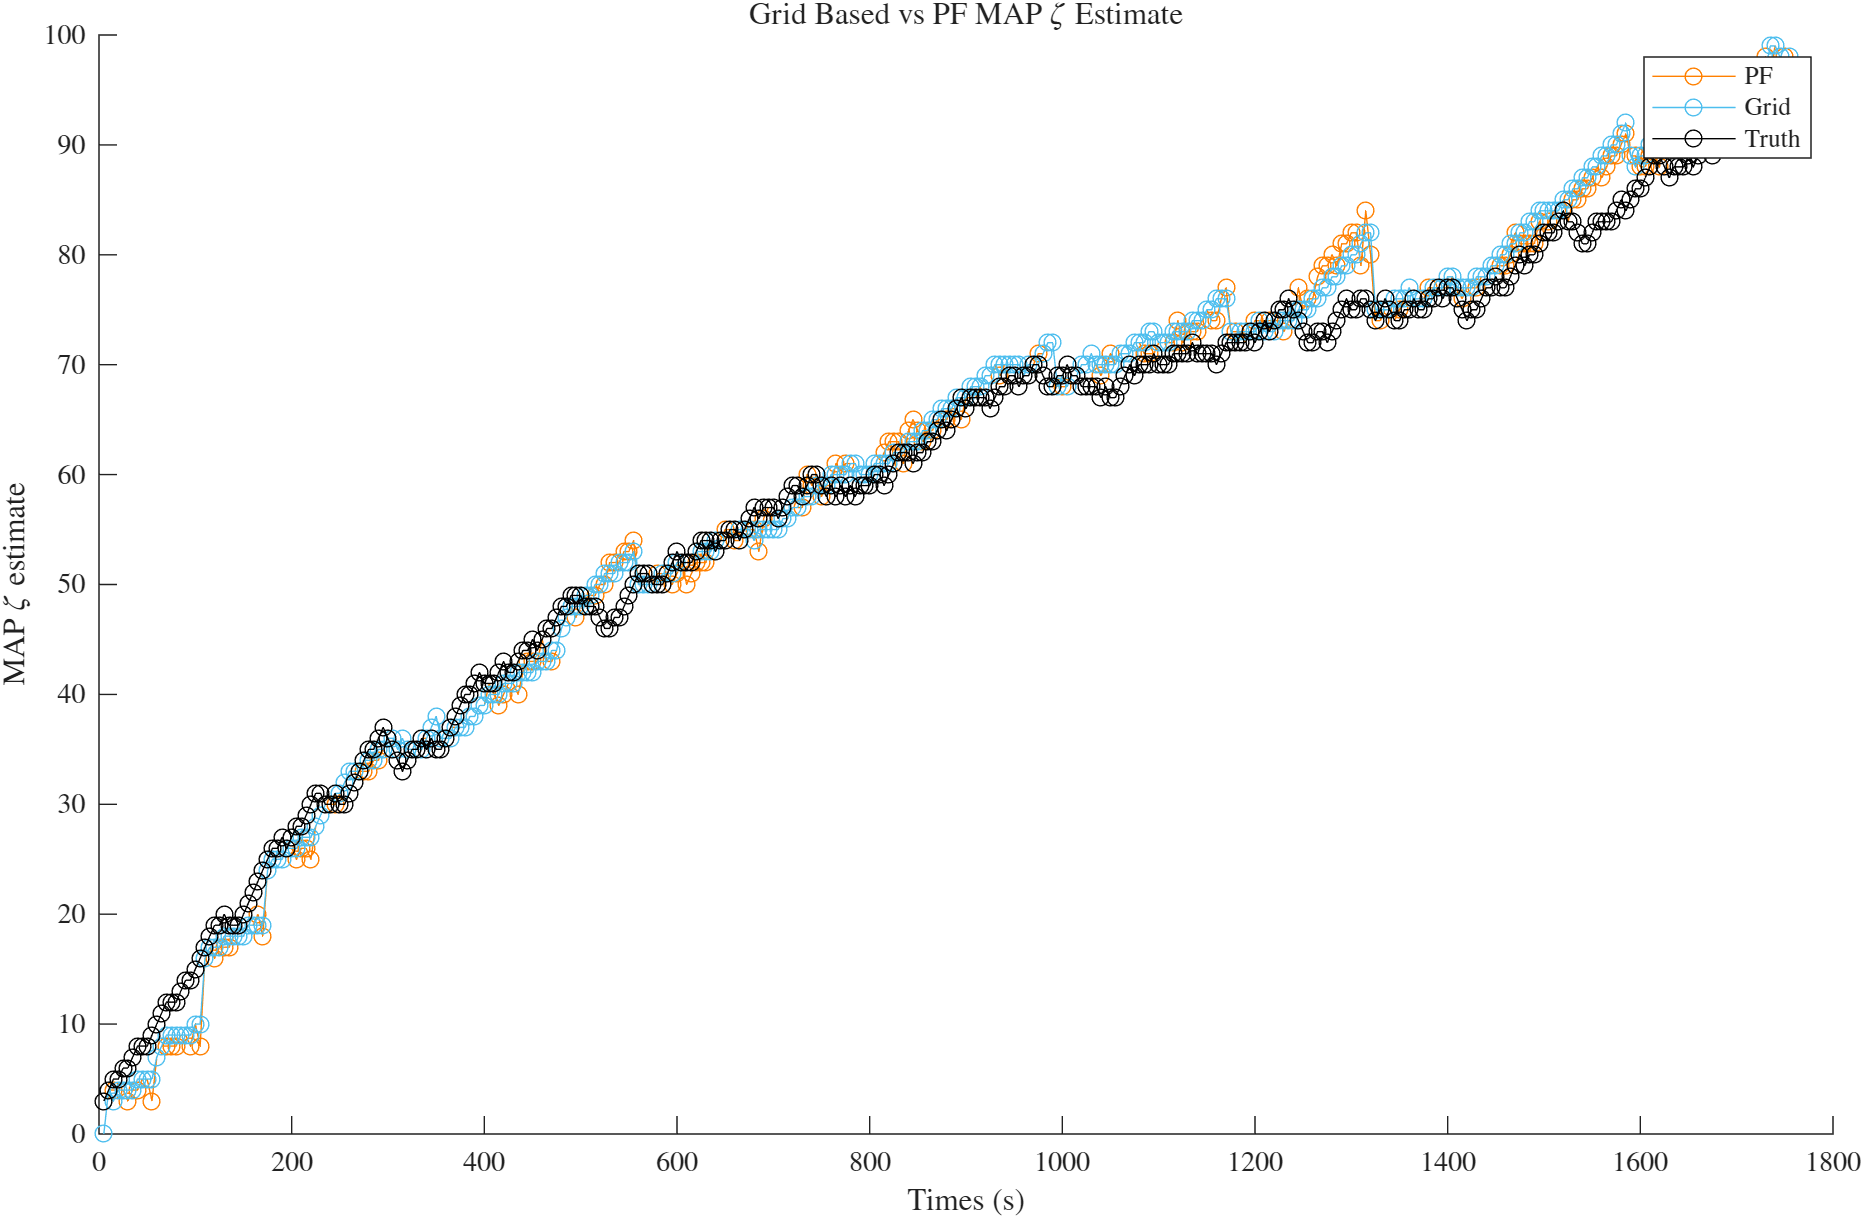
\includegraphics[width=\linewidth]{map_estimate_comparison.png}
                        \caption{MAP $\zeta$ estimates for both grid and PF}
                        \label{fig:MAPtot}
                    \end{subfigure}
                \caption{Grid and PF $\zeta$ estimates}
                \label{fig:tot}
                \end{figure}
        \end{enumerate}

\subsection{Code For Problem 2}

\begin{lstlisting}[style = matlab]

clear; clc; close all
load("asen6044hw3_problem2.mat")

set(groot, 'defaultTextInterpreter', 'latex')
set(groot, 'defaultAxesTickLabelInterpreter', 'latex')
set(groot, 'defaultLegendInterpreter', 'latex')

%% Declare Constants

rng(400)
r = 25;
L = 1000;
dx = 10;
dt = 5;
Nx = 100;

%% Part a) Get T and rho_inf

T = getT(Nx);

[V,D] = eig(T);

idx = find(abs(diag(D) - 1) < 1e-10); 
rhoinf = V(:, idx);
% corresponding eigenvector
rhoinf(rhoinf < 0) = 0; 
rhoinf= rhoinf./sum(rhoinf); % Normalize

%% Part b

rho0 = zeros(Nx,1);
rho0(3) = 1/3;
rho0(19) = 1/3;
rho0(35) = 1/3;

% prop_rho_kSteps(rho0,T,10, true);
% prop_rho_kSteps(rho0,T,50, true);
% prop_rho_kSteps(rho0,T,180, true);
% prop_rho_kSteps(rho0,T,300, true);
% prop_rho_kSteps(rho0,T,600, true);
% prop_rho_kSteps(rhoinf,T,0, true);

%% Part c


saveGridGif = true;
gifFile = "grid_filter.gif";
saveFrames = [7 50 180 300 350];
gridGif(zMeasHist,rho0,T,r,zetaHist, 'SaveGif', saveGridGif, 'GifFile', gifFile, 'SaveFrames', saveFrames);

%% Part d

% Initialize PF
particles = cell(1,length(zMeasHist));

Ns = 500;

InitCells = [3 19 35];

random_indices = randi([1, length(InitCells)], Ns, 1);

particles{1}.x = InitCells(random_indices);
particles{1}.w = 1/Ns * ones(1,Ns);
particles{1}.MMSE = 0;
particles{1}.MAP = 0;
particles{1}.Nx = Nx;

for i = 2:length(zMeasHist)
    particles{i} = PF(particles{i-1},T,zMeasHist(i),Ns);
end


PFgif(zMeasHist,particles{1},T,zetaHist,rho0,'SaveGif',true,'GifFile',"pf_filter.gif",'SaveFrames',saveFrames);

%%% MMSE and MAP comparison
Nm = length(zMeasHist);
rho_prior = rho0;
MMSE_Grid = zeros(1,Nm);
MAP_Grid = zeros(1,Nm);
MMSE_PF = zeros(1,Nm);
MAP_PF = zeros(1,Nm);
Like = meas_like(r,Nx);
Nm = length(zMeasHist);
for k = 2:Nm
    rho_minus = T * rho_prior;
    rho_plot = Like(zMeasHist(k), :)' .* rho_minus;
    rho_plot = rho_plot ./ sum(rho_plot);
    MMSE_Grid(k) = getMMSE(rho_plot);
    MAP_Grid(k) = getMAP(rho_plot);
    MMSE_PF(k) = particles{k}.MMSE;
    MAP_PF(k) = particles{k}.MAP;
    rho_prior = rho_plot;
end

figure; hold on
tvec = dt:dt:dt*Nm;
plot(tvec,MMSE_PF,"-o","Color",[1, 0.5, 0])
plot(tvec,MMSE_Grid,"-o", "Color",[0.3010, 0.7450, 0.9330])
plot(tvec,zetaHist,"k-o")
xlabel("Times (s)")
ylabel("MMSE $\zeta$ estimate")
title("Grid Based vs PF MMSE $\zeta$ Estimate")
legend("PF","Grid","Truth")
exportgraphics(gcf, "mmse_estimate_comparison.png", "Resolution", 200);

figure; hold on
tvec = dt:dt:dt*Nm;
plot(tvec,MMSE_PF-zetaHist,"-o","Color",[1, 0.5, 0])
plot(tvec,MMSE_Grid-zetaHist,"-o", "Color",[0.3010, 0.7450, 0.9330])
xlabel("Times (s)")
ylabel("MMSE $\zeta$ estimate error")
title("Grid Based vs PF MMSE $\zeta$ Estimate Error")
legend("PF","Grid")
exportgraphics(gcf, "mmse_error_comparison.png", "Resolution", 200);

figure; hold on
tvec = dt:dt:dt*Nm;
plot(tvec,MAP_PF,"-o","Color",[1, 0.5, 0])
plot(tvec,MAP_Grid,"-o", "Color",[0.3010, 0.7450, 0.9330])
plot(tvec,zetaHist,"k-o")
xlabel("Times (s)")
ylabel("MAP $\zeta$ estimate")
title("Grid Based vs PF MAP $\zeta$ Estimate")
legend("PF","Grid","Truth")
exportgraphics(gcf, "map_estimate_comparison.png", "Resolution", 200);

figure; hold on
tvec = dt:dt:dt*Nm;
plot(tvec,MAP_PF-zetaHist,"-o","Color",[1, 0.5, 0])
plot(tvec,MAP_Grid-zetaHist,"-o", "Color",[0.3010, 0.7450, 0.9330])
xlabel("Times (s)")
ylabel("MAP $\zeta$ estimate error")
title("Grid Based vs PF MAP $\zeta$ Estimate Error")
legend("PF","Grid")
exportgraphics(gcf, "map_error_comparison.png", "Resolution", 200);

%% Helper Functions

function [particles] = PF(particles,T,z,Ns)

r = 25;
Nx = size(T,1);

Like = meas_like(r,Nx);

x = particles.x;
w = particles.w;

xp = zeros(1,Ns);
wp = zeros(1,Ns);

for i = 1:Ns
    % Bootstrap PF proposal: sample x_k^i ~ p(x_k | x_{k-1}^i)
    xp(i) = sampleState(T(:,x(i)));

    % SIS weight update: w_k^i proportional to w_{k-1}^i * p(z_k | x_k^i)

    wp(i) = Like(z,xp(i))/Ns;
end

wp = wp./sum(wp);

particles.MMSE = floor(sum(xp .* wp));
particles.MAP = getParticleMAP(xp,wp,Nx);

% RESAMPLE
for i = 1:Ns
    p_idx = sampleState(wp);
    particles.x(i) = xp(p_idx);
end

particles.w = 1/Ns * ones(1,Ns);
particles.Nx = Nx;

end

function [] = plotPF(p, Ns, k, rho0,varargin)

    z = NaN;
    zeta = NaN;
    fig = [];
    
    if mod(numel(varargin),2) ~= 0
        error('Optional inputs must be provided as name/value pairs.');
    end
    
    for i = 1:2:numel(varargin)
        name = lower(string(varargin{i}));
        value = varargin{i+1};
    
        switch name
            case "measurement"
                z = value;
            case "truth"
                zeta = value;
            case "figure"
                fig = value;
            otherwise
                error("Unknown option '%s'.", varargin{i});
        end
    end
    
    if isempty(fig)
        figure;
    else
        figure(fig);
    end
    
    clf;
    hold on;
    grid on;
    box on;
    
    if isfield(p, 'Nx')
        Nx = p.Nx;
    else
        Nx = max(p.x(:));
    end

    rho = particlesToRho(p, Nx);
    MMSE = getMMSE(rho);
    MAP = getMAP(rho);

    bar(1:Nx, rho, 'FaceColor', [0.2 0.45 0.8], 'EdgeColor', 'none', ...
        'DisplayName', '$\rho$');
    
    
    if ~isnan(z)
        plot(z, rho(z), 'r*', 'MarkerSize', 10, 'LineWidth', 1.5, ...
            'DisplayName', 'Measurement');
    end
    
    if ~isnan(zeta)
        plot(zeta, rho(zeta), 'm+', 'MarkerSize', 10, 'LineWidth', 1.5, ...
            'DisplayName', 'Truth');
    end
    
    plot(MMSE, rho(MMSE), 'ko', 'MarkerFaceColor', 'k', 'MarkerSize', 6, ...
        'DisplayName', 'MMSE');
    plot(MAP, rho(MAP), 'co', 'MarkerFaceColor', 'c', 'MarkerSize', 6, ...
        'DisplayName', 'MAP');
    
    xlim([0.5, Nx + 0.5])
    ylim([0, max([rho0(:); rho(:)]) * 1.15 + eps]);    
    xlabel('Grid Cell')
    ylabel('$\rho$')
    title("PF estimated distribution at timestep k = " + num2str(k))
    legend('Location', 'best')
    
    hold off;

end

function [] = PFgif(z,particles0,T,zeta,rho0,varargin)
Ns = numel(particles0.x);

saveGif = false;
gifFile = "pf_filter.gif";
delayTime = 0.35;
saveFrames = [];

if mod(numel(varargin),2) ~= 0
    error('Optional inputs must be provided as name/value pairs.');
end

for i = 1:2:numel(varargin)
    name = lower(string(varargin{i}));
    value = varargin{i+1};

    switch name
        case "savegif"
            saveGif = logical(value);
        case "giffile"
            gifFile = string(value);
        case "delaytime"
            delayTime = value;
        case "saveframes"
            saveFrames = value(:)';
        otherwise
            error("Unknown option '%s'.", varargin{i});
    end
end

particles = particles0;
numMeas = numel(z);
measIdx = find(~isnan(z(:)));

fig = figure;
for k = 1:numMeas
    if k > 1
        particles = PF(particles,T,z(k),Ns);
    end

    plotPF(particles, Ns, k-1, rho0,...
        'Measurement', z(k), ...
        'Truth', zeta(k), ...
        'Figure', fig);

    if k == 1
        title('Initial Particle Prior at k = 0');
    elseif isnan(z(k))
        title(sprintf('Particle Prior at k = %d (no measurement)', k-1));
    else
        title(sprintf('Particle Filter at k = %d (z = %d, measurement %d of %d)', ...
            k-1, z(k), find(measIdx == k, 1), numel(measIdx)));
    end

    drawnow;

    if saveGif
        frame = getframe(fig);
        [imind, cm] = rgb2ind(frame2im(frame), 256);
        if k == 1
            imwrite(imind, cm, char(gifFile), 'gif', 'LoopCount', inf, ...
                'DelayTime', delayTime);
        else
            imwrite(imind, cm, char(gifFile), 'gif', 'WriteMode', 'append', ...
                'DelayTime', delayTime);
        end
    end

    if any(saveFrames == k-1)
        saveGifFrame(fig, gifFile, k-1);
    end
end
end

function [idx] = sampleState(p)
    
    c = cumsum(p);
    u = rand;
    idx = find(u <= c, 1, 'first');

end

function [MAP] = getParticleMAP(x,w,Nx)
    mass = accumarray(x(:), w(:), [Nx 1]);
    MAP = find(mass == max(mass), 1, 'first');
end

function [rho] = particlesToRho(p, Nx)
x = p.x(:);
w = p.w(:);
rho = accumarray(x, w, [Nx 1]); % Sum probability mass at each grid cell.
rho = rho ./ sum(rho);
end

function [] = saveGifFrame(fig, gifFile, k)
    [folder, name, ~] = fileparts(char(gifFile));
    pngFile = fullfile(folder, sprintf('%s_frame_%03d.png', name, k));
    exportgraphics(fig, pngFile, 'Resolution', 200);
end

function [T] = getT(Nx)

T = zeros(Nx);
for i = 1:Nx
    for j = 1:Nx
        if i == j && i > 1 && i <= Nx-1
            T(i,j) = 0.3;
        elseif i == j+1 && i > 2 && j >= 2
            T(i,j) = 0.5;
        elseif i == j-1 && i <= Nx-2 && j <= Nx-1
            T(i,j) = 0.2;
        elseif i == 1 && j == 1
            T(i,j) = 0.1;
        elseif i == Nx && j == Nx
            T(i,j) = 0.1;
        elseif i == 2 && j == 1
            T(i,j) = 0.9;
        elseif i == Nx-1 && j ==Nx
            T(i,j) = 0.9;
        end
    end
end
end

%% Plot rho dist as bar plot
function [] = plotRho(rho,k,z)

if nargin < 3
    z = NaN;
end

figure;
hold on;
grid on;

bar(rho, 'DisplayName', '$\rho$')
if ~isnan(z)
    plot(z,rho(z)+0.03, 'r*', 'MarkerSize', 12, 'LineWidth', 2, ...
        'DisplayName', 'Measurement')
end
title("$\rho^-$ propogated " + num2str(k) + " steps.")
legend('Location', 'best')
exportgraphics(gcf, sprintf('rho_propagated_%03d.png', k), 'Resolution', 200);

end

%% Propogate + Plot
function [rho_minus] = prop_rho_kSteps(rho0,T,k, PLOT)

rho_minus = T^k * rho0;

if PLOT
    plotRho(rho_minus,k)
end

end

%% Measurment Likelihood Matrix
function [L] = meas_like(r,Nx)
L = zeros(Nx);
for j = 1:Nx

    a = max([1, j-r]);
    b = min([Nx, j+r]);

    U = 1/(b-a+1);

    for i = 1:Nx
        if i >= a && i <= b
            L(i,j) = U;
        end
    end
end

end

%% Grid Bayes Filter
function [rho_plus] = prop_rho_kSteps_wMeas(z,rho0,T,k, r,Nx,PLOT)
Like = meas_like(r,Nx); % Const for each timestep
rho_prior = rho0;
for j = 1:k-1
    rho_minus = T*rho_prior;
    rho_plus = Like(z(j+1),:)'.*rho_minus;
    rho_plus = rho_plus./sum(rho_plus);
    rho_prior = rho_plus;
end
if PLOT
    plotRho(rho_plus,k,z(k))
end
end

%% Full Grid Bayes Filter Gif
function [] = gridGif(z,rho0,T,r,zeta,varargin)
Nx = size(T,1);

saveGif = false;
gifFile = "grid_filter.gif";
delayTime = 0.35;
saveFrames = [];

if mod(numel(varargin),2) ~= 0
    error('Optional inputs must be provided as name/value pairs.');
end

for i = 1:2:numel(varargin)
    name = lower(string(varargin{i}));
    value = varargin{i+1};

    switch name
        case "savegif"
            saveGif = logical(value);
        case "giffile"
            gifFile = string(value);
        case "delaytime"
            delayTime = value;
        case "saveframes"
            saveFrames = value(:)';
        otherwise
            error("Unknown option '%s'.", varargin{i});
    end
end

Like = meas_like(r,Nx);
rho_prior = rho0(:);
numMeas = numel(z);
measIdx = find(~isnan(z(:)));

fig = figure;
    for k = 1:numMeas
        clf(fig);

    if k == 1 || isnan(z(k))
        rho_plot = rho_prior;
        bar(1:Nx, rho_plot, 'FaceColor', [0.2 0.45 0.8], 'EdgeColor', 'none', ...
            'DisplayName', '$\rho$');
        if k == 1
            title('Initial Prior at k = 0');
        else
            title(sprintf('Prior at k = %d (no measurement)', k-1));
        end
        legend('Location', 'best');
    else
        rho_minus = T * rho_prior;
        rho_plot = Like(z(k), :)' .* rho_minus;
        rho_plot = rho_plot ./ sum(rho_plot);
        MMSE = getMMSE(rho_plot);
        MAP = getMAP(rho_plot);
        bar(1:Nx, rho_plot, 'FaceColor', [0.2 0.45 0.8], 'EdgeColor', 'none', ...
            'DisplayName', '$\rho$');
        hold on;
        plot(z(k), rho_plot(z(k)), 'r*', 'MarkerSize', 10, 'LineWidth', 1.5, ...
            'DisplayName', 'Measurement');
        plot(MMSE, rho_plot(MMSE), 'ko', 'MarkerSize', 10, 'LineWidth', 1.5, ...
            'DisplayName', 'MMSE');
        plot(MAP, rho_plot(MAP), 'co', 'MarkerSize', 10, 'LineWidth', 1.5, ...
            'DisplayName', 'MAP');
        plot(zeta(k),rho_plot(zeta(k)), 'm+', 'MarkerSize', 10, 'LineWidth', 1.5, ...
            'DisplayName', 'Truth');
        hold off;
        legend('Location', 'best');
        title(sprintf('Grid Filter Posterior at k = %d (z = %d, measurement %d of %d)', ...
            k-1, z(k), find(measIdx == k, 1), numel(measIdx)));
        rho_prior = rho_plot;
    end

    grid on;
    xlim([0.5, Nx + 0.5]);
    ylim([0, max([rho0(:); rho_plot(:)]) * 1.15 + eps]);
    xlabel('Grid Cell');
    ylabel('$\rho$');

    drawnow;

    if saveGif
        frame = getframe(fig);
        [imind, cm] = rgb2ind(frame2im(frame), 256);
        if k == 1
            imwrite(imind, cm, char(gifFile), 'gif', 'LoopCount', inf, ...
                'DelayTime', delayTime);
        else
            imwrite(imind, cm, char(gifFile), 'gif', 'WriteMode', 'append', ...
                'DelayTime', delayTime);
        end
    end

    if any(saveFrames == k-1)
        saveGifFrame(fig, gifFile, k-1);
    end
end
end

function [MMSE] = getMMSE(rho)

MMSE = 0;
for j = 1:length(rho)
    MMSE = MMSE + rho(j)*j;
end
MMSE = floor(MMSE);
end

function [MAP] = getMAP(rho)
MAP = find(rho == max(rho));
end

\end{lstlisting}




% =====================================================

\end{document}
